\setcounter{ex}{0}
\setcounter{dang}{0}
\Opensolutionfile{ans}[ans/CD14/Muc10]
\begin{ex}%[2H1G3-4]
	Cho hình hộp $ABCD.A'B'C'D'$ có chiều cao bằng $8$ và diện tích đáy bằng $9$. Gọi $M$, $N$, $P$ và $Q$ lần lượt là tâm của các mặt bên $ABB'A'$, $BCC'B'$, $CDD'C'$ và $DAA'D'$ . Thể tích của khối đa diện lồi có các đỉnh là các điểm $A$, $B$, $C$, $D$, $M$, $N$, $P$ và $Q$ bằng
	\choice
	{$27$}
	{\True $30$}
	{$18$}
	{$36$}
	\loigiai{
		\immini{Gọi $E$, $F$, $G$, $H$ lần lượt là trung điểm của $AA'$, $BB'$, $CC'$, $DD'$.\\
			Khi đó $V_{ABCD.EFGH}=\dfrac12V_{ABCD.A'B'C'D'}=\dfrac12\cdot9\cdot8=36$\\
			Gọi $V$ là thể tích khối đa diện lồi cần tính, khi đó\\ $V=V_{ABCD.EFGH}-V_{E.AMQ}-V_{F.BMN}-V_{G.CNP}-V_{H.DPQ}$.\\
			Trong đó $V_{E.AMQ}=V_{F.BMN}=V_{G.CNP}=V_{H.DPQ}$\\ $=\dfrac{EQ}{EH}\cdot\dfrac{EM}{EF}\cdot V_{E.AHF}=\dfrac14\cdot\dfrac16\cdot V_{ABCD.EFGH}=\dfrac{36}{24}=\dfrac32$\\
			$\Rightarrow V=36-4\cdot\dfrac32=30$.}
		{
			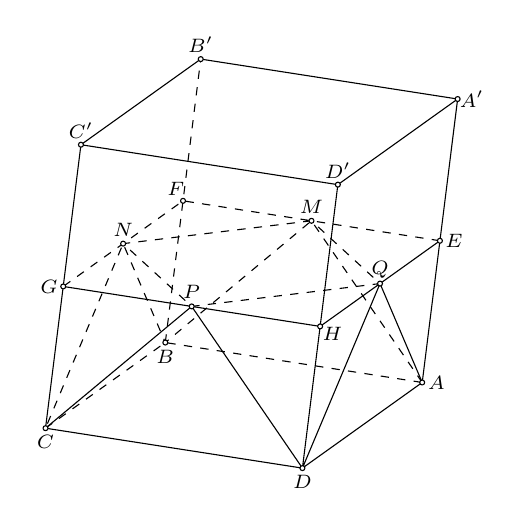
\begin{tikzpicture}[line join=round,font=\scriptsize,scale=.9]
				\def\a{4}
				\pgfmathsetmacro{\am}{\a *sqrt(2)}
				\pgfmathsetmacro{\bm}{\am/3}
				\pgfmathsetmacro{\g}{20}
				\pgfmathsetmacro{\xa}{\am *cos(\g)/2}
				\pgfmathsetmacro{\ya}{\bm *sin(\g)/2}
				\pgfmathsetmacro{\xb}{\am *cos(\g+90)/2}
				\pgfmathsetmacro{\yb}{\bm *sin(\g+90)/2}
				\path(0,0)coordinate(O)
				(.5,\a)coordinate(O')
				(\xa,\ya)coordinate(A)
				(\xb,\yb)coordinate(B)
				(-\xa,-\ya)coordinate(C)
				(-\xb,-\yb)coordinate(D)
				(A)+(O')coordinate(A')
				(B)+(O')coordinate(B')
				(C)+(O')coordinate(C')
				(D)+(O')coordinate(D')
				(barycentric cs:A=1,B'=1)coordinate(M)
				(barycentric cs:B=1,C'=1)coordinate(N)
				(barycentric cs:C=1,D'=1)coordinate(P)
				(barycentric cs:D=1,A'=1)coordinate(Q)
				(barycentric cs:A=1,A'=1)coordinate(E)
				(barycentric cs:B=1,B'=1)coordinate(F)
				(barycentric cs:C=1,C'=1)coordinate(G)
				(barycentric cs:D=1,D'=1)coordinate(H);
				\draw[dashed] (C)--(B)--(A)(B)--(B');
				\draw[dashed] (M)--(N)--(P)--(Q)--cycle (E)--(F)--(G)
				(A)--(M)--(B)--(N)--(C);
				\draw (A')--(A)--(D)--(D')(C')--(C)--(D) (A')--(B')--(C')--(D')--cycle
				(G)--(H)--(E)(C)--(P)--(D)--(Q)--(A);
				\foreach \p/\q in{A/0,B/-90,C/-90,D/-90,A'/0,B'/90,C'/90,D'/90,M/90,N/90,P/90,Q/90,E/0,F/120,G/180,H/-30}\draw[fill=white](\p)circle(1pt)+(\q:.2)node{$\p$};
		\end{tikzpicture}}
	}
\end{ex}

\begin{ex}%[2H1G3-4]
	Cho hình chóp đều $ S.ABCD$ có cạnh đáy bằng $ a$, cạnh bên bằng $ 2a$ và $ O$ là tâm của đáy. Gọi $ M$,$ N$, $ P$, $ Q$ lần lượt là các điểm đối xứng với $ O$ qua trọng tâm của các tam giác $ SAB$, $ SBC$, $ SCD$, $ SDA$ và $ S'$ là điểm đối xứng với $ S$ qua $O$. Thể tích của khối chóp $ S'.MNPQ$ bằng
	\choice
	{\True $\dfrac{20\sqrt{14}{a^3}}{81}$}
	{$\dfrac{40\sqrt{14}{a^3}}{81}$}
	{$\dfrac{10\sqrt{14}{a^3}}{81}$}
	{$\dfrac{2\sqrt{14}{a^3}}{9}$}
	\loigiai{
		\begin{center}
			\begin{tikzpicture}[>=stealth, scale=1,samples=100,smooth]
				% \clip (-3.5,-2.5) rectangle (4.5,4.5);
				\def\h{7}
				\coordinate (O) at (0,0);
				\coordinate (S) at (0,\h);
				\coordinate (A) at (-2,1);
				\coordinate (B) at (-6,-1.5);
				\coordinate (C) at ($(A)!2!(O)$);
				\coordinate (D) at ($(B)!2!(O)$);
				\coordinate (E) at ($(A)!0.5!(B)$);
				\coordinate (F) at ($(B)!0.5!(C)$);
				\coordinate (G) at ($(C)!0.5!(D)$);
				\coordinate (H) at ($(A)!0.5!(D)$);
				\tkzCentroid(S,A,B) \tkzGetPoint{G1}
				\coordinate (M) at ($(O)!2!(G1)$);
				\tkzCentroid(S,B,C) \tkzGetPoint{G2}
				\coordinate (N) at ($(O)!2!(G2)$);
				\tkzCentroid(S,C,D) \tkzGetPoint{G3}
				\coordinate (P) at ($(O)!2!(G3)$);
				\tkzCentroid(S,A,D) \tkzGetPoint{G4}
				\coordinate (Q) at ($(O)!2!(G4)$);
				\coordinate (S') at ($(S)!2!(O)$);
				\path
				(intersection of S--B and M--G1) coordinate (L1)
				(intersection of S--B and M--Q) coordinate (L2)
				(intersection of S--D and M--Q) coordinate (L3)
				(intersection of S'--O and B--C) coordinate (L4);
				\draw (C)--(D)--(S)--(C)--(B)--(S)--(G) (M)--(N)--(P)--(Q) (L1)--(M)--(L2) (G2)--(N) (G3)--(P) (S)--(F) (L3)--(Q) (L4)--(S');
				\draw[dashed] (C)--(A)--(B)--(D)--(A)--(S)--(O) (S)--(E)--(F)--(G)--(H)--(E) (S)--(H) (G2)--(O)--(L1) (Q)--(O)--(G3)--(G2) (G1)--(G2) (G3)--(G4)--(G1) (L2)--(L3) (L4)--(O);
				\foreach \x/\g in {A/160,B/-90,C/-90,D/0,E/160,F/-90,G/-40,H/60,M/180,N/-90,P/0,Q/90/,O/-130,S/60,S'/0}
				\fill[black](\x) circle (1pt)
				($(\x)+(\g:3mm)$) node{\color{black}$\x$};
				\draw(G1)node[below left,yshift=0.1cm]{$G_1$} (G2) node[right,yshift=0.25cm]{$G_2$} (G3)node[right]{$G_3$} (G4)node[right]{$G_4$};
			\end{tikzpicture}
		\end{center}
		Gọi $G_1,G_2,G_3,G_4$ lần lượt là trọng tâm $\triangle SAB$, $\triangle SBC$, $\triangle SCD$, $\triangle SDA$ .\\
		$E$, $F$, $G$, $H$ lần lượt là trung điểm của các cạnh $AB$, $BC$, $CD$, $DA$ .\\
		Ta có $S_{MNPQ}=4S_{G_1G_2G_3G_4}=4.\dfrac{4}{9}{S_{EFGH}}=4.\dfrac{4}{9}\cdot\dfrac{1}{2}EG\cdot HF=\dfrac{8a^2}{9}$ .\\
		$\begin{array}{l}
			\mathrm{d}\left(S',\left(MNPQ\right)\right)=\mathrm{d}\left(S',\left(ABCD\right)\right)+\mathrm{d}\left(O,\left(MNPQ\right)\right)\\
			=\mathrm{d}\left(S,\left(ABCD\right)\right)+2\mathrm{d}\left(O,\left(G_1G_2G_3G_4\right)\right)\\
			=\mathrm{d}\left(S,\left(ABCD\right)\right)+\dfrac{2}{3}d\left(S,\left(ABCD\right)\right)\\
			=\dfrac{5}{3}\mathrm{d}\left(S,\left(ABCD\right)\right)=\dfrac{5a\sqrt{14}}{6}
		\end{array}$\\
		Vậy $V_{S'.MNPQ}=\dfrac{1}{3}\cdot\dfrac{5a\sqrt{14}}{6}\cdot\dfrac{8a^2}{9}=\dfrac{20a^3\sqrt{14}}{81}$.}
\end{ex}

\begin{ex}%[2H1G3-4]
	Cho hình chóp đều $S.ABCD$ có cạnh đáy bằng $a$, cạnh bên bằng $a\sqrt{3}$ và $O$ là tâm của đáy. Gọi $M$, $N$, $P$, $Q$ lần lượt là các điểm đối xứng với $O$ qua trọng tâm các tam giác $SAB$, $SBC$, $SCD$, $SDA$ và $S'$ là điểm đối xứng  với $S$ qua $O$. Thể tích của khối chóp $S'.MNPQ$ bằng
	\choice
	{$\dfrac{40\sqrt{10}a^{3}}{81}$}
	{$\dfrac{10\sqrt{10}a^{3}}{81}$}
	{\True $\dfrac{20\sqrt{10}a^{3}}{81}$}
	{$\dfrac{2\sqrt{10}a^{3}}{9}$}
	\loigiai{
		\begin{center}
			\begin{tikzpicture}[>=stealth, scale=.8,samples=100,smooth]
				% \clip (-3.5,-2.5) rectangle (4.5,4.5);
				\def\h{7}
				\coordinate (O) at (0,0);
				\coordinate (S) at (0,\h);
				\coordinate (A) at (-2,1);
				\coordinate (B) at (-6,-1.5);
				\coordinate (C) at ($(A)!2!(O)$);
				\coordinate (D) at ($(B)!2!(O)$);
				\coordinate (E) at ($(A)!0.5!(B)$);
				\coordinate (F) at ($(B)!0.5!(C)$);
				\coordinate (G) at ($(C)!0.5!(D)$);
				\coordinate (H) at ($(A)!0.5!(D)$);
				\tkzCentroid(S,A,B) \tkzGetPoint{G1}
				\coordinate (M) at ($(O)!2!(G1)$);
				\tkzCentroid(S,B,C) \tkzGetPoint{G2}
				\coordinate (N) at ($(O)!2!(G2)$);
				\tkzCentroid(S,C,D) \tkzGetPoint{G3}
				\coordinate (P) at ($(O)!2!(G3)$);
				\tkzCentroid(S,A,D) \tkzGetPoint{G4}
				\coordinate (Q) at ($(O)!2!(G4)$);
				\coordinate (S') at ($(S)!2!(O)$);
				\path
				(intersection of S--B and M--G1) coordinate (L1)
				(intersection of S--B and M--Q) coordinate (L2)
				(intersection of S--D and M--Q) coordinate (L3)
				(intersection of S'--O and B--C) coordinate (L4);
				\draw (C)--(D)--(S)--(C)--(B)--(S)--(C) (S)--(G) (M)--(N)--(P)--(Q) (L1)--(M)--(L2) (G2)--(N) (G3)--(P) (S)--(F) (L3)--(Q) (L4)--(S')--(P) (M)--(S')--(N);
				\draw[dashed] (C)--(A)--(B)--(D)--(A)--(S)--(O) (S)--(E)--(F)--(G)--(H)--(E) (S)--(H) (G2)--(O)--(L1) (Q)--(O)--(G3)--(G2) (G1)--(G2) (G3)--(G4)--(G1) (L2)--(L3) (L4)--(O) (Q)--(S');
				\foreach \x/\g in {A/160,B/-90,C/-90,D/0,O/-130,S/60,S'/0}
				\fill[black](\x) circle (1pt)
				($(\x)+(\g:3mm)$) node{\color{black}$\x$};
				\draw(G1)node[below left,yshift=0.1cm]{$G_1$} (G2) node[right,yshift=0.25cm]{$G_2$} (G3)node[right]{$G_3$} (G4)node[right]{$G_4$};
				\path
				(M)node[left]{$Q$}
				(Q)node[above]{$M$}
				(P)node[right]{$N$}
				(N)node[below]{$P$};
			\end{tikzpicture}
		\end{center}
		Ta gọi $G_1$, $G_2$, $G_3$, $G_4$ lần lượt là trọng tâm của tam giác $SAB$, $SBC$, $SCD$, $SDA$ thì
		\begin{eqnarray*}
			\mathrm{d}\left(S',\left(MNPQ\right)\right)&=& \dfrac{5}{2}\mathrm{d}\left(O,\left(MNPQ\right)\right)\\
			&\Rightarrow & {V_{S'.MNPQ}}=\dfrac{5}{2}{V_{O.MNPQ}}=\dfrac{5}{2}\cdot8V_{O.G_1G_2G_3G_4}\\
			&= & 10V_{S.G_1G_2G_3G_4}=10\cdot\dfrac{4}{27}{V_{S.ABCD}}\\
			& =&\dfrac{40}{27}\cdot\dfrac{1}{3}\cdot\dfrac{a\sqrt{10}}{2}\cdot a^2=\dfrac{20\sqrt{10}{a^3}}{81}.
		\end{eqnarray*}
	}
\end{ex}

\begin{ex}%[2H1G3-4]
	Cho hình chóp đều $S.ABCD$ có cạnh đáy bằng $a$, cạnh bên bằng $\sqrt 2a$ và $O$ là tâm của đáy. Gọi $M$, $N$, $P$, $Q$ lần lượt là các điểm đối xứng với $O$ qua trọng tâm của các tam giác $SAB$, $SBC$, $SCD$, $SDA$ và $S'$ là điểm đối xứng với $S$ qua $O$. Thể tích khối chóp $S'.MNPQ$ bằng.
	\choice
	{$\dfrac{2\sqrt 6a^3}{9}$}
	{$\dfrac{40\sqrt 6a^3}{81}$}
	{$\dfrac{10\sqrt 6a^3}{81}$}
	{\True $\dfrac{20\sqrt 6a^3}{81}$}
	\loigiai{
		\begin{center}
			\begin{center}
				\begin{tikzpicture}[>=stealth, scale=.8,samples=100,smooth]
					\def\h{7}
					\coordinate (O) at (0,0);
					\coordinate (S) at (0,\h);
					\coordinate (A) at (-2,1);
					\coordinate (B) at (-6,-1.5);
					\coordinate (C) at ($(A)!2!(O)$);
					\coordinate (D) at ($(B)!2!(O)$);
					\coordinate (E) at ($(A)!0.5!(B)$);
					\coordinate (F) at ($(B)!0.5!(C)$);
					\coordinate (G) at ($(C)!0.5!(D)$);
					\coordinate (H) at ($(A)!0.5!(D)$);
					\tkzCentroid(S,A,B) \tkzGetPoint{G1}
					\coordinate (M) at ($(O)!2!(G1)$);
					\tkzCentroid(S,B,C) \tkzGetPoint{G2}
					\coordinate (N) at ($(O)!2!(G2)$);
					\tkzCentroid(S,C,D) \tkzGetPoint{G3}
					\coordinate (P) at ($(O)!2!(G3)$);
					\tkzCentroid(S,A,D) \tkzGetPoint{G4}
					\coordinate (Q) at ($(O)!2!(G4)$);
					\coordinate (S') at ($(S)!2!(O)$);
					\coordinate (K) at ($(M)!0.5!(P)$);
					\path
					(intersection of S--B and M--G1) coordinate (L1)
					(intersection of S--B and M--Q) coordinate (L2)
					(intersection of S--D and M--Q) coordinate (L3)
					(intersection of S'--O and B--C) coordinate (L4)
					(intersection of S--B and M--P) coordinate (L5)
					(intersection of S--D and M--P) coordinate (L6)
					(intersection of S--D and N--Q) coordinate (L7)
					;
					\draw (C)--(D)--(S)--(C)--(B)--(S) (M)--(N)--(P)--(Q) (L1)--(M)--(L2) (G2)--(N) (G3)--(P) (L3)--(Q) (L4)--(S') (M)--(L5) (P)--(L6) (Q)--(L7);
					\draw[dashed] (C)--(A)--(B)--(D)--(A)--(S)--(O) (G2)--(O)--(L1) (Q)--(O)--(G3)--(G2) (G1)--(G2) (G3)--(G4)--(G1) (L2)--(L3) (L4)--(O) (L5)--(L6) (N)--(L7);
					\foreach \x/\g in {A/160,B/-90,C/-90,D/0,M/180,N/-90,P/0,Q/90/,O/-130,S/60,S'/0,K/120}
					\fill[black](\x) circle (1pt)
					($(\x)+(\g:3mm)$) node{\color{black}$\x$};
				\end{tikzpicture}
			\end{center}
		\end{center}
		Ta có $S'K=S'O+OK=SO+\dfrac{2}{3}SO=\dfrac{5a\sqrt 6}{6}\cdot $\\
		Ta có ${MNPQ}=4\cdot\dfrac{1}{2}\cdot\dfrac{4}{9}{S_{ABCD}}=\dfrac{8}{9}{a^2}.$\\
		Vậy $V_{S'.MNPQ}=\dfrac{20\sqrt 6a^3}{81}\cdot $}
\end{ex}

\begin{ex}%[2H1G3-4]
	Cho hình chóp đều $S.ABCD$ có tất cả các cạnh bằng $a$ và $O$ là tâm của đáy. Gọi $M$, $N$, $P$, $Q$ lần lượt là các điểm đối xứng với $O$ qua trọng tâm của các tam giác $SAB$, $SBC$, $SCD$, $SDA$ và $S'$ là điểm đối xứng với $S$ qua $O$. Thể tích khối chóp $S'.MNPQ$ bằng
	\choice
	{$\dfrac{2\sqrt 2a^3}{9}$}
	{\True $\dfrac{20\sqrt 2a^3}{81}$}
	{$\dfrac{40\sqrt 2a^3}{81}$}
	{$\dfrac{10\sqrt 2a^3}{81}$}
	\loigiai{
		\begin{center}
			\begin{tikzpicture}[>=stealth, scale=1,samples=100,smooth]
				\def\h{7}
				\coordinate (O) at (0,0);
				\coordinate (S) at (0,\h);
				\coordinate (A) at (-2,1);
				\coordinate (B) at (-6,-1.5);
				\coordinate (C) at ($(A)!2!(O)$);
				\coordinate (D) at ($(B)!2!(O)$);
				\coordinate (E) at ($(A)!0.5!(B)$);
				\coordinate (F) at ($(B)!0.5!(C)$);
				\coordinate (G) at ($(C)!0.5!(D)$);
				\coordinate (H) at ($(A)!0.5!(D)$);
				\tkzCentroid(S,A,B) \tkzGetPoint{G1}
				\coordinate (M) at ($(O)!2!(G1)$);
				\tkzCentroid(S,B,C) \tkzGetPoint{G2}
				\coordinate (N) at ($(O)!2!(G2)$);
				\tkzCentroid(S,C,D) \tkzGetPoint{G3}
				\coordinate (P) at ($(O)!2!(G3)$);
				\tkzCentroid(S,A,D) \tkzGetPoint{G4}
				\coordinate (Q) at ($(O)!2!(G4)$);
				\coordinate (S') at ($(S)!2!(O)$);
				\coordinate (I) at ($(M)!0.5!(P)$);
				\path
				(intersection of S--B and M--G1) coordinate (L1)
				(intersection of S--B and M--Q) coordinate (L2)
				(intersection of S--D and M--Q) coordinate (L3)
				(intersection of S'--O and B--C) coordinate (L4)
				(intersection of S--B and M--P) coordinate (L5)
				(intersection of S--D and M--P) coordinate (L6)
				(intersection of S--D and N--Q) coordinate (L7)
				;
				\draw (C)--(D)--(S)--(C)--(B)--(S) (M)--(N)--(P)--(Q) (L1)--(M)--(L2) (G2)--(N) (G3)--(P) (L3)--(Q) (L4)--(S') (M)--(L5) (L6)--(P) (L7)--(Q);
				\draw[dashed] (C)--(A)--(B)--(D)--(A)--(S)--(O)  (G2)--(O)--(L1) (Q)--(O)--(G3)--(G2) (G1)--(G2) (G3)--(G4)--(G1) (L2)--(L3) (L4)--(O) (L5)--(L6) (N)--(L7);
				\foreach \x/\g in {A/160,B/-90,C/-90,D/0,M/180,N/-90,P/0,Q/90/,O/-130,S/60,S'/0,I/120}
				\fill[black](\x) circle (1pt)
				($(\x)+(\g:3mm)$) node{\color{black}$\x$};
				\draw(G1)node[below left,yshift=0.1cm]{$G$} (G3)node[right]{$K$};
			\end{tikzpicture}
		\end{center}
		Ta có $SO=\dfrac{a\sqrt 2}{2}$\\
		Gọi $G,K$ lần lượt là trọng tâm của tam giác $SAB$ và tam giác $SCD$.\\
		Suy ra $MP=2GK=\dfrac{4}{3}a$, tương tự $NQ=\dfrac{4}{3}a$.\\
		$\Rightarrow{S_{MNPQ}}=\dfrac{8}{9}{a^2}$.\\
		Ta có $\left(MNPQ\right)\parallel\left(ABCD\right)$\\
		$\mathrm{d}\left(M,\left(ABCD\right)\right)=2\mathrm{d}\left(G,\left(ABCD\right)\right)=\dfrac{2}{3}SO=\dfrac{a\sqrt 2}{3}$.\\
		$\Rightarrow \mathrm{d}\left(\left(MNPQ\right),\left(ABCD\right)\right)=\dfrac{a\sqrt 2}{3}$\\
		$\Rightarrow \mathrm{d}\left(S',\left(MNPQ\right)\right)=S'O+\dfrac{a\sqrt 2}{3}=\dfrac{5a\sqrt 2}{6}$\\
		$\Rightarrow{V_{S'.MNPQ}}=\dfrac{1}{3}.\dfrac{5a\sqrt 2}{6}.\dfrac{8a^2}{9}=\dfrac{20\sqrt 2a^3}{81}$.}
\end{ex}

\begin{ex}%[2H1G3-4]
	Cho hình chóp đều $S.ABCD$ có cạnh đáy bằng $4a$ , cạnh bên bằng $2\sqrt 3 a$ và $O$ là tâm của đáy. Gọi $M,N,P$ và $Q$ lần lượt là hình chiếu vuông góc của $O$ lên các mặt phẳng $\left(SAB\right)$, $\left(SBC\right)$, $\left(SCD\right)$ và $\left(SDA\right)$. Thể tích khối chóp $O.MNPQ$ bằng
	\choice
	{$\dfrac{4a^3}{3}$}
	{$\dfrac{64a^3}{81}$}
	{$\dfrac{128a^3}{81}$}
	{\True $\dfrac{2a^3}{3}$}
	\loigiai{
		\begin{center}
			\begin{tikzpicture}[>=stealth, scale=1,samples=100,smooth,xscale=1,yscale=1]
				\def\h{7}
				\coordinate (O) at (0,0);
				\coordinate (A) at (-2,1);
				\coordinate (B) at (-6,0);
				\coordinate (C) at ($(A)!2!(O)$);
				\coordinate (D) at ($(B)!2!(O)$);
				\coordinate (S) at (0,\h);
				\coordinate (E) at ($(A)!0.5!(B)$);
				\coordinate (F) at ($(B)!0.5!(C)$);
				\coordinate (G) at ($(C)!0.5!(D)$);
				\coordinate (H) at ($(A)!0.5!(D)$);
				\coordinate (M) at ($(S)!0.5!(E)$);
				\coordinate (N) at ($(S)!0.5!(F)$);
				\coordinate (P) at ($(S)!0.5!(G)$);
				\coordinate (Q) at ($(S)!0.5!(H)$);
				\draw (S)--(B)--(C)--(D)--(S)--(C) (F)--(S)--(G);
				\draw[dashed] (D)--(A)--(B)--(D) (C)--(A)--(S)--(O)--(M) (S)--(H) (S)--(E)--(F)--(G)--(H)--(E) (P)--(O)--(N)--(M)--(Q) (O)--(Q)--(P)--(N);
				\foreach \x/\g in {A/110,B/-90,C/-90,D/0,S/40,E/110,F/-90,G/-30,H/45,M/180,N/-45,P/0,Q/60,O/-90}
				\fill[black](\x) circle (1pt)
				($(\x)+(\g:3mm)$) node{\color{black}$\x$};
			\end{tikzpicture}
		\end{center}
		Gọi $E$ là trung điểm của $AB$, vẽ $OM\perp SE$ suy ra $OM\perp\left(SAB\right)$.\\
		$SO=\sqrt{SB^2-OB^2}=\sqrt{12a^2-8a^2}=2a$ và $SM\cdot SE=SO^2$.\\
		Suy ra $\dfrac{SM}{SE}=\dfrac{SO^2}{SE^2}=\dfrac{4a^2}{8a^2}=\dfrac{1}{2}$ suy ra $M$ là trung điểm của $SE$.\\
		Chứng minh tương tự đối với $N$, $P$, $Q$.\\
		Suy ra $MNPQ$ là hình vuông cạnh $\dfrac{AC}{4}=\sqrt 2 a$\\
		$\mathrm{d}\left(O,\left(MNPQ\right)\right)=\mathrm{d}\left(S,\left(MNPQ\right)\right)=\dfrac{SO}{2}=a$\\
		$\Rightarrow{V_{O.MNPQ}}=\dfrac{1}{3}a\cdot 2a^2=\dfrac{2a^3}{3}$.
	}
\end{ex}

\begin{ex}%[2H1G3-4]
	Cho hình chóp đều $S.ABCD$ có cạnh đáy bằng $a$, cạnh bên bằng $\dfrac{\sqrt{3}a}{2}$ và $O$ là tâm của đáy. Gọi $M$, $N$, $P$ và $Q$ lần lượt là hình chiếu vuông góc của $O$ trên các mặt phẳng $\left( SAB \right)$, $\left( SBC \right)$, $\left( SCD \right)$ và $\left( SDA \right)$. Thể tích của khối chóp $O.MNPQ$ bằng
	\choice
	{$\dfrac{a^{3}}{48}$}
	{$\dfrac{2a^{3}}{81}$}
	{$\dfrac{a^{3}}{81}$}
	{\True $\dfrac{a^{3}}{96}$}
	\loigiai{
		\begin{center}
			\begin{tikzpicture}[>=stealth, scale=1,samples=100,smooth,xscale=1,yscale=1]
				\def\h{7}
				\coordinate (O) at (0,0);
				\coordinate (A) at (-2,1);
				\coordinate (B) at (-6,0);
				\coordinate (C) at ($(A)!2!(O)$);
				\coordinate (D) at ($(B)!2!(O)$);
				\coordinate (S) at (0,\h);
				\coordinate (M') at ($(A)!0.5!(B)$);
				\coordinate (N') at ($(B)!0.5!(C)$);
				\coordinate (P') at ($(C)!0.5!(D)$);
				\coordinate (Q') at ($(A)!0.5!(D)$);
				\coordinate (M) at ($(S)!0.5!(M')$);
				\coordinate (N) at ($(S)!0.5!(N')$);
				\coordinate (P) at ($(S)!0.5!(P')$);
				\coordinate (Q) at ($(S)!0.5!(Q')$);
				\coordinate (I) at ($(S)!0.5!(O)$);
				\draw (S)--(B)--(C)--(D)--(S)--(C) (P')--(S)--(N');
				\draw[dashed] (D)--(A)--(B)--(D) (C)--(A)--(S)--(O)--(M) (S)--(Q') (S)--(M')--(N')--(P')--(Q')--(M') (P)--(O)--(N)--(M)--(Q) (O)--(Q)--(P)--(N);
				\foreach \x/\g in {A/110,B/-90,C/-90,D/0,S/40,M'/110,N'/-90,P'/-30,Q'/45,M/180,N/-45,P/0,Q/60,O/-90,I/30}
				\fill[black](\x) circle (1pt)
				($(\x)+(\g:3mm)$) node{\color{black}$\x$};
			\end{tikzpicture}
		\end{center}
		Gọi $M'$, $N'$, $P'$, $Q'$ lần lượt là trung điểm của các cạnh $AB$, $BC$, $CD$, $DA$.\\
		Ta có $AB\perp OM'$ và $AB\perp SO$ nên $AB\perp \left( SOM'\right)$.\\
		Suy ra $\left( SAB \right)\perp \left( SO{M}' \right)$ theo giao tuyến $SM'$.\\
		Theo giả thiết ta có $OM\perp \left( SAB \right)$ nên $OM\perp SM'$, do đó $M$ là hình chiếu vuông góc của $O$ trên $SM'$.\\
		Tương tự như vậy: $N,P,Q$ là hình chiếu vuông góc của $O$ lần lượt trên $SN'$, $SP'$, $SQ'$.\\
		Ta có $SO=\sqrt{SA^{2}-AO^{2}}=\sqrt{\dfrac{3a^{2}}{4}-\dfrac{2a^{2}}{4}}=\dfrac{a}{2}=OM'$.
		Suy ra tam giác $SOM'$ vuông cân tại $O$ nên $M$ là trung điểm của $SM'$.\\
		Từ đó dễ chứng minh được $MNPQ$ là hình vuông có tâm $I$ thuộc $SO$ và nằm trong mặt phẳng song song với $\left( ABCD \right)$, với $I$ là trung điểm của $SO$.
		Suy ra $OI=\dfrac{1}{2}OS=\dfrac{a}{4}$.\\
		Do đó $MN=\dfrac{1}{2}M'N'=\dfrac{1}{4}AC=\dfrac{\sqrt{2}a}{4}$.\\
		Thể tích khối chóp $O.MNPQ$ bằng $\dfrac{1}{3}{{S}_{MNPQ}}\cdot OI=\dfrac{1}{3}\cdot MN^{2}\cdot OI=\dfrac{1}{3}\cdot \dfrac{a^{2}}{8}\cdot\dfrac{a}{4}=\dfrac{{a^{3}}}{96}$.
	}
\end{ex}

\begin{ex}%[2H1G3-4]
	Cho hình chóp đều $ S.ABCD$ có cạnh đáy bằng $ 3a$, cạnh bên bằng $\dfrac{3a\sqrt 3}{2}$ và $ O$ là tâm của đáy. Gọi $ M$, $ N$, $ P$ và $ Q$ lần lượt là hình chiếu vuông góc của $ O$ trên các mặt phẳng $ (SAB)$, $ (SBC)$, $ (SCD)$ và $ (SAD)$. Thể tích khối chóp $ O.MNPQ$ bằng
	\choice
	{$\dfrac{9a^3}{16}$}
	{$\dfrac{2a^3}{3}$}
	{\True $\dfrac{9a^3}{32}$}
	{$\dfrac{a^3}{3}$}
	\loigiai{
		\begin{center}
			\begin{tikzpicture}[>=stealth, scale=1,samples=100,smooth,xscale=1,yscale=1]
				\def\h{7}
				\coordinate (O) at (0,0);
				\coordinate (A) at (-2,1);
				\coordinate (B) at (-6,0);
				\coordinate (C) at ($(A)!2!(O)$);
				\coordinate (D) at ($(B)!2!(O)$);
				\coordinate (S) at (0,\h);
				\coordinate (E) at ($(A)!0.5!(B)$);
				\coordinate (F) at ($(B)!0.5!(C)$);
				\coordinate (G) at ($(C)!0.5!(D)$);
				\coordinate (H) at ($(A)!0.5!(D)$);
				\coordinate (M) at ($(S)!0.5!(E)$);
				\coordinate (N) at ($(S)!0.5!(F)$);
				\coordinate (P) at ($(S)!0.5!(G)$);
				\coordinate (Q) at ($(S)!0.5!(H)$);
				\draw (S)--(B)--(C)--(D)--(S)--(C) (F)--(S)--(G);
				\draw[dashed] (D)--(A)--(B)--(D) (C)--(A)--(S)--(O)--(M) (S)--(H) (S)--(E)--(F)--(G)--(H)--(E) (P)--(O)--(N)--(M)--(Q) (O)--(Q)--(P)--(N);
				\foreach \x/\g in {A/110,B/-90,C/-90,D/0,S/40,E/110,F/-90,G/-30,H/45,M/180,N/-45,P/0,Q/60,O/-90}
				\fill[black](\x) circle (1pt)
				($(\x)+(\g:3mm)$) node{\color{black}$\x$};
			\end{tikzpicture}
		\end{center}
		Gọi $ E,\,F,\,G,\,H$ lần lượt là giao điểm của $ SM$ với $ AB$, $ SN$ với $ BC$, $ SP$ với $ CD$, $ SQ$ với $ DA$ thì $ E,\,F,\,G,\,H$ là trung điểm của $ AB,\,BC,\,CD,\,DA$ thì\\
		Ta có $\dfrac{SP}{SG}=\dfrac{SP\cdot SG}{S{G^2}}=\dfrac{SO^2}{SG^2}=\dfrac{\dfrac{9a^2}{4}}{\dfrac{9a^2}{2}}=\dfrac{1}{2}\Rightarrow P$ là trung điểm $ SG$.\\
		Chứng minh tương tự ta cũng có $M$, $N$, $Q$ lần lượt là trung điểm $ AB,\,BC,\,DA$.\\
		Khi đó $\mathrm{d}(O,(MNPQ))=\dfrac{1}{2}SO=\dfrac{3a}{4}$.\\
		$S_{MNPQ}=\dfrac{1}{4}{S_{EFGH}}=\dfrac{1}{8}{S_{ABCD}}=\dfrac{9a^2}{8}$.\\
		Vậy $V_{O.MNPQ}=\dfrac{1}{3}\cdot\dfrac{3a}{4}\cdot\dfrac{9a^2}{8}=\dfrac{9a^3}{32}$.
	}
\end{ex}

%---------------------
\begin{ex}%[2H1G3-2]
	[Mã 104 - 2020 đợt 2]
	Cho hình chóp đều $S.ABCD$ có cạnh đáy bằng $2a$, cạnh bên bằng $\sqrt{3}a$ và $O$ là tâm của đáy. Gọi $M$, $N$, $P$ và $Q$ lần lượt là hình chiếu vuông góc của $O$ trên các mặt phẳng $(SAB)$, $(SBC)$, $(SCD)$ và $(SDA)$. Thể tích của khối chóp $O.MNPQ$ bằng
	\choice
	{$\dfrac{8a^3}{81}$}
	{$\dfrac{a^3}{6}$}
	{\True $\dfrac{a^3}{12}$}
	{$\dfrac{16a^3}{81}$}
	\loigiai
	{
		\immini
		{
			Gọi $E$ là trung điểm $AB$. Gọi $M$ là hình chiếu vuông góc của $O$ lên $SE$, suy ra $OM\perp(SAB)$.\\
			Tam giác $SOB$ có
			\[SO=\sqrt{SB^2-OB^2}=\sqrt{3a^2-2a^2}=a.\]
			Tam giác $SOE$ có $SE^2=SO^2+OE^2=a^2+a^2=2a^2$ và
			\[SM\cdot SE=SO^2\Leftrightarrow\dfrac{SM}{SE}=\dfrac{SO^2}{SE^2}=\dfrac{a^2}{2a^2}=\dfrac{1}{2}.\]
			Do đó $M$ là trung điểm $SE$.
		}
		{\begin{tikzpicture}[line cap=round,line join=round,font=\footnotesize,>=stealth,scale=1]
				\fill (0,0) coordinate [label=left:$A$] (A) circle(1pt)
				(3.5,0) coordinate [label=right:$D$] (D) circle(1pt)
				(-140:2) coordinate [label=below:$B$] (B) circle(1pt)
				($(B)+(D)$) coordinate [label=right:$C$] (C) circle(1pt)
				($(A)!0.5!(C)$) coordinate [label=below:$O$] (O) circle(1pt)
				($(C)!0.5!(D)$) coordinate [label=right:$G$] (G) circle(1pt)
				($(B)!0.5!(C)$) coordinate [label=below:$F$] (F) circle(1pt)
				($(A)!0.5!(B)$) coordinate (E) node[shift={(160:1ex)}]{$E$} circle(1pt)
				($(A)!0.5!(D)$) coordinate (H) node[shift={(50:1.5ex)}]{$H$} circle(1pt)
				($(O)!2!90:(G)$) coordinate [label=above:$S$] (S) circle(1pt)
				($(S)!0.5!(E)$) coordinate (M) node[shift={(150:2ex)}]{$M$} circle(1pt)
				($(S)!0.5!(F)$) coordinate (N) node[shift={(50:1.5ex)}]{$N$} circle(1pt)
				($(S)!0.5!(G)$) coordinate [label=right:$P$] (P) circle(1pt)
				($(S)!0.5!(H)$) coordinate (Q) node[shift={(150:1.5ex)}]{$Q$} circle(1pt);
				\draw (S)--(B)--(C)--(D)--(S)--(C) (F)--(S)--(G);
				\draw[dashed] (E)--(F)--(G)--(H)--(E)--(S)--(H)
				(B)--(A)--(D) (C)--(A)--(S)--(O)
				(M)--(N)--(P)--(Q)--(M)--(O) (B)--(D) (P)--(O)--(G)
				(Q)--(O)--(N);
		\end{tikzpicture}}
		\noindent
		Gọi $H$, $G$, $F$ lần lượt là trung điểm của $AD$, $DC$, $CB$.\\ Tương tự ta chứng minh được $N$, $P$, $Q$ lần lượt là trung điểm của $SF$, $SG$, $SH$.\\
		Suy ra $MNPQ$ là hình vuông có độ dài cạnh bằng $\dfrac{AC}{4}=\dfrac{2a\sqrt{2}}{4}=\dfrac{a\sqrt{2}}{2}$.\\
		Ta có
		\[\mathrm{d}(O,(MNPQ))=\mathrm{d}(S,(MNPQ))=\dfrac{SO}{2}=\dfrac{a}{2}.\]
		Vậy $V_{O.MNPQ}=\dfrac{1}{3}\cdot \mathrm{d}(O,(MNPQ))\cdot S_{MNPQ}=\dfrac{1}{3}\cdot\dfrac{a}{2}\cdot\left(\dfrac{a\sqrt{2}}{2}\right)^2=\dfrac{a^3}{12}$.
	}
\end{ex}
\begin{ex}%[2H1G3-4]
	[Đề tham khảo 2018]
	Cho hình vuông $ABCD$ và $ABEF$ có cạnh bằng $1$, lần lượt nằm trên hai mặt phẳng vuông góc với nhau. Gọi $S$ là điểm đối xứng với $B$ qua đường thẳng $DE$. Thể tích của khối đa diện $ABCDSEF$ bằng
	\choice
	{$\dfrac{7}{6}$}
	{$\dfrac{11}{12}$}
	{$\dfrac{2}{3}$}
	{\True $\dfrac{5}{6}$}
	\loigiai{
		\begin{center}
			\begin{tikzpicture}[line cap=round,line join=round, >=stealth,scale=1]
				\def \a{-2} \def \b{-1} \def \c{4} \def \h{4}
				\path
				(0,0)coordinate(A)
				+(\a,\b)coordinate(B)
				+(\c,0)coordinate(D)
				($(B)+(D)-(A)$)coordinate(C)
				($(A)+(90:\c)$) coordinate (F)
				($(B)+(F)-(A)$) coordinate (E)
				($(D)!.5!(F)$) coordinate (M)
				($(D)!.5!(E)$) coordinate (I)
				($(M)!-1!(A)$) coordinate (S)
				;
				\draw[dashed]
				(S)--(B)--(A)--(D)--(F)--(A)--(S)
				(B)--(D)--(E)
				;
				\draw
				(D)--(S)--(F)--(E)--(C)--(S)--(E)
				(E)--(B)--(C)--(D)
				;
				\foreach \x/\g in {A/160,B/-145,C/-45,D/0,S/90,E/145,F/90,M/0,I/90}\fill[draw,fill=white] (\x) circle (1pt)+(\g:3mm) node{$\x$};
			\end{tikzpicture}
		\end{center}
		Gọi $M$, $I$ lần lượt là trung điểm của $DF$, $DE \Rightarrow AM \perp \left( DCEF \right)$. \\
		Vì $S$ là điểm đối xứng với $B$ qua $DE$, suy ra  $M$ là trung điểm của $SA$.\\
		Suy ra $SA \perp \left( DCEF \right)$ và $SM = AM = \dfrac{1}{2}DF = \dfrac{{\sqrt 2 }}{2}$.\\
		Khi đó $V_{ABCDSEF}=V_{ADF.BCE}+V_{S.DCEF}=AB\cdot S_{\triangle \,ADF}+\dfrac{1}{3}\cdot SM\cdot S_{DCEF}$.\\
		Vậy $V_{ABCDSEF}=1\cdot \dfrac{1}{2} + \dfrac{1}{3}\cdot \dfrac{\sqrt{2}}{2}\cdot \sqrt{2}=\dfrac{5}{6}$.
	}
\end{ex}
\begin{ex}%[2H1G3-4]
	[Mã đề 104 - BGD - 2019]
	Cho lăng trụ $ ABC.A'B'C'$ có chiều cao bằng $4$ và đáy là tam giác đều cạnh bằng $4$. Gọi $ M$, $N$, $P$ lần lượt là tâm của các mặt bên $ABB'A'$, $BCC'B'$ và $ ACC'A'$. Thể tích của khối đa diện lồi có các đỉnh là các điểm $A$, $B$, $C$, $M$, $N$, $P$ bằng
	\choice
	{$ 8\sqrt 3 $}
	{\True$ 6\sqrt 3 $}
	{ $\dfrac{20\sqrt{3}}{3}$}
	{$\dfrac{14\sqrt{3}}{3}$}
	\loigiai{
		\immini{
			Mặt phẳng $(MNP)$ cắt các cạnh $ AA'$, $BB'$, $CC'$ lần lượt tại các điểm $A_1$, $B_1$, $C_1$.\\
			Dễ thấy, $(MNP)\parallel (ABC)$ và $(MNP)$ chia khối lăng trụ thành hai phần có thể tích bằng nhau.\\
			Gọi $ V$ là thể tích khối đa diện cần tìm. Khi đó:\\
			$ V=\dfrac{1}{2}{V_{ABC.A'B'C'}}-V_{A{A_1}MP}-V_{C{C_1}PN}-V_{B{B_1}MN}$.\\
			Mặt khác $
			\begin{aligned}[t]
				V_{A{A_1}MP}&=\dfrac{1}{3}\mathrm{d}\left(A,\left(MNP\right)\right)\cdot S_{\Delta{A_1}MP}\\
				&=\dfrac{1}{3}\cdot \dfrac{1}{2}\mathrm{d}\left(A,\left(A'B'C'\right)\right)\cdot\dfrac{1}{4}{S_{A'B'C'}}\\
				&=\dfrac{1}{24}{V_{ABC.A'B'C'}}.
			\end{aligned}
			$\\
			Tương tự: $V_{C{C_1}PN}=V_{B{B_1}MN}=\dfrac{1}{24}{V_{ABC.A'B'C'}}$.
		}{
			\begin{tikzpicture}
				\def\kc{2.5}
				\def\goc{60}
				\path
				(0,0) coordinate (A)
				+(0:2*\kc) coordinate (C)
				+(-0.5*\goc:0.8*\kc) coordinate (B)
				;
				\foreach \p in {A,B,C} \path ([shift={(75:1.8*\kc)}]\p) coordinate (\p');
				\foreach \p/\q/\g in {A/A'/A1,B/B'/B1,C/C'/C1,A/B'/M,A/C'/P,B/C'/N} \path
				($(\p)!1/2!(\q)$) coordinate (\g)
				;
				
				\pgfresetboundingbox
				\draw (A')--(B')--(C')--cycle
				(A')--(A)--(B)--(B')
				(B')--(B)--(C)--(C')
				(A)--(B')--(C)
				(A')--(B)--(C')
				(A1)--(B1)--(C1)
				;
				\draw[densely dash dot] (C')--(A)--(C)--(A')
				(M)--(N)--(P)--cycle
				(A1)--(C1)
				;
				\foreach \p/\g in {A/180,B/-90,A'/90,C/0,B'/90,C'/90,M/-160,N/-20,P/90}\draw[fill=black] (\p) circle (1pt)node[shift={(\g:.3)}]{$\p$};
				\draw[fill=black]
				(A1) circle (1pt)node[left]{$A_{1}$}
				(B1) circle (1pt)node[below right]{$B_{1}$}
				(C1) circle (1pt)node[right]{$C_{1}$}
				;
			\end{tikzpicture}
		}\noindent
		Do đó: $V=\dfrac{1}{2}{V_{ABC.A'B'C'}}-\dfrac{3}{24}{V_{ABC.A'B'C'}}=\dfrac{3}{8}{V_{ABC.A'B'C'}}=\dfrac{3}{8}\cdot\dfrac{4^2\sqrt 3}{4}\cdot 4=6\sqrt 3 $.
	}
\end{ex}
\begin{ex}%[2H1G3-2]
	[Mã đề 103 - BGD - 2019]
	Cho lăng trụ $ABC.A'B'C'$ có chiều cao bằng $6$ và đáy là tam giác đều cạnh bằng $4$. Gọi $M$, $N$ và $P$ lần lượt là tâm của các mặt bên $ABB'A'$, $ACC'A'$ và $BCC'B'$. Thể tích của khối đa diện lồi có các đỉnh là các điểm $A,~B,~C,~M,~N,~P$ bằng
	\choice
	{\True $9\sqrt{3}$}
	{$10\sqrt{3}$}
	{$7\sqrt{3}$}
	{$12\sqrt{3}$}
	\loigiai
	{
		\immini
		{Gọi $h=\mathrm{d}(A',(ABC))=6$, ta có $S_{ABC}=\dfrac{4^2\cdot\sqrt{3}}{4}=4\sqrt{3}$.\\
			Khi đó, $V=V_{ABC.A'B'C'}=S_{ABC}\cdot h=4\sqrt{3}\cdot 6=24\sqrt{3}$.\\
			Ta có $(MNP)\parallel (ABC)$ và $\mathrm{d}(M,(ABC))=\dfrac{1}{2}h=3$.\\
			Suy ra, $V_{MABC}=\dfrac{1}{3}\cdot3\cdot4\sqrt{3}=4\sqrt{3}$.\\
			Tam giác $ABC$ đồng dạng với tam giác $MNP$ theo tỉ số $2$ nên \[S_{MNP}=\dfrac{1}{4}\cdot S_{ABC}=\dfrac{1}{4}\cdot4\sqrt{3}=\sqrt{3}\Rightarrow V_{CMNP}=\dfrac{1}{3}\cdot3\cdot\sqrt{3}=\sqrt{3}.\]
			Ta có,
		}
		{\begin{tikzpicture}[scale=1, font=\footnotesize, line join=round, line cap=round, >=stealth]
				\fill (0,0) coordinate [label=below:$A$] (A) circle(1pt)
				(4,0) coordinate [label=below right:$B$] (B) circle(1pt)
				(-40:2.0) coordinate [label=below right:$C$] (C) circle(1pt)
				(78:4.2) coordinate [label=above left:$A'$] (A') circle(1pt)
				($(A')+(C)$) coordinate [label=above:$C'$] (C') circle(1pt)
				($(A')+(B)$) coordinate [label=above left:$B'$] (B') circle(1pt)
				($(A')!0.5!(C)$) coordinate [label=above left:$N$] (N) circle(1pt)
				($(B')!0.5!(C)$) coordinate [label=right:$P$] (P) circle(1pt)
				($(A')!0.5!(B)$) coordinate [label=right:$M$] (M) circle(1pt);
				\draw (B')--(C)--(A')--(B')--(C')--(A')--(A)--(C)--(B)--(B') (C)--(C');
				\draw[dashed](A)--(B) (B')--(A)--(M)--(N)--(P)--(M)--(C) (M)--(B);
				\draw (N)--(A) (B)--(P);
		\end{tikzpicture}}
		\noindent
		$V_{MNAC}=\dfrac{1}{3}\mathrm{d}(M,(NAC)\cdot S_{NAC}=\dfrac{1}{3}\cdot\dfrac{1}{2}\mathrm{d}(B',(ACC'A'))\cdot\dfrac{1}{4}S_{ACC'A'}=\dfrac{1}{8}V_{B'.ACC'A'}=\dfrac{1}{8}\cdot\dfrac{2}{3}V=2\sqrt{3}$.\\
		Tương tự, $V_{MPBC}=2\sqrt{3}$.\\
		Vậy $V_{MNPACB}=V_{MABC}+V_{CMNP}+V_{MNAC}+V_{MPBC}=4\sqrt{3}+\sqrt{3}+2\sqrt{3}+2\sqrt{3}=9\sqrt{3}$.
	}
\end{ex}

\begin{ex}%[2H1G3-3]
	[Mã đề 102 - BGD - 2019]
	Cho lăng trụ $ABC.A'B'C'$ có chiều cao bằng $8$ và đáy là tam giác đều cạnh bằng $4$. Gọi $M$, $N$ và $P$ lần lượt là tâm của các mặt bên $ABB'A'$, $ACC'A'$ và $BCC'B'$. Thể tích của khối đa  diện lồi có các đỉnh là các điểm $A$, $B$, $C$, $M$, $N$, $P$ bằng
	\choice
	{\True $12\sqrt{3}$}
	{$16\sqrt{3}$}
	{$\dfrac{28\sqrt{3}}{3}$}
	{$\dfrac{40\sqrt{3}}{3}$}
	\loigiai{
		\immini
		{
			Ta có $V_{ABC.A'B'C'}=8\cdot \dfrac{\sqrt{3}}{4}\cdot 4^2=32\sqrt{3}$;\\
			$V_{C'.ABC}=\dfrac{1}{3}V_{ABC.A'B'C'}$; $V_{A.BC'B'}=\dfrac{1}{3}V_{ABC.A'B'C'}$.\\
			Gọi thể tích của khối đa  diện lồi có các đỉnh là các điểm $A$, $B$, $C$, $M$, $N$, $P$ là $V$.\\
			Ta có $V=V_{C.ABPN}+V_{P.AMN}+V_{P.ABM}$.\\
			Mặt khác
			\begin{eqnarray*}
				&&V_{C.ABPN}=\dfrac{3}{4} V_{C'.ABC}=\dfrac{1}{4}V_{ABC.A'B'C'}\\
				&&V_{PAMN}=\dfrac{1}{8}V_{ABC'B'}=\dfrac{1}{24}V_{ABC.A'B'C'}\\
				&&V_{PABM}=\dfrac{1}{4}V_{ABC'B'}=\dfrac{1}{12}V_{ABC.A'B'C'}.
			\end{eqnarray*}
		}
		{
			\begin{tikzpicture}[scale=1,>=stealth, line join=round, line cap=round]
				\path
				foreach \x/\y/\z in {0/0/A,1.2/-1.4/B,5/0/C,0.5/4/A'}
				{(\x,\y) coordinate (\z)}
				($(A')+(B)-(A)$) coordinate (B')
				($(A')+(C)-(A)$) coordinate (C')
				($(A)!.5!(B')$) coordinate (M)
				($(B)!.5!(C')$) coordinate (P)
				($(A)!.5!(C')$) coordinate (N)
				;
				\draw (A)--(B)--(C)--(C')--(A')--(B')--(B)--(M)
				(B')--(A)--(A')
				(B)--(C')--(B')
				;
				\draw[dashed] (C')--(A)--(C)--(N)--(M)--(P)--(N) (A)--(P);
				\foreach \p/\g in {A/180,B/-90,A'/90,C/0,B'/70,C'/90,M/180,N/130,P/-70}\draw[fill=black] (\p) circle (1pt)node[shift={(\g:.3)}]{$\p$};
			\end{tikzpicture}
		}
		\noindent Vậy $V=\dfrac{1}{4}V_{ABC.A'B'C'}+\dfrac{1}{24}V_{ABC.A'B'C'}+\dfrac{1}{12}V_{ABC.A'B'C'}=\dfrac{3}{8}V_{ABC.A'B'C'}=12\sqrt{3}$.
	}
\end{ex}

\begin{ex}%[2H1G3-3]
	[Mã đề 101 - BGD - 2019]
	Cho lăng trụ $ABC.A'B'C'$ có chiều cao bằng $8$ và đáy là tam giác đều cạnh bằng $6$. Gọi $M,N$ và $P$ lần lượt là tâm của các mặt bên $ABB'A'$, $ACC'A'$ và $BCC'B'$. Thể tích của khối đa diện lồi có các đỉnh là các điểm $A,B,C,M,N,P$ bằng
	\choice
	{\True $27\sqrt{3}$}
	{$21\sqrt{3}$}
	{$30\sqrt{3}$}
	{$36\sqrt{3}$}
	\loigiai{
		\immini{
			Thể tích của khối lăng trụ $ABC.A'B'C'$ là
			$$V=8\cdot \dfrac{6^2\sqrt{3}}{4}=72\sqrt{3}.$$
			Gọi $A_1,B_1,C_1$ lần lượt là trung điểm của $AA',BB',CC'$.\\
			Ta có thể tích khối lăng trụ $ABC.A_1B_1C_1$ là $V_{ABC.A_1B_1C_1}=\dfrac{V}{2}$.\\
			Thể tích khối chóp $A.A'B'C'$ là $$V_{A.A'B'C'}=\dfrac{1}{3}V_{ABC.A'B'C'}=\dfrac{V}{3}.$$
			Mặt khác, ta có $$\dfrac{V_{A.A_1MN}}{V_{A.A'B'C'}}=\dfrac{AA_1}{AA'}\cdot \dfrac{AM}{AB'}\cdot \dfrac{AN}{AC'}=\dfrac{1}{2}\cdot \dfrac{1}{2}\cdot \dfrac{1}{2}=\dfrac{1}{8}.$$
			Suy ra $V_{A.A_1MN}=\dfrac{1}{8}V_{A.A'B'C'}=\dfrac{1}{8}\cdot \dfrac{1}{3}V=\dfrac{V}{24}$.\\
			Tương tự ta tính được $V_{B.B_1MP}=V_{C.C_1NP}=\dfrac{V}{24}$.
		}
		{
			\begin{tikzpicture}[line join = round, line cap = round,>=stealth,font=\footnotesize,scale=.9]
				\path
				(0,0) coordinate (A)
				($(A)+(5,0)$) coordinate (C)
				($(A)+(-40:2.5)$) coordinate (B)
				($(A)+(80:5.5)$) coordinate (A')
				($(A')+(B)-(A)$) coordinate (B')
				($(A')+(C)-(A)$) coordinate (C')
				foreach \x/\y/\z in {A/A'/A_1,B/B'/B_1,C/C'/C_1,A'/B/M,B'/C/P,C'/A/N}
				{($(\x)!.5!(\y)$) coordinate (\z)}
				;
				\draw (A)--(B)--(C)--(C')--(B')--(A')--(A)--(B')
				(A')--(C')
				(A_1)--(B_1)--(C_1)
				(M)--(B)--(P)--(C)
				(B)--(B')
				;
				\draw[dashed] (C')--(A)--(C)--(N)--(M)--(P)--(N)
				(A_1)--(C_1)
				;
				\foreach \p/\g in {A/180,B/-90,A'/90,C/0,B'/70,C'/90,M/180,N/110,P/-20,A_1/180,B_1/-150,C_1/0}\draw[fill=black] (\p) circle (1pt)node[shift={(\g:.3)}]{$\p$};
			\end{tikzpicture}
		}
		\noindent Khi đó $$V_{ABCMNP}=V_{ABC.A_1B_1C_1}-V_{A.A_1MN}-V_{B.B_1MP}-V_{C.C_1NP}=\dfrac{V}{2}-\dfrac{V}{24}-\dfrac{V}{24}-\dfrac{V}{24}=\dfrac{3V}{8}=27\sqrt{3}.$$
	}
\end{ex}
\begin{ex}%[2H1G3-3]
	[Chuyên Hạ Long -2019] thể tích của bát diện đều cạnh bằng $a\sqrt{3}$ là.
	\choice
	{$6a^3$}
	{\True $\sqrt{6}a^3$}
	{$\dfrac{4}{3}a^3$}
	{$a^3$}
	\loigiai{
		\immini
		{
			Ta có khối bát diện đều cạnh $a\sqrt{3}$ được tạo từ 2 khối chóp tứ giác đều có cạnh đáy và cạnh bên bằng $a\sqrt{3}$.\\
			Chiều cao của khối chóp là: $h=\sqrt{{{\left(a\sqrt{3}\right)}^2}-{{\left(\dfrac{a\sqrt{6}}{2}\right)}^2}}=\dfrac{a\sqrt{6}}{2}$.\\
			Thể tích của khối chóp: ${{V}_{chop}}=\dfrac{1}{3}{{\left(a\sqrt{3}\right)}^2}\cdot \dfrac{a\sqrt{6}}{2}=\dfrac{a^3\sqrt{6}}{2}$ (đvtt).\\
			Vậy thể tích khối bát diện là: $V=2{{V}_{chop}}=a^3\sqrt{6}$(đvtt).\\
		}
		{
			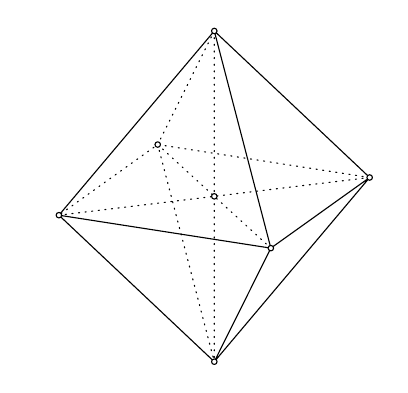
\begin{tikzpicture}[>=stealth, line join=round, line cap=round, font=\footnotesize, scale=.7]
				\def\a{3}
				\def\b{1}
				\def\gA{20}
				\path
				(0:0) coordinate (O)
				(0:\a) arc (0:\gA:{\a} and {\b}) coordinate (A)
				arc (\gA:\gA+90:{\a} and {\b}) coordinate (B)
				arc (\gA+90:\gA+180:{\a} and {\b}) coordinate (C)
				arc (\gA+180:\gA+270:{\a} and {\b}) coordinate (D)
				(O)+(90:\a) coordinate (E)
				(O)+(-90:\a) coordinate (F)
				;
				\draw[dotted]
				(E)--(F) (A)--(C) (B)--(D)
				(A)--(B)--(C) (E)--(B)--(F)
				;
				\draw
				(E)--(A)--(F) (E)--(C)--(F) (E)--(D)--(F)
				(C)--(D)--(A)
				;
				\foreach \x in {A,B,C,D,O,E,F} \draw[fill=white](\x) circle (.05);
			\end{tikzpicture}
		}
	}
\end{ex}
\begin{ex}%[2H1G3-3]
	(Chuyên Lào Cai-2020) Cho lăng trụ đều $ABC.A'B'C'$ có tất cả các cạnh bằnga. Gọi $S$ là điểm đối xứng của $A$ qua $BC'$. Thể tích khối đa diện $ABCSB'C'$ là
	\choice
	{\True $\dfrac{a^3\sqrt 3}{3}$}
	{$a^3\sqrt 3$}
	{$\dfrac{a^3\sqrt 3}{6}$}
	{$\dfrac{a^3\sqrt 3}{2}$}
	\loigiai{
		\immini{Chia khối đa diện $ABCSB'C'$ thành 2 khối là khối chóp $A.BCC'B'$ và khối chóp $S.BCC'B'$\\
			$V_{ABCSB'C'}=V_{ABCC'B'}+V_{S.BCC'B'}$\\
			Gọi $M$ là trung điểm $BC$.\\
			Ta có: $\left.\begin{array}{l}AM\perp BC\\AM\perp BB'\end{array}\right\}\Rightarrow AM\perp\left(BCC'B'\right)$.\\
			Tam giác $ABC$ đều $\Rightarrow AM=\dfrac{a\sqrt 3}{2}$.\\
			Thể tích khối chóp $ A.BCC'B'$ là:\\
			$V_{A.BCC'B'}=\dfrac{1}{3}AM.S_{BCC'B'}=\dfrac{1}{3}.\dfrac{a\sqrt 3}{2}.a^2=\dfrac{a^3\sqrt 3}{6}$.\\
			Thể tích khối chóp $ S.BCC'B'$ là:
			\allowdisplaybreaks
			\begin{eqnarray*}
				\dfrac{V_{S.BCC'B'}}{V_{A.BCC'B'}}&=&\dfrac{\dfrac{1}{3}d\left(S;\left(BCC'B'\right)\right).S_{BCC'B'}}{\dfrac{1}{3}d\left(A;\left(BCC'B'\right)\right).S_{BCC'B'}}\\
				&=&\dfrac{d\left(S;\left(BCC'B'\right)\right)}{d\left(A;\left(BCC'B'\right)\right)}=\dfrac{SI}{AI}=1.
			\end{eqnarray*}
			$\Rightarrow{V_{S.BCC'B'}}=V_{A.BCC'B'}=\dfrac{a^3\sqrt 3}{6}$\\
			$\Rightarrow{V_{ABCSB'C'}}=V_{A.BCC'B'}+V_{S.BCC'B'}=\dfrac{a^3\sqrt 3}{6}+\dfrac{a^3\sqrt 3}{6}=\dfrac{a^3\sqrt 3}{3}$
		}{
			\begin{tikzpicture}[line join=round, line cap=round,>=stealth,thick,scale=0.7]
				\coordinate (A) at (0,0);
				\coordinate (B) at ($(A) + (3,-3)$);
				\coordinate (C) at ($(A) + (5,0)$);
				\coordinate (A') at ($(A) + (0,4)$);
				\coordinate (B') at ($(B) + (0,4)$);
				\coordinate (C') at ($(C) + (0,4)$);
				\coordinate (Tempt) at ($(B)!(A)!(C')$);
				\coordinate (S) at ($(Tempt)!-1!(A)$);
				\coordinate (I) at ($(A)!0.5!(S)$);
				\coordinate (M) at ($(B)!0.5!(C)$);
				\fill[color=gray!35](B)--(B')--(C')--(C)--cycle;
				\foreach \i in {A,B,C,A',B',C',S,I,M}{\fill[black](\i) circle (1.5pt);}
				\foreach \i in {A,B,A',B'}{\draw(\i) node[scale=0.9, left]{$\i$};}
				\foreach \i in {C,C',S,M}{\draw(\i) node[scale=0.9, right]{$\i$};}
				\foreach \i in {I}{\draw(\i) node[scale=0.9, above right]{$\i$};}
				\draw(A)--(B) (B)--(S) (A)--(A') (A)--(B') (B)--(B') (A)--(A') (A')--(C') (B')--(C') (B')--(S) (C')--(S) (A')--(B');
				\draw[dashed](A)--(C) (A)--(S) (A)--(M) (B)--(C) (C)--(C') (B)--(C') (C)--(S) (A)--(C');
				\draw[dashed] pic[draw,angle radius=0.2cm]{right angle=A--M--C};
				\draw[dashed] pic[draw,angle radius=0.2cm]{right angle=A--I--C'};
			\end{tikzpicture}
		}
	}
\end{ex}

\begin{ex}%[2H1G3-2]
	(Chuyên Lê Hồng Phong-Nam Định-2020) Cho hình hộp $ ABCD.A'B'C'D'$ có đáy $ABCD$ là hình thoi tâm $O$, cạnh bằng $a$ và $\widehat{BAC}=60^\circ$. Gọi $I$, $J$ lần lượt là tâm của các mặt bên $ABB'A',CDD'C'$. Biết $AI=\dfrac{a\sqrt 7}{2}$, $ AA'=2a$ và góc giữa hai mặt phẳng $\left(ABB'A'\right),\left(A'B'C'D'\right)$ bằng $60^\circ$. Tính theo $a$ thể tích khối tứ diện $AOIJ$.
	\choice
	{$\dfrac{3\sqrt 3a^3}{64}$}
	{$\dfrac{\sqrt 3a^3}{48}$}
	{\True $\dfrac{\sqrt 3a^3}{32}$}
	{$\dfrac{\sqrt 3a^3}{192}$}
	\loigiai{
		\immini{
			Ta có $ A{I^2}=\dfrac{A{A'^2}+A{B^2}}{2}-\dfrac{A'{B^2}}{4}$\\
			$\Rightarrow A'{B^2}=2\left(A{A'^2}+A{B^2}\right)-4A{I^2}=3a^2\Rightarrow A'B=a\sqrt 3 $\\
			Do $ A'{B^2}+A{B^2}=A{A'^2}$ nên tam giác $ A'AB$vuông tại B$\Rightarrow{S_{A'AB}}=\dfrac{a^2\sqrt 3}{2}$\\
			Tam giác ABC đều cạnh a nên $S_{ABC}=\dfrac{a^2\sqrt 3}{4}$\\
			Theo đề góc giữa hai mặt phẳng $\left(ABB'A'\right),\left(A'B'C'D'\right)$ bằng $60^\circ$,\\
			nên suy ra $V_{A'ABC}=\dfrac{2S_{A'AB}.S_{ABC}\sin{60^\circ}}{3AB}=\dfrac{a^3\sqrt 3}{8}$
			\allowdisplaybreaks
			\begin{eqnarray*}
				V_{AOIJ}&=&\dfrac{1}{3}d\left(O;\left(IAJ\right)\right).S_{IAJ}\\
				&=&\dfrac{1}{3}.\dfrac{1}{2}d\left(B;\left(B'AD\right)\right).\dfrac{1}{2}{S_{B'AD}}\\
				&=&\dfrac{1}{4}{V_{B'ABD}}=\dfrac{1}{4}{V_{A'ABC}}=\dfrac{a^3\sqrt 3}{32}
			\end{eqnarray*}
		}{
			\begin{tikzpicture}[line join=round, line cap=round,>=stealth,thick,scale=0.65]
				\coordinate (A) at (0,0);
				\coordinate (B) at ($(A) + (-2,-2)$);
				\coordinate (C) at ($(B) + (5,0)$);
				\coordinate (D) at ($(A) + (5,0)$);
				\coordinate (A') at ($(A) + (1.5,4)$);
				\coordinate (B') at ($(B) + (1.5,4)$);
				\coordinate (C') at ($(C) + (1.5,4)$);
				\coordinate (D') at ($(D) + (1.5,4)$);
				\coordinate (O) at ($(A)!0.5!(C)$);
				\coordinate (I) at ($(A)!0.5!(B')$);
				\coordinate (J) at ($(C)!0.5!(D')$);
				\foreach \i in {A,B,C,D,A',B',C',D',O,I,J}{\fill[black](\i) circle (1.5pt);}
				\foreach \i in {A',B',C'}{\draw(\i) node[scale=0.9, above left]{$\i$};}
				\foreach \i in {A,C,D,D'}{\draw(\i) node[scale=0.9,below right]{$\i$};}
				\foreach \i in {I}{\draw(\i) node[scale=0.9, left]{$\i$};}
				\foreach \i in {J}{\draw(\i) node[scale=0.9, right]{$\i$};}
				\foreach \i in {B,O}{\draw(\i) node[scale=0.9,below left]{$\i$};}
				\draw(B')--(B) (B')--(A') (B')--(C') (B)--(B) (A')--(D') (C')--(D') (C')--(C) (C)--(D) (C)--(D') (C)--(D) (C)--(D') (B)--(C) (D)--(D') (C')--(D);
				\draw[dashed](A)--(B) (A)--(B') (A)--(A') (A)--(D) (A)--(C) (B)--(A') (B)--(D) (I)--(O) (I)--(J) (J)--(O);
			\end{tikzpicture}
		}
		\textit{\textbf{Bổ sung:} Công thức tính nhanh thể tích tứ diện theo góc giữa hai mặt phẳng}\\
		Cho tứ diện $ABCD$ có diện tích tam giác $ABC$ bằng $S_1$, diện tích tam giác $BCD$ là $S_2$và góc giữa hai mặt phẳng $(ABC)$ và $(DBC)$ là $\varphi $. Khi đó ta có: $V_{ABCD}=\dfrac{2S_1S_2.\sin\varphi}{3BC}$\\
		\immini{
			\textit{Chứng minh:} Gọi $H$ là hình chiếu của $A$ lên $(BCD)$, kẻ $HI \bot BC$ tại $I$ thì $AI \bot BC$ và $\left(\left(ABC\right);\left(DBC\right)\right)=\left(AI;HI\right)=\widehat{AIH}=\varphi$; $ AH=AI\sin\varphi $
			\allowdisplaybreaks
			\begin{eqnarray*}
				V_{ABCD}&=&\dfrac{1}{3}AH.S_{DBC}=\dfrac{1}{3}AI\sin\varphi \cdot S_2\\&=&\dfrac{1}{3}\dfrac{2S_{ABC}}{BC} \cdot \sin\varphi \cdot S_2=\dfrac{2S_1S_2\sin\varphi}{3BC}.
			\end{eqnarray*}
		}{
			\begin{tikzpicture}[line join=round, line cap=round,>=stealth,thick,scale=0.9]
				\coordinate (D) at (0,0);
				\coordinate (B) at ($(D) + (4,0)$);
				\coordinate (C) at ($(D) + (3,-1.5)$);
				\coordinate (A) at ($(D) + (2,2.5)$);
				\foreach \i in {A,B,C,D}{\fill[black](\i) circle (1.5pt);}
				\foreach \i in {A,D}{\draw(\i) node[scale=0.9,above left]{$\i$};}
				\foreach \i in {B,C}{\draw(\i) node[scale=0.9,below right]{$\i$};}
				\draw[dashed](B)--(D);
				\draw(A)--(D) (A)--(B) (A)--(C) (D)--(C) (B)--(C);
				\coordinate (H) at ($(A) + (0,-3)$);
				\coordinate (I) at ([scale around={0.3:(C)}] B);
				\foreach \i in {H,I}{\fill[black](\i) circle (1.5pt);}
				\foreach \i in {H}{\draw(\i) node[scale=0.9, left]{$\i$};}
				\foreach \i in {I}{\draw(\i) node[scale=0.9,right]{$\i$};}
				\draw[dashed](A)--(H) (H)--(I);
				\draw(A)--(I);
				\draw[dashed] pic[draw,angle radius=0.2cm]{right angle=A--H--I};
				\draw[dashed] pic[draw,angle radius=0.2cm]{right angle=C--I--H};
				\draw pic["$\varphi$",draw,angle eccentricity=1.9,angle radius=0.2cm]{angle=A--I--H};
			\end{tikzpicture}
		}
	}
\end{ex}

\begin{ex}%[2H1G3-2]
	(Chuyên Quang Trung-2020) Cho hình chóp $ S.ABCD$ đáy là hình vuông cạnh $a$, $SA$ vuông góc với mặt phẳng $\left(ABCD\right)$, $SA=a$. $ M,K$ tương ứng là trọng tâm tam giác $SAB,SCD$; $ N$ là trung điểm $ BC$. Thể tích khối tứ diện $SMNK$ bằng $\dfrac{m}{n}.a^3$với . Giá trị $m+n$ bằng:
	\choice
	{\True $28$}
	{$12$}
	{$19$}
	{$32$}
	\loigiai{
		\immini{
			Ta có: $V_{S.ABCD}=\dfrac{1}{3}SA.S_{ABCD}=\dfrac{a^3}{3}$.\\
			Gọi $ I$ là trung điểm của $ AB$, $ J$ là trung điểm của $ CD$.\\
			Ta có: $\Delta SMN$ đồng dạng với $\Delta SIJ$ theo tỉ số $\dfrac{2}{3}$.\\
			Do đó $V_{SMNK}=V_{P.SMN}=\left(\dfrac{2}{3}\right)^2V_{P.SIJ}=\dfrac{4}{9}{V_{P.SIJ}}$.\\
			Mặt khác $S_{\Delta PIJ}=\dfrac{1}{4}{S_{ABCD}}$.\\
			Do đó $V_{P.SIJ}=V_{S.PIJ}=\dfrac{1}{4}{V_{S.ABCD}}=\dfrac{a^3}{12}$\\
			Nên $V_{SMNK}=\dfrac{4}{9}.\dfrac{a^3}{12}=\dfrac{a^3}{27}$.\\
			Vậy $ m=1,n=27\Rightarrow m+n=28$.
		}{
			\begin{tikzpicture}[line join=round, line cap=round,>=stealth,thick,scale=0.7]
				\coordinate (A) at (0,0);
				\coordinate (D) at ($(A) + (6,0)$);
				\coordinate (V) at (-4,-2);
				\coordinate (B) at ($(A) + (V)$);
				\coordinate (C) at ($(D) + (V)$);
				\coordinate (S) at ($(A) + (0,4)$);
				\foreach \i in {A,B,C,D}{\fill[black](\i) circle (1.5pt);}
				\foreach \i in {A,B,C,D}{\draw(\i) node[scale=0.9,below right]{$\i$};}
				\foreach \i in {S}{\fill[black](\i) circle (1.5pt);}
				\foreach \i in {S}{\draw(\i) node[scale=0.9,above]{$\i$};}
				\draw[dashed](A)--(S) (A)--(B) (A)--(D);
				\draw(S)--(B) (S)--(C) (S)--(D) (B)--(C) (C)--(D);
				\coordinate (I) at ($(B)!0.5!(A)$);
				\coordinate (M) at ([scale around={0.66666666:(S)}] I);
				\coordinate (J) at ($(C)!0.5!(D)$);
				\coordinate (K) at ([scale around={0.66666666:(S)}] J);
				\coordinate (N) at ($(C)!0.5!(B)$);
				\foreach \i in {M,N,K,I,J}{\fill[black](\i) circle (1.5pt);}
				\foreach \i in {M,I}{\draw(\i) node[scale=0.9,above left]{$\i$};}
				\foreach \i in {N}{\draw(\i) node[scale=0.9,below]{$\i$};}
				\foreach \i in {K}{\draw(\i) node[scale=0.9,right]{$\i$};}
				\foreach \i in {J}{\draw(\i) node[scale=0.9,below right]{$\i$};}
				\draw[dashed](S)--(I) (M)--(K) (I)--(J) (N)--(K) (M)--(N);
				\draw(S)--(J) (S)--(N);
			\end{tikzpicture}
		}
	}
\end{ex}

\begin{ex}%[2H1G3-2]
	(Chuyên Quang Trung-2020) Cho hình lăng trụ đứng$\,ABCD.A'B'C'D'$có đáy là hình thoi có cạnh $4a$ , $A'A=8a$ , $\widehat{BAD}=120^^\circ$. Gọi $M,N,K$ lần lượt là trung điểm cạnh $AB',B'C,BD'$ . Thể tích khối da diện lồi có các đỉnh là các điểm $A,B,C,M,N,K$ là:
	\choice
	{\True $ 12\sqrt 3\,a^3$}
	{$\dfrac{28\sqrt 3}{3}\,a^3$}
	{$ 16\sqrt 3\,a^3$}
	{$\dfrac{40\sqrt 3}{3}\,a^3$}
	\loigiai{
		\immini{
			$ MN//AC;\,MN=\dfrac{1}{2}AC$, $MNCA$ là hình thang.\\
			$V_{MNKABC}=V_{K.MNCA}+V_{B.MNCA}$\\
			$DK$ cắt $(B’AC)$ tại $B’$, $\dfrac{B'K}{B'D}=\dfrac{1}{2}$\\
			$\Rightarrow\dfrac{d\left(K;(MNCA)\right)}{d\left(D;(MNCA)\right)}=\dfrac{1}{2}$\\
			$\Rightarrow{V_{K.MNCA}}=\dfrac{1}{2}{V_{D.MNCA}}$\\
			Mà: $V_{B.MNCA}=V_{D.MNCA}$ nên ta có\\ $V_{MNKABC}=\dfrac{1}{2}{V_{B.MNCA}}+V_{B.MNCA}=\dfrac{3}{2}{V_{B.MNCA}}$\\
			Mặt khác: $S_{MNCA}=\dfrac{3}{4}{S_{B'AC}}$
			\allowdisplaybreaks
			\begin{eqnarray*}
				\Rightarrow{V_{B.MNCA}}&=&\dfrac{3}{4}{V_{B.B'AC}}=\dfrac{3}{4}{V_{B'.ABC}}\\
				&=&\dfrac{3}{4}\cdot \dfrac{1}{6}{V_{ABCD.A'B'C'D'}}=8\sqrt 3a^3
			\end{eqnarray*}
			$V_{MNKABC}=\dfrac{3}{2}{V_{B.MNCA}}=\dfrac{3}{2}8\sqrt 3\,a^3=12\sqrt 3\,a^3$.
		}{
			\begin{tikzpicture}[line join=round, line cap=round,>=stealth,thick,scale=0.5]
				\coordinate (D) at (0,0);
				\coordinate (V) at (0,5.6);
				\coordinate (C) at ($(D) + (3,-2)$);
				\coordinate (A) at ($(D) + (9,1)$);
				\coordinate (B) at ($(C) + (9,1)$);
				\coordinate (A') at ($(A) + (V)$);
				\coordinate (B') at ($(B) + (V)$);
				\coordinate (C') at ($(C) + (V)$);
				\coordinate (D') at ($(D) + (V)$);
				\coordinate (O) at ($(A)!0.5!(C)$);
				\foreach \i in {A,B,C,D,A',B',C',D'}{\fill[black](\i) circle (1.5pt);}
				\foreach \i in {A,B}{\draw(\i) node[scale=0.9,right]{$\i$};}
				\foreach \i in {C,C',D,D'}{\draw(\i) node[scale=0.9, below left]{$\i$};}
				\foreach \i in {A',B'}{\draw(\i) node[scale=0.9, above right]{$\i$};}
				\draw[dashed](A)--(B) (A)--(C) (A)--(D) (A)--(A');
				\draw(A')--(B') (B')--(C) (A')--(D') (B)--(B') (C)--(C') (D)--(D') (B)--(C) (C)--(D) (B')--(C')--(D');
				\coordinate (M) at ($(A)!0.5!(B')$);
				\coordinate (N) at ($(C)!0.5!(B')$);
				\coordinate (K) at ($(B)!0.5!(D')$);
				\foreach \i in {M,N,K}{\fill[black](\i) circle (1.5pt);}
				\foreach \i in {K}{\draw(\i) node[scale=0.9, above]{$\i$};}
				\foreach \i in {N}{\draw(\i) node[scale=0.9, below]{$\i$};}
				\foreach \i in {M}{\draw(\i) node[scale=0.9, right]{$\i$};}
				\draw[dashed](A)--(B') (B')--(C) (B')--(D);
				\draw[dashed](C)--(K) (B)--(N) (A)--(K) (M)--(K) (M)--(N) (M)--(B) (K)--(N);
			\end{tikzpicture}
		}
	}
\end{ex}

\begin{ex}%[2H1G3-3]
	\immini{
		(Chuyên Sơn La-2020) Cho hình chóp tứ giác đều $S.ABCD$ có cạnh đáy bằng a, cạnh bên hợp với đáy một góc $60^\circ$ . Gọi $M$ là điểm đối xứng của $C$ qua $D$, $N$ là trung điểm $SC$. Mặt phẳng $(BMN)$ chia khối chóp $S.ABCD$ thành hai phần (như hình vẽ bên). Tỉ số thể tích giữa hai phần $\dfrac{V_{SABFEN}}{V_{BFDCNE}}$ bằng\\
	}{\begin{tikzpicture}[line join=round, line cap=round,>=stealth,thick,scale=0.8]
			\coordinate (C) at (0,0);
			\coordinate (D) at ($(C) + (4,0)$);
			\coordinate (V) at (-2,-2);
			\coordinate (B) at ($(C) + (V)$);
			\coordinate (A) at ($(D) + (V)$);
			\coordinate (S) at ($(C) + (1,3)$);
			\foreach \i in {A,B,C,D}{\fill[black](\i) circle (1.5pt);}
			\foreach \i in {C,D}{\draw(\i) node[scale=0.9,above right]{$\i$};}
			\foreach \i in {A,B}{\draw(\i) node[scale=0.9,below left]{$\i$};}
			\foreach \i in {S}{\fill[black](\i) circle (1.5pt);}
			\foreach \i in {S}{\draw(\i) node[scale=0.9,above]{$\i$};}
			\draw(A)--(S)--(B) (A)--(B);
			\draw[dashed](C)--(D) (C)--(B) (C)--(S);
			\coordinate (M) at ($(D)!-1!(C)$);
			\coordinate (N) at ($(C)!0.5!(S)$);
			\coordinate (O) at ($(C)!0.5!(A)$);
			\coordinate (E) at (intersection of M--N and S--D);
			\coordinate (F) at (intersection of B--M and A--D);
			\foreach \i in {M,N,E,F}{\fill[black](\i) circle (1.5pt);}
			\foreach \i in {N,O}{\draw(\i) node[scale=0.9, left]{$\i$};}
			\foreach \i in {M}{\draw(\i) node[scale=0.9, right]{$\i$};}
			\foreach \i in {E}{\draw(\i) node[scale=0.9, above right]{$\i$};}
			\foreach \i in {F}{\draw(\i) node[scale=0.9, below right]{$\i$};}
			\draw[dashed](B)--(N) (N)--(E) (B)--(F) (A)--(C) (B)--(D)--(N) (S)--(O)--(F)--(D) (E)--(D)--(M);
			\draw(S)--(E) (A)--(F) (F)--(M) (M)--(E) (E)--(F);
	\end{tikzpicture}}
	\choice
	{\True $\dfrac{7}{5}$}
	{$\dfrac{7}{6}$}
	{$\dfrac{7}{3}$}
	{$\dfrac{7}{4}$}
	\loigiai{
		Ta có $N$ là trung điểm của $SO$, $D$ là trung điểm của $CM$ nên $E$ là trọng tâm tam giác $SCM$.\\
		Ký hiệu $h,S,V$ tương ứng là chiều cao, diện tích đáy và thể tích khối chóp $S.ABCD$ ta có\\
		$S_{BCM}=S\Rightarrow{V_{N.BCM}}=\dfrac{1}{3}\cdot \dfrac{h}{2}.S=\dfrac{V}{2}$ .\\
		Khi đó $\dfrac{V_{M.EDF}}{V_{M.NCB}}=\dfrac{ME}{MN} \cdot \dfrac{MD}{MC} \cdot \dfrac{MF}{MB}=\dfrac{2}{3} \cdot \dfrac{1}{2}\cdot \dfrac{1}{2}=\dfrac{1}{6}\Leftrightarrow{V_{M.EDF}}=\dfrac{V}{2}\cdot\dfrac{1}{6}=\dfrac{V}{12}$ .\\
		Như vậy $V_{BFDCNE}=\dfrac{V}{2}-\dfrac{V}{12}=\dfrac{5V}{12}\Rightarrow{V_{SABFEN}}=\dfrac{7V}{12}\Rightarrow\dfrac{V_{SABFEN}}{V_{BFDCNE}}=\dfrac{7}{5}$ .}
\end{ex}

\begin{ex}%[2H1G3-2]
	(Chuyên Thái Bình-2020) Cho hình chóp $S.ABCD$ có đáy là hình vuông cạnh $2\sqrt 2 $. Cạnh bên $SA$ vuông góc với đáy và $SA=3$. Mặt phẳng $\left(\alpha\right)$ qua $A$ và vuông góc với $SC$ cắt các cạnh $SB,SC,SD$ tại $M,N,P$. Tính thể tích mặt cầu ngoại tiếp tứ diện $CMNP$
	\choice
	{\True $\dfrac{32\pi}{3}$}
	{$\dfrac{64\sqrt 2\pi}{3}$}
	{$\dfrac{108\pi}{3}$}
	{$\dfrac{125\pi}{6}$}
	\loigiai{
		\immini{
			Ta có: $\heva{&SA\perp BC\\&AB\perp BC}\Rightarrow BC\perp\left(SAB\right)\Rightarrow BC\perp MA$.\\
			Lại có $MA\perp SC\Rightarrow MA\perp\left(SBC\right)\Rightarrow MA\perp MC\,\,\,\,(1)$ .\\
			Tương tự: $AP\perp PC\,\,\,\,(2).$\\
			Mặt khác $AN\perp NC\,\,\,\,(3)$.\\
			Gọi $I$ là trung điểm của $AC$, từ $(1)$ $(2)$ $(3)$ ta có\\
			$IN=IM=IC=IP\left(=IA\right)$.\\
			Suy ra mặt cầu ngoại tiếp $CMNP$ là mặt cầu tâm $I$, bán kính $IA$.\\
			$IA=\dfrac{AC}{2}=\dfrac{\sqrt{\left(2\sqrt 2\right)^2+\left(2\sqrt 2\right)^2}}{2}=2.$\\
			Thể tích khối cầu ngoại tiếp tứ diện $CMNP$ là:\\
			$V=\dfrac{4}{3}\pi{2^3}=\dfrac{32\pi}{3}$.
		}{
			\begin{tikzpicture}[line join=round, line cap=round,>=stealth,thick,scale=0.7]
				\coordinate (A) at (0,0);
				\coordinate (D) at ($(A) + (6,0)$);
				\coordinate (V) at (-1.5,-2);
				\coordinate (B) at ($(A) + (V)$);
				\coordinate (C) at ($(D) + (V)$);
				\coordinate (S) at ($(A) + (0,4)$);
				\foreach \i in {A,B,C,D}{\fill[black](\i) circle (1.5pt);}
				\foreach \i in {A,B,C,D}{\draw(\i) node[scale=0.9,below right]{$\i$};}
				\foreach \i in {S}{\fill[black](\i) circle (1.5pt);}
				\foreach \i in {S}{\draw(\i) node[scale=0.9,above]{$\i$};}
				\draw[dashed](A)--(S) (A)--(B) (A)--(D);
				\draw(S)--(B) (S)--(C) (S)--(D) (B)--(C) (C)--(D);
				\coordinate (M) at ($(B)!0.5!(S)$);
				\coordinate (N) at ([scale around={0.33333333:(S)}] C);
				\coordinate (P) at ($(S)!0.5!(D)$);
				\coordinate (I) at ($(C)!0.5!(A)$);
				\foreach \i in {M,N,I,P}{\fill[black](\i) circle (1.5pt);}
				\foreach \i in {M}{\draw(\i) node[scale=0.9,above left]{$\i$};}
				\foreach \i in {I}{\draw(\i) node[scale=0.9,below]{$\i$};}
				\foreach \i in {N,P}{\draw(\i) node[scale=0.9,above right]{$\i$};}
				\draw[dashed](S)--(I) (M)--(A)--(N) (C)--(A)--(P);
				\draw (C)--(M)--(N)--(P)--(C)--(N);
			\end{tikzpicture}
		}
	}
\end{ex}

\begin{ex}%[2H1G3-2]
	(Chuyên Thái Nguyên-2020) Cho hình chóp $ S.ABC$ có đáy $ ABC$ là tam giác vuông cân đỉnh $ B$, $ AB=4$, $ SA=SB=SC=12$. Gọi $ M,N,E$ lần lượt là trung điểm của $ AC,BC,AB$. Trên cạnh $ SB$ lấy điểm $ F$ sao cho $\dfrac{BF}{BS}=\dfrac{2}{3}$. Thể tích khối tứ diện $ MNEF$ bằng
	\choice
	{$\dfrac{8\sqrt{34}}{3}$}
	{$\dfrac{4\sqrt{34}}{3}$}
	{\True $\dfrac{8\sqrt{34}}{9}$}
	{$\dfrac{16\sqrt{34}}{9}$}
	\loigiai{
		\immini{
			Vì $SA=SB=SC$ nên hình chiếu của $S$ lên $\left(ABC\right)$ là tâm đường tròn ngoại tiếp $ABC$, suy ra $ SM\perp\left(ABC\right)$.\\
			Từ $ AB=4\Rightarrow AC=4\sqrt 2 $.\\
			Tam giác $ SAM$ vuông tại $ M$ nên\\
			$SM=\sqrt{S{A^2}-A{M^2}}=\sqrt{12^2-\left(2\sqrt 2\right)^2}=2\sqrt{34}$. Khi đó\\
			\allowdisplaybreaks
			\begin{eqnarray*}
				V_{S.ABC}&=&\dfrac{1}{3}\cdot S_{ABC} \cdot SM=\dfrac{1}{3}\cdot\dfrac{1}{2}\cdot AB^2\cdot SM\\
				&=&\dfrac{1}{3}\cdot\dfrac{1}{2}\cdot 4^2\cdot 2\sqrt{34}=\dfrac{16\sqrt{34}}{3}
			\end{eqnarray*}
			Suy ra thể tích
			\begin{eqnarray*}
				V_{MNEF}&=&\dfrac{1}{3}\cdot S_{MNE}\cdot d\left(F,\left(MNE\right)\right)\\
				&=&\dfrac{1}{3}\cdot\dfrac{1}{4}\cdot S_{ABC} \cdot\dfrac{2}{3}\cdot SM\\
				&=&\dfrac{1}{12}\cdot V_{S.ABC}=\dfrac{1}{12}\cdot\dfrac{32\sqrt{34}}{3}=\dfrac{8\sqrt{34}}{9}.
			\end{eqnarray*}
		}{
			\begin{tikzpicture}[line join=round, line cap=round,>=stealth,thick,scale=0.9]
				\coordinate (A) at (0,0);
				\coordinate (C) at ($(A) + (6,0)$);
				\coordinate (B) at ($(A) + (2,-1.5)$);
				\coordinate (S) at ($(A) + (3,3)$);
				\foreach \i in {S,B,C,A}{\fill[black](\i) circle (1.5pt);}
				\foreach \i in {S,A}{\draw(\i) node[scale=0.9,above left]{$\i$};}
				\foreach \i in {B,C}{\draw(\i) node[scale=0.9,below right]{$\i$};}
				\draw[dashed](C)--(A);
				\draw(S)--(A) (S)--(B) (S)--(C) (A)--(B)--(C);
				\coordinate (M) at ($(C)!0.5!(A)$);
				\coordinate (N) at ($(C)!0.5!(B)$);
				\coordinate (E) at ($(B)!0.5!(A)$);
				\coordinate (F) at ([scale around={0.66666666:(B)}] S);
				\foreach \i in {M,N,E,F}{\fill[black](\i) circle (1.5pt);}
				\foreach \i in {F}{\draw(\i) node[scale=0.9, left]{$\i$};}
				\foreach \i in {E}{\draw(\i) node[scale=0.9, below left]{$\i$};}
				\foreach \i in {M}{\draw(\i) node[scale=0.9, below]{$\i$};}
				\foreach \i in {N}{\draw(\i) node[scale=0.9, below right]{$\i$};}
				\draw[dashed](S)--(M)--(E)--(N)--(M)--(F);
				\draw(E)--(F)--(N);
			\end{tikzpicture}
		}
	}
\end{ex}
\begin{ex}%[2H1G3-2]
	[Nguyễn Huệ-Phú Yên-2020] Cho hình hộp $ABCD.A'B'C'D'$ có chiều cao $8$ và diện tích đáy bằng $11$. Gọi $M$ là trung điểm của $AA'$, $N$ là điểm trên cạnh $BB'$ sao cho $BN=3B'N$ và $P$ là điểm trên cạnh $CC'$ sao cho $6CP=5C'P$. Mặt phẳng $(MNP)$ cắt cạnh $DD'$ tại $Q$. Thể tích của khối đa diện lồi có các đỉnh là các điểm $A$, $B$, $C$, $D$, $M$, $N$, $P$ và $Q$ bằng
	\choice
	{$\dfrac{88}{3}$}
	{\True $42$}
	{$44$}
	{$\dfrac{220}{3}$}
	\loigiai{
		\immini{Cho hình lăng trụ như hình vẽ\\
			$V_{ABC.MNP}=\dfrac{1}{3}\left(\dfrac{AM}{AA'}+\dfrac{BN}{BB'}+\dfrac{CP}{CC'}\right)\cdot V_{ABC.A'B'C'}$.\\
			Chứng minh:\\
			$V_{ABC.MNP}=V_{N.ACB}+V_{N.ACPM}$\\
			$V_{N.ACB}=\dfrac{BN}{BB'}\cdot V_{B'.ACB}=\dfrac{BN}{BB'}\cdot \dfrac{1}{3}\cdot V_{ABC.A'B'C'}$\\
			$\dfrac{V_{N.ACPM}}{V_{B'.ACC'A'}}=\dfrac{S_{ACPM}}{S_{ACC'A'}}=\dfrac{\dfrac{1}{2}\cdot\left(CP+AM\right)}{AA'}=\dfrac{1}{2}\cdot\left(\dfrac{CP}{CC'}+\dfrac{AM}{AA'}\right)$.
		}{
			\begin{tikzpicture}[scale=0.75, font=\footnotesize, line join=round, line cap=round, >=stealth]
				\def \a{3}
				\path
				(0,0) coordinate (A)
				(\a,0) coordinate (C)
				(-40:0.7*\a) coordinate (B)
				(80:1.2*\a) coordinate (A')
				($(A')+(B)$) coordinate (B')
				($(A')+(C)$) coordinate (C')
				($(A)!0.5!(A')$) coordinate (M)
				($(B)!0.75!(B')$) coordinate (N)
				($(C)!5/11!(C')$) coordinate (P)
				;
				\draw  (A)--(B)--(C)--(C')--(A')--(B')--(C')(A)--(A')(B)--(B')(M)--(N)--(P);
				\draw [dashed] (A)--(C)(M)--(P);
				\foreach \x/\g in {A/180,B/-90,C/0,A'/180,B'/-30,C'/0,M/180,N/-30,P/0}\fill[black] (\x) circle (1pt)+(\g:.3)node{$\x$};
			\end{tikzpicture}
		}
		\noindent $\Rightarrow{V_{N.ACPM}}=\dfrac{1}{2}\cdot\left(\dfrac{CP}{CC'}+\dfrac{AM}{AA'}\right)\cdot\dfrac{2}{3}{V_{ABC.A'B'C'}}$\\
		Từ đó ta suy ra điều phải chứng minh.\\
		Bây giờ ta áp dụng vào giải bài toán.\\
		\immini{
			Ta có $\heva{&\left(ADD'A'\right)\parallel\left(BCC'B'\right)\\&MQ\subset(MNP)\cap\left(ADD'A'\right)\\&NP\subset(MNP)\cap\left(BCC'B'\right)}\Rightarrow NP\parallel MQ$. Tương tự ta cũng có $MN\parallel PQ$. Do đó $MNPQ$ là hình bình hành.\\
			Ta có $OI$ là đường trung bình của hai hình thang $AMPC$ và $BNQD$ suy ra $2OI=MA+PC=DQ+NB$ $\Rightarrow\dfrac{MA}{AA'}+\dfrac{PC}{CC'}=\dfrac{BN}{BB'}+\dfrac{DQ}{DD'}$\\
			Dựa vào hình vẽ ta chia khối lăng trụ làm hai phần khi cắt bởi mặt phẳng $\left(BDD'B'\right)$. Do đó $V_{A'D'B'.ADB}=V_{BD'C'.BDC}=44$.\\
			
		}{
			\begin{tikzpicture}[scale=0.75, font=\footnotesize, line join=round, line cap=round, >=stealth]
				\def \a{4}
				\path
				(0,0) coordinate (D)
				(\a,0) coordinate (C)
				(210:0.7*\a) coordinate (A)
				($(A)+(C)$) coordinate (B)
				(80:1.2*\a) coordinate (D')
				($(D')+(B)$) coordinate (B')
				($(D')+(C)$) coordinate (C')
				($(D')+(A)$) coordinate (A')
				($(A)!0.5!(A')$) coordinate (M)
				($(B)!0.8!(B')$) coordinate (N)
				($(C)!0.4!(C')$) coordinate (P)
				($(M)!0.5!(P)$) coordinate (I)
				($(N)!2!(I)$) coordinate (Q)
				($(D)!.5!(B)$) coordinate (O)
				($(D')!.5!(B')$) coordinate (O')
				;
				\draw  (A)--(B)--(C)--(C')--(D')--(A')--(B')--(C')(A)--(A')(B)--(B')(M)--(N)--(P)(A')--(C')(B')--(D');
				\draw [dashed] (A)--(C)(M)--(P)(D)--(D')(O)--(O')(Q)--(N)(D)--(A')(Q)--(P)(B)--(D)(A)--(D)--(C)(M)--(Q);
				\foreach \x/\g in {A/180,B/-90,C/0,A'/180,B'/-30,C'/0,M/180,N/20,P/0,D/-90,D'/160,O/-90,O'/80,I/-40,Q/-40}\fill[black] (\x) circle (1pt)+(\g:.3)node{$\x$};
			\end{tikzpicture}
		}
		\begin{eqnarray*}
			V_{ABCD.MNPQ}&=&V_{ABD.MNQ}+V_{BCD.NPQ}\\
			&=&\dfrac{1}{3}\left(\dfrac{MA}{AA'}+\dfrac{BN}{BB'}+\dfrac{DQ}{DD'}\right)\cdot V_{ABD.A'B'D'}+\dfrac{1}{3}\left(\dfrac{CP}{CC'}+\dfrac{BN}{BB'}+\dfrac{DQ}{DD'}\right)\cdot V_{BCD.B'C'D'}\\
			&=&\dfrac{1}{3}\left(\dfrac{MA}{AA'}+\dfrac{BN}{BB'}+\dfrac{DQ}{DD'}+\dfrac{CP}{CC'}+\dfrac{BN}{BB'}+\dfrac{DQ}{DD'}\right)\cdot\dfrac{1}{2}{V_{ABC.A'B'C'}}\\
			&=&\dfrac{1}{3\cdot2}\left[3\cdot\left(\dfrac{MA}{AA'}+\dfrac{CP}{CC'}\right)\right]\cdot V_{ABC.A'B'C'}\\
			&=&\dfrac{1}{2}\left(\dfrac{MA}{AA'}+\dfrac{CP}{CC'}\right)\cdot V_{ABC.A'B'C'}\\
			&=&\dfrac{1}{2}\left(\dfrac{1}{2}+\dfrac{5}{11}\right)\cdot88=42.
		\end{eqnarray*}
	}
\end{ex}

\begin{ex}%[2H1G3-2]
	[Nguyễn Trãi-Thái Bình-2020] Cho hình chóp $S.ABCD$ có đáy là hình vuông, mặt bên $(SAB)$ là một tam giác đều nằm trong mặt phẳng vuông góc với mặt đáy $(ABCD)$ và có diện tích bằng $\dfrac{27\sqrt 3}{4}$ (đvdt). Một mặt phẳng đi qua trọng tâm tam giác $SAB$ và song song với mặt đáy $(ABCD)$ chia khối chóp $S.ABCD$ thành hai phần. Tính thể tích $V$ của phần chứa điểm $S$.
	\choice
	{$V=8$}
	{$V=24$}
	{$V=36$}
	{\True $V=12$}
	\loigiai{
		\immini{
			Gọi $H$ là trung điểm $AB$. Do $\triangle SAB$ đều và $(SAB)\perp(ABCD)$ nên $SH\perp(ABCD)$.\\
			Ta có $S_{\triangle SAB}=\dfrac{A{B^2}\sqrt 3}{4}=\dfrac{27\sqrt 3}{4}$ $\Rightarrow AB=3\sqrt 3\Rightarrow SH=\dfrac{AB\sqrt 3}{2}=\dfrac{3\sqrt 3\cdot\sqrt 3}{2}=\dfrac{9}{2}$.
			\begin{eqnarray*}
				\Rightarrow{V_{S.ABCD}}&=&\dfrac{1}{3}\cdot S_{ABCD}\cdot SH=\dfrac{1}{3}.A{B^2}\cdot SH\\
				&=&\dfrac{1}{3}{\left(3\sqrt 3\right)^2}\cdot\dfrac{9}{2}=\dfrac{81}{2}\text{ (đvtt)}.
			\end{eqnarray*}
		}{
			\begin{tikzpicture}[scale=1, font=\footnotesize, line join=round, line cap=round, >=stealth]
				\def \a{3.5}
				\path
				(0,0) coordinate (A)
				(\a,0) coordinate (D)
				(210:0.6*\a) coordinate (B)
				($(B)+(D)$) coordinate (C)
				($(A)!0.5!(B)$) coordinate (H)
				($(C)!0.5!(D)$) coordinate (K)
				($(H)!1!90:(K)$) coordinate (S)
				($(S)!2/3!(H)$) coordinate (G)
				($(S)!2/3!(A)$) coordinate (M)
				($(S)!2/3!(B)$) coordinate (N)
				($(S)!2/3!(C)$) coordinate (P)
				($(S)!2/3!(D)$) coordinate (Q)
				;
				\draw  (S)--(B)--(C)--(D)--(S)--(C) (N)--(P)--(Q);
				\draw [dashed] (B)--(A)--(D)(A)--(C) (M)--(P)(N)--(M)--(Q)(S)--(A)(S)--(H);
				\foreach \x/\g in {A/160,B/180,C/-20,D/0,M/50,N/180,P/-10,Q/20,S/90,G/-30,H/-70}\fill[black] (\x) circle (1pt)+(\g:.3)node{$\x$};
			\end{tikzpicture}
		}
		\noindent Gọi $G$ là trọng tâm tam giác $SAB$, qua $G$ kẻ đường thẳng song song với $AB$, cắt $SA$ và $SB$ lần lượt tại $M$, $N$. Qua $N$ kẻ đường thẳng song song với $BC$ cắt $SC$ tại $P$, qua $M$ kẻ đường thẳng song song với $AD$ cắt $SD$ tại $Q$. Suy ra $(MNPQ)$ là mặt phẳng đi qua $G$ và song song với $(ABCD)$.\\
		Khi đó $\dfrac{SM}{SA}=\dfrac{SN}{SB}=\dfrac{SP}{SC}=\dfrac{SQ}{SD}=\dfrac{SG}{SH}=\dfrac{2}{3}$.\\
		Có $\dfrac{V_{S.MNP}}{V_{S.ABC}}=\dfrac{SM}{SA}\cdot\dfrac{SN}{SB}\cdot\dfrac{SP}{SC}=\left(\dfrac{2}{3}\right)^3=\dfrac{8}{27}$\\
		$\Rightarrow{V_{S.MNP}}=\dfrac{8}{27}{V_{S.ABC}}=\dfrac{8}{27}\cdot\dfrac{1}{2}{V_{S.ABCD}}=\dfrac{4}{27}{V_{S.ABCD}}$.\\
		Có $\dfrac{V_{S.MPQ}}{V_{S.ACD}}=\dfrac{SM}{SA}\cdot\dfrac{SP}{SC}\cdot\dfrac{SQ}{SD}=\left(\dfrac{2}{3}\right)^3=\dfrac{8}{27}$.\\
		$\Rightarrow{V_{S.MPQ}}=\dfrac{8}{27}{V_{S.ACD}}=\dfrac{8}{27}\cdot\dfrac{1}{2}{V_{S.ABCD}}=\dfrac{4}{27}{V_{S.ABCD}}$.\\
		$V_{S.MNPQ}=V_{S.MNP}+V_{S.MPQ}=\dfrac{4}{27}{V_{S.ABCD}}+\dfrac{4}{27}{V_{S.ABCD}}=\dfrac{8}{27}{V_{S.ABCD}}=\dfrac{8}{27}\cdot\dfrac{81}{2}=12$ (đvtt).
	}
\end{ex}

\begin{ex}%[2H1G3-2]
	[Tiên Du-Bắc Ninh-2020] Cho hai hình chóp tam giác đều có cùng chiều cao. Biết đỉnh của hình chóp này trùng với tâm của đáy hình chóp kia, mỗi cạnh bên của hình chóp này đều cắt một cạnh bên của hình chóp kia. Cạnh bên có độ dài bằng $a$ của hình chóp thứ nhất tạo với đường cao một góc $30^\circ$, cạnh bên của hình chóp thứ hai tạo với đường cao một góc $45^\circ$. Tính thể tích phần chung của hai hình chóp đã cho.
	\choice
	{$\dfrac{3\left(2-\sqrt 3\right){a^3}}{64}$}
	{$\dfrac{\left(2-\sqrt 3\right){a^3}}{32}$}
	{\True $\dfrac{9\left(2-\sqrt 3\right){a^3}}{64}$}
	{$\dfrac{27\left(2-\sqrt 3\right){a^3}}{64}$}
	\loigiai{
		\immini{
			Hai hình chóp $A.BCD$ và $A'.B'C'D'$ là hai hình chóp đều, có chung đường cao $AA'$, $A$ là tâm của tam giác $B'C'D'$ và $A'$ là tâm của tam giác $BCD$.\\
			Ta có $(BCD)\parallel\left(B'C'D'\right)$; $AB=AC=AD=a$; $\widehat{BAA'}=\alpha$; $\widehat{AA'B'}=\beta$.\\
			Do $AB$ cắt $A'B'$ tại $M$ nên $AB'\parallel A'B$.\\
			Gọi $N$ là giao điểm của $AC$ và $A'C'$; $P$ là giao điểm của $AD$ và $A'D'$.\\
			Tương tự ta có: $AC'\parallel A'C$, $AD'\parallel A'D$.\\
			Từ đó suy ra các cạnh của $\triangle BCD$ và $\triangle B'C'D'$ song song với nhau từng đôi một.\\
			Ta có\\
			$\heva{&\dfrac{MB}{MA}=\dfrac{A'B}{AB'}\\&\dfrac{NC}{NA}=\dfrac{A'C}{AC'}\\&
				AB'=AC';\,A'B=A'C}\Rightarrow\dfrac{MB}{MA}=\dfrac{NC}{NA}\Rightarrow MN\parallel BC$.
		}{
			\begin{tikzpicture}[scale=1, font=\footnotesize, line join=round, line cap=round, >=stealth]
				\def \a{4}
				\path
				(0,0) coordinate (B)
				(\a,0) coordinate (D)
				(-60:0.5*\a) coordinate (C)
				($(C)!0.5!(D)$) coordinate (b)
				($(B)!0.5!(C)$) coordinate (d)
				($(B)!2/3!(b)$) coordinate (A')
				($(B)!(A')!(D)$) coordinate (X)
				($(X)!1.6!90:(D)$) coordinate (A)
				($(A)!0.5!(A')$) coordinate (H)
				($(A)!0.5!(B)$) coordinate (M)
				($(A)!0.5!(C)$) coordinate (N)
				($(A)!0.5!(D)$) coordinate (P)
				($(A')!2!(M)$) coordinate (B')
				($(A')!2!(N)$) coordinate (C')
				($(A')!2!(P)$) coordinate (D')
				($(B')!0.5!(C')$) coordinate (d')
				($(D')!0.5!(C')$) coordinate (b')
				($(N)!0.5!(P)$) coordinate (m)
				;
				\draw  (M)--(B)--(C)--(D)--(P)--(D')-- (D')--(B')--(C')--(D')(N)--(C)(C')--(N)(M)--(B')(b')--(B')(d')--(D')(N)--(P)(M)--(N);
				\draw [dashed] (A)--(M)--(P)--(A)--(A') (b)--(B)--(D)--(d)(A)--(N)(M)--(A')--(P)(M)--(m)(N)--(A');
				\foreach \x/\g in {A/90,B/180,C/-20,D/0,A'/-90,B'/180,C'/80,D'/0,M/180,N/180,P/0,H/20}\fill[black] (\x) circle (1pt)+(\g:.3)node{$\x$};
			\end{tikzpicture}
		}
		\noindent Tương tự ta có $NP\parallel CD$ và $MP\parallel BD$.\\
		Suy ra $\triangle MNP$ là tam giác đều. Gọi $H$ là giao điểm của $OO'$ và $(MNP)$, $H$ là tâm của tam giác $MNP$.\\
		Trong tam giác $AA'D$ có $AA'=AD\cdot\cos\alpha=a\cdot\cos\alpha $. $(1)$\\
		Đặt $x=MH$. Hai tam giác $AHM$ và tam giác $A'HM$ vuông tại $H$ cho\\
		$\heva{&AH=MH.\cot\alpha=x\cot\alpha\\&A'H=MH\cdot\cot\beta=x\cot\beta
		}\Rightarrow AA'=x\left(\cot\alpha+\cot\beta\right)$. $(2)$\\
		Từ $(1)$ và $(2)$ suy ra $a.\cos\alpha=x\left(\cot\alpha+\cot\beta\right)\Leftrightarrow x=\dfrac{a.\cos\alpha}{\cot\alpha+\cot\beta}$.\\
		Tam giác $MNP$ đều có cạnh $MN=x\sqrt 3$ nên\\
		$S_{\triangle MNP}=\dfrac{M{N^2}\sqrt 3}{4}=\dfrac{3\sqrt 3x^2}{4}=\dfrac{3\sqrt 3}{4}\cdot\dfrac{a^2\cos^2\alpha}{\left(\cot\alpha+\cot\beta\right)^2}$.\\
		Phần chung của hai hình chóp $A.BCD$ và $A'.B'C'D'$ là hai hình chóp đỉnh $A$ và $A'$ có chung nhau mặt đáy là tam giác $MNP$. Do đó thể tích của nó là\\
		$V=\dfrac{1}{3}S_{\triangle MNP}\left(AH+A'H\right)=\dfrac{1}{3}S_{\triangle MNP}\cdot AA'=\dfrac{a^3\sqrt 3\cos^3\alpha}{4\left(\cot\alpha+\cot\beta\right)^2}$.\\
		Với $\alpha=30^\circ $ và $\beta=45^\circ$ thì $V=\dfrac{9a^3}{32\left(\sqrt 3+1\right)^2}=\dfrac{9\left(2-\sqrt 3\right){a^3}}{64}$.
	}
\end{ex}

\begin{ex}%[2H1G3-2]
	[Lương Thế Vinh-Hà Nội-2020] Cho hình chóp $S.ABCD$ có đáy $ABCD$ là hình bình hành có diện tích bằng $12a^2$; khoảng cách từ $S$ tới mặt phẳng $(ABCD)$ bằng $4a$. Gọi $L$ là trọng tâm tam giác $ACD$; gọi $T$ và $V$ lần lượt là trung điểm các cạnh $SB$ và $SC$. Mặt phẳng $(LTV)$ chia hình chóp thành hai khối đa diện, hãy tính thể tích của khối đa diện chứa đỉnh $S$.
	\choice
	{$\dfrac{20a^3}{3}$}
	{$8a^3$}
	{\True $\dfrac{28a^3}{3}$}
	{$\dfrac{32a^3}{3}$}
	\loigiai{
		\immini{
			$V=V_{S.ABCD}=\dfrac{1}{3}12a^2\cdot4a=16a^3$.\\
			Mặt phẳng $(LTV)$ cắt $AB$, $CD$ ở $M$ và $N$ sao cho $MN\parallel BC\parallel TV$.\\
			Đặt $V'=V_{S.ADNMTV}=V_{S.ABMN}+V_{S.TVMN}$.\\
			Ta có $V_{S.ADNM}=\dfrac{1}{3}V$.\\
			Xét khối chóp $S.MNCB$ có đáy là hình bình hành\\
			$a=\dfrac{SM}{SM}=1$; $b=\dfrac{SN}{SN}=1$; $c=\dfrac{SB}{ST}=2$; $d=\dfrac{SC}{SV}=2$.\\
			Khi đó\\
			$\dfrac{V_{S.TVMN}}{V_{S.MNBC}}=\dfrac{a+b+c+d}{4abcd}=\dfrac{3}{8}\Rightarrow{V_{S.TVMN}}=\dfrac{2}{3}V.\dfrac{3}{8}=\dfrac{1}{4}V$.\\
			Do đó $V'=\dfrac{1}{3}V+\dfrac{1}{4}V=\dfrac{7}{12}V$ $=\dfrac{7}{12}\cdot16a^3=\dfrac{28}{3}{a^3}$.
		}{
			\begin{tikzpicture}[scale=0.8, font=\footnotesize, line join=round, line cap=round, >=stealth]
				\def \a{3.5}
				\path
				(0,0) coordinate (A)
				(\a,0) coordinate (D)
				(220:0.7*\a) coordinate (B)
				($(B)+(D)$) coordinate (C)
				(80:0.8*\a) coordinate (S)
				($(S)!0.5!(B)$) coordinate (T)
				($(S)!0.5!(C)$) coordinate (V)
				($(A)!1/3!(B)$) coordinate (M)
				($(D)!1/3!(B)$) coordinate (L)
				($(D)!1/3!(C)$) coordinate (N)
				;
				\draw  (S)--(B)--(C)--(D)--(S)--(C)(T)--(V)--(N);
				\draw [dashed] (B)--(A)--(D)(T)--(M)--(N) (A)--(C)(B)--(D)(S)--(A);
				\foreach \x/\g in {S/90,A/160,B/180,C/-20,D/0,T/150,V/50,M/-90,N/-10,L/-80}\fill[black] (\x) circle (1pt)+(\g:.3)node{$\x$};
			\end{tikzpicture}
		}
	}
\end{ex}

\begin{ex}%[2H1G3-2]
	[Thanh Chương 1-Nghệ An-2020] Cho hình chóp tứ giác đều $S.ABCD$ có thể tích bằng $1$. Gọi $M$ là trung điểm của $SA$ và $N$ là điểm đối xứng của của $A$ qua $D$ . Mặt phẳng $(BMN)$ chia khối chóp thành hai khối đa diện. Gọi $(H)$ là khối đa diện có chứa đỉnh. Thể tích của khối đa diện $(H)$ bằng
	\choice
	{\True $\dfrac{7}{12}$}
	{$\dfrac{4}{7}$}
	{$\dfrac{5}{12}$}
	{$\dfrac{3}{7}$}
	\loigiai{
		\immini{
			Gọi $O$ là tâm của hình vuông $ABCD$ ta có $SO$ là chiều cao của hình chóp.\\
			Trong mặt phẳng $(SAD)$ gọi $I$ là giao điểm của $MN$ và $SD$ ta suy ra $I$ là trọng tâm của tam giác $SAN$.\\
			Do đó $\dfrac{SI}{SD}=\dfrac{NI}{NM}=\dfrac{2}{3}$.\\
			Trong mặt phẳng $(ABCD)$ gọi $J$ là giao điểm của $BN$ và $CD$ ta suy ra $J$ là trung điểm của $CD$ và $BN$.
		}{
			\begin{tikzpicture}[scale=0.8, font=\footnotesize, line join=round, line cap=round, >=stealth]
				\def \a{3}
				\path
				(0,0) coordinate (A)
				(\a,0) coordinate (D)
				(210:0.7*\a) coordinate (B)
				($(B)+(D)$) coordinate (C)
				($(C)!0.5!(A)$) coordinate (O)
				($(A)!(O)!(D)$) coordinate (X)
				($(X)!1.4!90:(D)$) coordinate (S)
				($(S)!0.5!(A)$) coordinate (M)
				($(A)!2!(D)$) coordinate (N)
				($(D)!0.5!(C)$) coordinate (J)
				($(S)!2/3!(D)$) coordinate (I)
				;
				\draw  (S)--(B)--(C)--(J)--(I)--(S)--(C)(I)--(N)--(J);
				\draw [dashed] (B)--(A)--(D)--(J)(B)--(M)--(I) (A)--(C)(B)--(D)(C)--(A)--(S)--(O)(I)--(D)--(N)(B)--(J);
				\foreach \x/\g in {S/90,A/160,B/160,C/-20,D/40,I/60,J/-80,M/150,N/60,O/45}\fill[black] (\x) circle (1pt)+(\g:.3)node{$\x$};
			\end{tikzpicture}
		}
		\noindent Ta có $S_{\triangle ABN}=S_{ABCD}$ và $d(M,(ABCD))=\dfrac{1}{2}SO$ suy ra $V_{MABN}=\dfrac{1}{2}{V_{S.ABCD}}$. $(1)$\\
		Từ giả thiết ta có $V_{(H)}=V_{S.ABCD}-V_{ABM.DJI}$. $(2)$\\
		Xét trong khối chóp $N.ABM$ áp dụng công thức tính tỷ số thể tích ta có\\
		$\dfrac{V_{NDJI}}{V_{NABM}}=\dfrac{NI}{NM}\cdot\dfrac{ND}{NA}\cdot\dfrac{NJ}{NB}=\dfrac{1}{6}\Leftrightarrow{V_{NDJI}}=\dfrac{1}{6}{V_{NABM}}$.\\
		Do vậy $V_{ABM.DJI}=\dfrac{5}{6}{V_{NABM}}=\dfrac{5}{6}{V_{MABN}}$. $(3)$\\
		Từ $(1)$, $(2)$ và $(3)$ ta có thể tích của $(H)$ là\\
		$V_{(H)}=V_{S.ABCD}-\dfrac{5}{6}\cdot\dfrac{1}{2}{V_{S.ABCD}}=\dfrac{7}{12}$.\\
		Vậy thể tích của khối đa diện $(H)$ bằng $\dfrac{7}{12}$.
	}
\end{ex}

\begin{ex}%[2H1G3-2]
	[Tiên Lãng-Hải Phòng-2020]
	\immini{ Cho tứ diện $ABCD$ có thể tích $V$. Gọi $M$, $N$, $P$, $Q$, $R$ lần lượt là trung điểm của các cạnh $AB$, $AD$, $AC$, $DC$, $BD$ và $G$ là trọng tâm tam giác $ABC$ (như hình vẽ). Tính thể tích khối đa diện lồi $MNPQRG$ theo $V$.
		\choice
		{$\dfrac{V}{2}$}
		{$\dfrac{V}{6}$}
		{\True $\dfrac{V}{3}$}
		{$\dfrac{2V}{5}$}
	}{
		\begin{tikzpicture}[scale=1, font=\footnotesize, line join=round, line cap=round, >=stealth]
			\def \a{3.5}
			\path
			(0,0) coordinate (B)
			(\a,0) coordinate (D)
			(-60:0.5*\a) coordinate (C)
			(80:1.0*\a) coordinate (A)
			($(A)!0.5!(B)$) coordinate (M)
			($(A)!0.5!(D)$) coordinate (N)
			($(A)!0.5!(C)$) coordinate (P)
			($(B)!0.5!(D)$) coordinate (R)
			($(D)!0.5!(C)$) coordinate (Q)
			($(B)!0.5!(C)$) coordinate (K)
			($(A)!2/3!(K)$) coordinate (G)
			;
			\draw  (A)--(B)--(C)--(D)--(A)--(C)(M)--(P)--(N)--(Q)--(P)(M)--(G)--(P)(G)--(B);
			\draw [dashed] (B)--(D)(Q)--(G)--(R)--(Q)(M)--(N)--(R)(B)--(Q);
			\foreach \x/\g in {A/160,B/160,C/-20,D/40,M/160,N/60,P/-10,Q/-30,G/-90,R/45}\fill[black] (\x) circle (1pt)+(\g:.3)node{$\x$};
		\end{tikzpicture}
	}
	\loigiai{
		Ta có $V_{MNPQRG}=V_{G.MPQR}+V_{N.MPQR}$\\
		$V_{G.MPQR}=\dfrac{1}{3}{V_{B.MPQR}}=\dfrac{2}{3}{V_{B.PQR}}=\dfrac{2}{3}{V_{P.BQR}}=\dfrac{2}{3}\cdot\dfrac{1}{2}{V_{A.BQR}}=\dfrac{1}{3}\cdot\dfrac{1}{4}{V_{A.BCD}}=\dfrac{1}{12}V$.\\
		$V_{N.MPQR}=2V_{N.MPR}$ $=2\cdot V_{P.MNR}=2\cdot\dfrac{1}{2}{V_{C.MNR}}=\dfrac{1}{4}{V_{C.ABD}}=\dfrac{1}{4}V$.\\
		Vậy $V_{MNPQRG}=\dfrac{1}{12}V+\dfrac{1}{4}V=\dfrac{V}{3}$.
	}
\end{ex}

\begin{ex}%[2H1G3-2]
	[Trần Phú-Quảng Ninh-2020] Cho lăng trụ $ABC.A'B'C'$ có thể tích bằng $6$. Gọi $M$, $N$ và $P$ là các điểm nằm trên cạnh $A'B'$, $B'C'$ và $BC$ sao cho $M$ là trung điểm của $A'B'$, $B'N=\dfrac{3}{4}B'C'$ và $BP=\dfrac{1}{4}BC$. Đường thẳng $NP$ cắt đường thẳng $BB'$ tại $E$ và đường thẳng $EM$ cắt đường thẳng $AB$ tại $Q$. Thể tích của khối đa diện lồi $AQPCA'MNC'$ bằng
	\choice
	{$\dfrac{23}{3}$}
	{$\dfrac{23}{6}$}
	{\True $\dfrac{59}{12}$}
	{$\dfrac{19}{6}$}
	\loigiai{
		\immini{
			Ta có $\dfrac{EB}{EB'}=\dfrac{EQ}{EM}=\dfrac{EP}{EN}=\dfrac{BP}{B'N}=\dfrac{1}{3}$.\\
			Suy ra $\mathrm d\left(E,\left(A'B'C'\right)\right)=\dfrac{3}{2}\mathrm d\left(B,\left(A'B'C'\right)\right)$.\\
			Mà ta lại có $\dfrac{S_{B'MN}}{S_{A'B'C'}}=\dfrac{B'N}{B'C'}\cdot\dfrac{B'M}{B'A'}=\dfrac{3}{8}$.\\
			$V_{E.MB'N}=\dfrac{1}{3}\mathrm d\left(E,\left(MB'N\right)\right)\cdot S_{MB'N}=\dfrac{3}{16}{V_{ABC.A'B'C'}}=\dfrac{9}{8}$.\\
			Ta lại có $\dfrac{V_{E.QPB}}{V_{E.MNB'}}=\dfrac{EQ}{EM}\cdot\dfrac{EP}{EN}.\dfrac{EB}{EB'}=\left(\dfrac{EB}{EB'}\right)^3=\dfrac{1}{27}$.\\
			Suy ra $V_{BQP.B'MN}=V_{E.MB'N}-V_{EBQP}=\dfrac{26}{27}{V_{E.MB'N}}$.\\
			$V_{AQPCA'MNC'}=V_{ABC.A'B'C'}-V_{BQP.B'MN}=6-\dfrac{26}{27}\cdot\dfrac{9}{8}=\dfrac{59}{12}$.
		}{
			\begin{tikzpicture}[scale=1, font=\footnotesize, line join=round, line cap=round, >=stealth]
				\def \a{3.5}
				\path
				(0,0) coordinate (C')
				(\a,0) coordinate (B')
				(-60:0.5*\a) coordinate (A')
				(80:1.0*\a) coordinate (C)
				($(C)+(A')$) coordinate (A)
				($(C)+(B')$) coordinate (B)
				($(C)!0.75!(B)$) coordinate (P)
				($(A')!0.5!(B')$) coordinate (M)
				($(C')!0.25!(B')$) coordinate (N)
				(intersection of N--P and B'--B) coordinate (E)
				(intersection of M--E and A--B) coordinate (Q)
				;
				\draw  (C)--(C')--(A')--(B')--(E)--(M)(P)--(C)--(A)--(B)(E)--(P)(A)--(A')(Q)--(P);
				\draw [dashed] (C)--(N)--(P)--(B)(C')--(B')(A')--(N)--(M);
				\foreach \x/\g in {A/180,B/0,C/180,A'/200,B'/0,C'/180,M/-20,N/210,P/100,Q/-60,E/45}\fill[black] (\x) circle (1pt)+(\g:.3)node{$\x$};
			\end{tikzpicture}
		}
	}
\end{ex}
%%==========Câu 45
\begin{ex}%[2H1G3-3]
	[Sở Hà Tĩnh - 2021] Cho khối hộp $ABCD.A'B'C'D'$ có thể tích bằng $V$. Gọi $M$, $N$, $P$ lần lượt là trung điểm của $AB$, $B'C'$, $DD'$. Gọi thể tích khối tứ diện $CMNP$ là $V'$, khi đó tỉ số $\dfrac{V'}{V}$ bằng
	\choice
	{$\dfrac{1}{16}$}
	{\True $\dfrac{3}{16}$}
	{$\dfrac{1}{64}$}
	{$\dfrac{3}{64}$}
	\loigiai{
		\begin{center}
			\begin{tikzpicture}[scale=1.5, font=\footnotesize, line join=round, line cap=round, >=stealth]
				\def\bc{4} % cạnh BC
				\def\ba{2} % cạnh BA
				\def\h{4} % đường cao
				\def\gocB{35} % góc B của đáy
				\coordinate[label=below left:$B$] (B) at (0,0);
				\coordinate[label=above left:$A$] (A) at (\gocB:\ba);
				\coordinate[label=below:$C$] (C) at (\bc,0);
				\coordinate[label=right:$D$] (D) at ($(C)-(B)+(A)$);
				\coordinate[label=above left:$A'$] (A') at ($(A)+(90:\h)$);
				\coordinate[label=left:$B'$] (B') at ($(B)-(A)+(A')$);
				\coordinate[label=below right:$C'$] (C') at ($(C)-(A)+(A')$);
				\coordinate[label=right:$D'$] (D') at ($(D)-(A)+(A')$);
				\coordinate[label=left:$M$] (M) at ($(A)!0.5!(B)$);
				\coordinate[label=below left:$N$] (N) at ($(B')!0.5!(C')$);
				\coordinate[label=right:$P$] (P) at ($(D)!0.5!(D')$);
				\coordinate[label=below:$Q$] (Q) at ($(B)!0.5!(C)$);
				\coordinate[label=left:$H$] (H) at ($(A')!0.5!(B')$);
				\draw (B')--(B)--(C)--(D)--(D')--(A')--(B')--(C')--(D') (C)--(C') (Q)--(N)--(H)--(D')--(N)--(C)--(P);
				\draw[dashed,color=blue] (A')--(A)--(D) (A)--(B) (M)--(N)--(P)--(M)--(Q) (C)--(M)--(D) (P)--(H)--(M);
				\foreach \diem in {A,B,C,D,A',B',C',D',M,N,P,Q,H}	\fill (\diem)circle(1.5pt);
			\end{tikzpicture}
			
		\end{center}
		Ta có\\ $V=V'+V_{B'HN.BMQ}+V_{A'HD'.AMD}+V_{N.MQC}+V_{P.NCC'}+V_{P.D'C'N}+V_{P.D'HN}+V_{P.HNM}+V_{P.MDC}$.\\
		Gọi $S$ là diện tích đáy và $h$ là chiều cao khối hộp.\\
		Xét: $V_{B'HN.BMQ}=\dfrac{1}{8}Sh$, $V_{A'HD'.AMD}=\dfrac{1}{4}Sh$, $V_{N.MQC}=\dfrac{1}{24}Sh$, $V_{P.NCC'}=\dfrac{1}{12}Sh$,\\ $V_{P.D'C'N}=\dfrac{1}{24}Sh$, $V_{P.D'HN}=\dfrac{1}{16}Sh$, $V_{P.HNM}=V_{D'.HNM}=V_{M.HND'}=\dfrac{1}{8}Sh$, $V_{P.MDC}=\dfrac{1}{12}Sh$.\\
		Suy ra: $V=V'+\dfrac{13}{16}V\Leftrightarrow V'=\dfrac{3}{16}V\Leftrightarrow \dfrac{V'}{V}=\dfrac{3}{16}$.
	}
\end{ex}
%%==========Câu 46
\begin{ex}%[2H1G3-3]
	[Sở Tuyên Quang - 2021] Cho tứ diện $SABC$ và hai điểm $M$, $N$ lần lượt thuộc các cạnh $SA$, $SB$ sao cho $\dfrac{SM}{AM}=\dfrac{1}{2}$, $\dfrac{SN}{BN}=2$. Mặt phẳng $(P)$ đi qua hai điểm $M$, $N$ và song song với cạnh $SC$ cắt $AC$, $BC$ lần lượt tại $L$, $K$. Gọi $V$, $V'$ lần lượt là thể tích các khối đa diện $SCMNKL$, $SABC$. Tỉ số $\dfrac{V}{V'}$ bằng
	\choice
	{$\dfrac{2}{3}$}
	{\True $\dfrac{4}{9}$}
	{$\dfrac{1}{4}$}
	{$\dfrac{1}{3}$}
	\loigiai{
		\begin{center}
			\begin{tikzpicture}[scale=1.5, font=\footnotesize, line join=round, line cap=round, >=stealth]
				\def\ac{4} % cạnh AC
				\def\ab{2} % cạnh AB
				\def\as{4} % cạnh AS
				\def\gocA{50} % góc A của đáy
				\coordinate[label=left:$A$] (A) at (0,0);
				\coordinate[label=right:$C$] (C) at (\ac,0);
				\coordinate[label=below left:$B$] (B) at (-\gocA:\ab);
				\coordinate[label=above:$S$] (S) at (70:\as);
				\coordinate[label=left:$M$] (M) at ($(S)!1/3!(A)$);
				\coordinate[label=left:$N$] (N) at ($(S)!2/3!(B)$);
				\coordinate[label=above:$L$] (L) at ($(C)!1/3!(A)$);
				\coordinate[label=below right:$K$] (K) at ($(C)!2/3!(B)$);
				\coordinate[label=below:$I$] (I) at (intersection cs:first line={(M)--(N)}, second line={(L)--(K)});
				
				\draw (A)--(S)--(C)--(K)--(N)--(M) (A)--(I)--(N)--(B) (S)--(N) (I)--(K);
				\draw[dashed] (A)--(C) (B)--(K)--(L)--(M);
				\foreach \diem in {A,B,C,S,M,N,L,K,I}\fill (\diem)circle(1.5pt);
			\end{tikzpicture}
			
		\end{center}
		Gọi $I$ là giao điểm của $AB$, $MN$, $KL$.\\
		Do $ML$ $\parallel$ $SC$ và $NK$ $\parallel$ $SC$ nên ta có $\dfrac{AM}{AS}=\dfrac{AL}{AC}=\dfrac{2}{3}$ và $\dfrac{BN}{BS}=\dfrac{BK}{BC}=\dfrac{1}{3}$.\\
		Ta có $\dfrac{MA}{MS}\cdot \dfrac{NS}{NB}\cdot \dfrac{IB}{IA}=1$ suy ra $\dfrac{IB}{IA}=\dfrac{1}{4}$.\\
		Ta có $\dfrac{CL}{CA}\cdot \dfrac{BA}{BI}\cdot \dfrac{KI}{KL}=1\Leftrightarrow \dfrac{1}{3}\cdot \dfrac{3}{1}\cdot \dfrac{KI}{KL}=1\Leftrightarrow KL=KI$\\
		suy ra $MN=NI$ hay $\dfrac{IN}{IM}=\dfrac{IK}{IL}=\dfrac{1}{2}$.\\
		Xét hình chóp $IAML$ ta có $\dfrac{V_{I.BNK}}{V_{I.AML}}=\dfrac{IB\cdot IN\cdot IK}{IA\cdot IM\cdot IL}=\dfrac{1}{4}\cdot \dfrac{1}{2}\cdot \dfrac{1}{2}=\dfrac{1}{16}$.\\
		Mặt khác ta có $V_{IAML}=\dfrac{1}{3}d(I;(AML))\cdot{S_{\triangle AML}}=\dfrac{1}{3}\cdot \dfrac{4}{3}d(B;(AML))\cdot \dfrac{2}{3}\cdot \dfrac{2}{3}S_{\triangle SAC}=\dfrac{16}{27}V_{SABC}$.\\
		Suy ra $\dfrac{V_{I.BNK}}{V_{SABC}}=\dfrac{1}{16}\cdot \dfrac{16}{27}=\dfrac{1}{27}$.\\
		Suy ra $V_{I.BNK}=\dfrac{1}{27}\cdot V'\Rightarrow {V_{BNKAML}}=\dfrac{16}{27}V'-\dfrac{1}{27}\cdot V'=\dfrac{5}{9}V'$.\\
		Ta có $V_{SCMNKL}=V'-V_{BNKAML}=V'-\dfrac{5}{9}V'=\dfrac{4}{9}V'$.\\
		Từ đó ta có $\dfrac{V}{V'}=\dfrac{4}{9}$.}
\end{ex}
%%==========Câu 47
\begin{ex}%[2H1G3-3]
	[Liên trường Quỳnh Lưu - Hoàng Mai - Nghệ An - 2021] Cho lăng trụ $ABC.A'B'C'$. Gọi $M$, $N$, $Q$, $R$ lần lượt là trung điểm của các cạnh $AB$, $A'B'$, $BC$, $B'C'$ và $P$, $S$ lần lượt là trọng tâm của các tam giác $AA'B$, $CC'B$. Tỉ số thể tích khối đa diện $MNRQPS$ và khối lăng trụ $ABC.A'B'C'$ là
	\choice
	{$\dfrac{1}{9}$}
	{\True$\dfrac{5}{54}$}
	{$\dfrac{1}{10}$}
	{$\dfrac{2}{27}$}
	\loigiai{
		\textbf{(*) Cách 1:}
		\begin{center}
			\begin{tikzpicture}[scale=1.25, font=\footnotesize, line join=round, line cap=round, >=stealth]
				\def\ac{4} % cạnh AC
				\def\ab{2} % cạnh AB
				\def\ben{4} % cạnh bên
				\def\gocnghieng{75} % góc nghiêng cạnh bên
				\def\gocA{50} % góc A của đáy
				\coordinate[label=left:$A'$] (A') at (0,0);
				\coordinate[label=right:$C'$] (C') at (\ac,0);
				\coordinate[label=below left:$B'$] (B') at (-\gocA:\ab);
				\coordinate[label=left:$A$] (A) at ($(A')+(\gocnghieng:\ben)$);
				\coordinate[label=above:$B$] (B) at ($(B)-(A')+(A)$);
				\coordinate[label=right:$C$] (C) at ($(C)-(A')+(A)$);
				\coordinate[label=above:$M$] (M) at ($(A)!0.5!(B)$);
				\coordinate[label=below:$N$] (N) at ($(A')!0.5!(B')$);
				\coordinate[label=above:$Q$] (Q) at ($(B)!0.5!(C)$);
				\coordinate[label=right:$R$] (R) at ($(B')!0.5!(C')$);
				\coordinate[label=left:$P$] (P) at (intersection cs:first line={(A')--(M)}, second line={(A)--(B')});
				\coordinate[label=right:$S$] (S) at (intersection cs:first line={(Q)--(C')}, second line={(C)--(B')});
				\draw (A')--(A)--(B)--(C)--(C')--(B')--cycle (B)--(B') (N)--(M)--(Q)--(R) (M)--(A')--(B) (B')--(A)--(C) (Q)--(C')--(B);
				\draw[dashed] (A')--(C') (N)--(R)--(M);
				\foreach \diem in {A,B,C,A',B',C',M,N,Q,R,P,S} \fill (\diem)circle(1.5pt);
			\end{tikzpicture}
		\end{center}
		\begin{itemize}
			\item Đặt: $V=V_{ABC.A'B'C'}$; $V_{B'.AA'C'C}=\dfrac{1}{3}S_{AA'C'C}\cdot d\left(B',(AA'C'C)\right)=\dfrac{2}{3}V$.\\
			$\begin{aligned}[t]
				V_{B'.MNRQ}&=\dfrac{1}{3}\cdot{S_{MNRQ}}\cdot d\left(B',(MNRQ)\right)\\
				&=\dfrac{1}{3}\left(\dfrac{1}{2}S_{AA'C'C}\right)\cdot \left(\dfrac{1}{2}d\left(B',(AA'C'C)\right)\right)\\
				&=\left(\dfrac{1}{3}\cdot{S_{AA'C'C}}\cdot d\left(B',(AA'C'C)\right)\right)\cdot \dfrac{1}{4}\\
				&=\dfrac{1}{4}\cdot \dfrac{2}{3}V=\dfrac{1}{6}V.\end{aligned}$\\
			$V_{P.MNRQ}=\dfrac{1}{3}\cdot{V_{A'.MNRQ}}=\dfrac{1}{3}\cdot{V_{B'.MNRQ}}=\dfrac{1}{3}\cdot \dfrac{1}{6}V=\dfrac{1}{18}V$.
			\item $V_{A.BB'C'C}=\dfrac{1}{3}S_{BB'C'C}\cdot d\left(A,(BB'C'C)\right)=\dfrac{2}{3}V$.\\
			$S_{\triangle QRC'}=\dfrac{1}{2}S_{QRC'C}=\dfrac{1}{4}S_{BB'C'C}$;\\ $S_{\triangle QRS}=\dfrac{1}{3}S_{QRC'}=\dfrac{1}{3}\cdot \dfrac{1}{4}S_{BB'C'C}=\dfrac{1}{12}S_{BB'C'C}$.\\
			$\begin{aligned}[t]
				V_{A.QRS}&=\dfrac{1}{3}S_{\triangle QRS}\cdot d\left(A,(QRS)\right)\\
				&=\dfrac{1}{3}\left(\dfrac{1}{12}S_{BB'C'C}\right)\cdot \left(d\left(A,(BB'C'C)\right)\right)\\
				&=\left(\dfrac{1}{3}\cdot{S_{BB'C'C}}\cdot d\left(A,(BB'C'C)\right)\right)\cdot \dfrac{1}{12}\\
				&=\dfrac{1}{12}\cdot \dfrac{2}{3}V=\dfrac{1}{18}V.\end{aligned}$\\
			$V_{P.QRS}=\dfrac{PB'}{AB'}\cdot{V_{A.QRS}}=\dfrac{2}{3}\cdot \dfrac{1}{18}V=\dfrac{1}{27}V$.\\
			$V_{MNRQPS}=V_{P.MNRQ}+V_{P.QRS}=\dfrac{1}{18}V+\dfrac{1}{27}V=\dfrac{5}{54}V$.
		\end{itemize}
		Vậy: $\dfrac{V_{MNRQPS}}{V_{ABC.A'B'C'}}=\dfrac{5}{54}$.\\
		\textbf{(*) Cách 2:}
		\begin{center}
			\begin{tikzpicture}[scale=1.3, font=\footnotesize, line join=round, line cap=round, >=stealth]
				\def\ac{4} % cạnh AC
				\def\ab{2} % cạnh AB
				\def\h{4} % chiều cao
				\def\gocA{50} % góc A của đáy
				\coordinate[label=left:$A'$] (A') at (0,0);
				\coordinate[label=above right:$C'$] (C') at (\ac,0);
				\coordinate[label=below left:$B'$] (B') at (-\gocA:\ab);
				\coordinate[label=left:$A$] (A) at ($(A')+(90:\h)$);
				\coordinate[label=below left:$B$] (B) at ($(B')-(A')+(A)$);
				\coordinate[label=right:$C$] (C) at ($(C')-(A')+(A)$);
				\coordinate[label=above:$M$] (M) at ($(A)!0.5!(B)$);
				\coordinate[label=above:$Q$] (Q) at ($(B)!0.5!(C)$);
				\coordinate[label=left:$N$] (N) at ($(A')!0.5!(B')$);
				\coordinate[label=right:$R$] (R) at ($(B')!0.5!(C')$);
				\coordinate [label=right:$x$] (x) at ($(A')!1.5!(B')$);
				\coordinate [label=above:$y$] (y) at ($(A')!1.5!(C')$);
				\coordinate [label=left:$z$] (z) at ($(A')!1.3!(A)$);
				\draw[->] (B')--(x);
				\draw[->] (C')--(y);
				\draw[->] (A)--(z);
				\draw (A')--(A)--(B)--(C)--(C')--(B')--cycle (A)--(C) (B)--(B') (N)--(M)--(Q)--(R) (A')--(M) (Q)--(C');
				\draw (0,2)node[left]{$2$} (2,0)node[above]{$2$} (1,-1)node[below left]{$2$};
				\draw[dashed] (A')--(C') (N)--(R);
				\foreach \diem in {A,B,C,A',B',C',M,N,Q,R} \fill (\diem)circle(1.5pt);
			\end{tikzpicture}
		\end{center}
		\begin{itemize}
			\item Chuẩn hóa lăng trụ $ABC.A'B'C'$ là lăng trụ đứng có đáy $\triangle ABC$ vuông tại $A$ và các cạnh $AB=AC=AA'=2$.\\
			Khi đó: $V_{ABC.A'B'C'}=\left(\dfrac{1}{2}\cdot 2\cdot 2\right)\cdot 2=4$.\\
			Đặt khối lăng trụ $ABC.A'B'C'$ vào hệ trục tọa độ $Oxyz$ sao cho: $A'\equiv O$ và $B'$, $C'$, $A$ lần lượt nằm trên chiều dương của các trục $Ox$, $Oy$, $Oz$ (như hình vẽ).\\
			Ta có $A'(0;0;0)$, $B'(2;0;0)$, $C'(0;2;0)$, $A(0;0;2)$, $B(2;0;2)$, $C(0;2;2)$
			$M(1;0;2)$, $N(1;0;0)$, $R(1;1;0)$, $Q(1;1;2)$, $P\left(\dfrac{2}{3};0;\dfrac{4}{3}\right)$, $\overrightarrow{SC'}=-2\overrightarrow{SQ}$
			$\Rightarrow S=\left(\dfrac{2}{3};\dfrac{4}{3};\dfrac{4}{3}\right)$.\\
			$\overrightarrow{PM}=\left(\dfrac{1}{3};0;\dfrac{2}{3}\right)$, $\overrightarrow{PR}=\left(\dfrac{1}{3};1;-\dfrac{4}{3}\right)$, $\overrightarrow{PQ}=\left(\dfrac{1}{3};1;\dfrac{2}{3}\right)$, $\overrightarrow{PS}=\left(0;\dfrac{4}{3};0\right)$.\\
			$V_{P.MQR}=\dfrac{1}{6}\cdot \left| \left[\overrightarrow{PM};\overrightarrow{PQ}\right]\right|\cdot \overrightarrow{PR}=\dfrac{1}{6}\cdot \dfrac{2}{3}=\dfrac{1}{9}$;\\ $V_{P.MQRN}=2\cdot{V_{P.MQR}}=\dfrac{2}{9}$.\\
			$V_{P.QRS}=\dfrac{1}{6}\cdot \left| \left[\overrightarrow{PR};\overrightarrow{PQ}\right]\right|\cdot \overrightarrow{PS}=\dfrac{1}{6}\cdot \dfrac{8}{9}=\dfrac{4}{27}$.\\
			\item $V_{MNRQPS}=V_{P.MQRN}+V_{P.QRS}=\dfrac{2}{9}+\dfrac{4}{27}=\dfrac{10}{27}$.
		\end{itemize}
		Vậy: $\dfrac{V_{MNRQPS}}{V_{ABC.A'B'C'}}=\dfrac{\dfrac{10}{27}}{4}=\dfrac{5}{54}.$}
\end{ex}
%%==========Câu 48
\begin{ex}%[2H1G3-3]
	[Chuyên KHTN - 2021] Cho khối chóp tứ giác $S.ABCD$ có cạnh đáy bằng $a$ và cạnh bên bằng $2a$. Gọi $M$ là điểm đối xứng của $C$ qua $D$, $N$ là trung điểm của $SC$. Mặt phẳng $(BMN)$ chia khi chóp đã cho thành $2$ phần. Thể tích của phần chứa đỉnh $S$ bằng
	\choice
	{$\dfrac{3\sqrt{14}a^3}{32}$}
	{$\dfrac{5\sqrt{14}a^3}{72}$}
	{$\dfrac{7\sqrt{14}a^3}{96}$}
	{\True $\dfrac{7\sqrt{14}a^3}{72}$}
	\loigiai{
		\begin{center}
			\begin{tikzpicture}[scale=1.5, font=\footnotesize, line join=round, line cap=round, >=stealth]
				\def\bc{4} % cạnh BC
				\def\ba{2} % cạnh BA
				\def\h{4} % đường cao
				\def\gocB{30} % góc B của đáy
				\coordinate[label=below left:$B$] (B) at (0,0);
				\coordinate[label=above right:$C$] (C) at (\gocB:\ba);
				\coordinate[label=below:$A$] (A) at (\bc,0);
				\coordinate[label=above right:$D$] (D) at ($(C)-(B)+(A)$);
				\coordinate[label=above right:$O$] (O) at ($(A)!.5!(C)$);
				\coordinate[label=above:$S$] (S) at ($(O)+(90:\h)$);
				\coordinate[label=left:$N$] (N) at ($(S)!0.5!(C)$);
				\coordinate[label=above right:$M$] (M) at ($(C)!2!(D)$);
				\coordinate[label=above:$E$] (E) at (intersection cs:first line={(S)--(D)}, second line={(M)--(N)});
				\coordinate[label=below:$F$] (F) at (intersection cs:first line={(M)--(B)}, second line={(A)--(D)});
				\draw (B)--(A)--(F)--(E)--(S)--cycle (S)--(A) (E)--(M)--(F);
				\draw[dashed] (C)--(C)--(D)--(B) (O)--(S)--(C)--(B)--(N)--(E)--(D)--(F) (D)--(M) (B)--(F) (A)--(C);
				\foreach \diem in {A,B,C,D,S,O,M,N,E,F}	\fill (\diem)circle(1.5pt);
			\end{tikzpicture}
		\end{center}
		Giả sử các điểm như hình vẽ. $F=(BMN)\cap AD$; Kẻ $OH\perp SF$.\\
		Gọi $E=SD\cap MN\Rightarrow E$ là trọng tâm $\triangle SCM$, $DF\parallel BC\Rightarrow F$ là trung điểm $BM$.\\
		Ta có $SO=\sqrt{SD^2-DO^2}=\sqrt{(2a)^2-\left(\dfrac{a\sqrt{2}}{2}\right)^2}=\sqrt{4a^2-\dfrac{a^2}{2}}=\dfrac{a\sqrt{14}}{2}$.\\
		$\Rightarrow SF=\sqrt{SO^2+OF^2}=\sqrt{\left(\dfrac{a\sqrt{14}}{2}\right)^2+\left(\dfrac{a}{2}\right)^2}=\dfrac{a\sqrt{15}}{2}$.
		\begin{itemize}
			\item $d(M;(SBC))=4\cdot d(O;(SAD))=4OH=4\dfrac{SO\cdot OF}{SF}=\dfrac{2a\sqrt{210}}{15};\\
			S_{\triangle SAD}=\dfrac{1}{2}\cdot SF\cdot AD=\dfrac{a^2\sqrt{15}}{4}$.\\
			\item $\dfrac{V_{MEFD}}{V_{MNBC}}=\dfrac{ME}{MN}\cdot \dfrac{MF}{MB}\cdot \dfrac{MD}{MC}=\dfrac{2}{3}\cdot \dfrac{1}{2}\cdot \dfrac{1}{2}=\dfrac{1}{6}\Rightarrow {V_{MEFD}}=\dfrac{1}{6}\cdot{V_{MNBC}}$.
		\end{itemize}
		$\begin{aligned}[t]
			\Rightarrow {V_{BFDCNE}}&=\dfrac{5}{6}\cdot{V_{MNBC}}\\
			&=\dfrac{5}{6}\cdot \dfrac{1}{3}\cdot d(M;(SBC))\cdot \dfrac{1}{2}\cdot{S_{\triangle SBC}}\\
			&=\dfrac{5}{6}\cdot \dfrac{1}{3}\cdot 4OH\cdot \dfrac{1}{2}\cdot{S_{\triangle SAD}}=\dfrac{5a^3\sqrt{14}}{72}.\end{aligned}$\\
		Suy ra $V_{S.ABCD}=\dfrac{1}{3}\cdot SO\cdot{S_{ABCD}}=\dfrac{a^3\sqrt{14}}{6}\Rightarrow {V_{SABFEN}}=V_{S.ABCD}-V_{BFDCNE}=\dfrac{7a^3\sqrt{14}}{72}$.}
\end{ex}
%%==========Câu 49
\begin{ex}%[2H1G3-2]
	[Chuyên Quang Trung - Bình Phước - 2021]
	\immini{Cho hình lăng trụ $ABCD.A'B'C'D'$ đáy là hình bình hành. Với $AC=BC=a$, $CD=a\sqrt{2}$, $AC'=a\sqrt{3}$, $\widehat{CA'B'}=\widehat{A'D'C}=90^\circ$. Thể tích khối tứ diện $BCDA'$ là
		\choice
		{\True $\dfrac{a^3}{6}$}
		{$a^3$}
		{$\dfrac{2a^3}{3}$}
		{$\sqrt{6}a^3$}
	}{
		\begin{tikzpicture}[scale=.8, font=\footnotesize, line join=round, line cap=round, >=stealth]
			\def\bc{4} % cạnh BC
			\def\ba{2} % cạnh BA
			\def\h{4} % đường cao
			\def\gocB{45} % góc B của đáy
			\coordinate[label=below left:$D'$] (B') at (0,0);
			\coordinate[label=above left:$A'$] (A') at (\gocB:\ba);
			\coordinate[label=below:$C'$] (C') at (\bc,0);
			\coordinate[label=right:$B'$] (D') at ($(C')-(B')+(A')$);
			\coordinate (H) at ($(B')!0.4!(D')$); % Hình chiếu của A'
			\coordinate[label=above left:$A$] (A) at ($(H)+(122:\h)$);
			\coordinate[label=left:$D$] (B) at ($(B')-(A')+(A)$);
			\coordinate[label=below right:$C$] (C) at ($(C')-(A')+(A)$);
			\coordinate[label=right:$B$] (D) at ($(D')-(A')+(A)$);
			\draw (B)--(B') (C')--(D')--(D)--(A)--(B)--(C)--(D) (B')--(C')--(C) ;
			\draw[dashed] (A')--(D') (A)--(A')--(B') (A)--(A') ;
			\foreach \diem in {A,B,C,D,A',B',C',D'}	\fill (\diem)circle(1.5pt);
		\end{tikzpicture}
	}
	\loigiai{
		\begin{center}
			\begin{tikzpicture}[scale=.8, font=\footnotesize, line join=round, line cap=round, >=stealth]
				\def\bc{4} % cạnh BC
				\def\ba{2} % cạnh BA
				\def\h{4} % đường cao
				\def\gocB{45} % góc B của đáy
				\coordinate[label=below left:$D'$] (B') at (0,0);
				\coordinate[label=above left:$A'$] (A') at (\gocB:\ba);
				\coordinate[label=below:$C'$] (C') at (\bc,0);
				\coordinate[label=right:$B'$] (D') at ($(C')-(B')+(A')$);
				\coordinate (H) at ($(B')!0.4!(D')$); % Hình chiếu của A'
				\coordinate[label=above left:$A$] (A) at ($(H)+(122:\h)$);
				\coordinate[label=left:$D$] (B) at ($(B')-(A')+(A)$);
				\coordinate[label=below right:$C$] (C) at ($(C')-(A')+(A)$);
				\coordinate[label=right:$B$] (D) at ($(D')-(A')+(A)$);
				\coordinate[label=left:$O$] (O) at ($(A')!0.5!(C)$);
				\coordinate[label=below:$H$] (H) at ($(D')!2!(C')$);
				\draw (B)--(B') (C')--(D')--(D)--(A)--(B)--(C)--(D) (C')--(C)--(A) (C)--(H) (B')--(H)--(C');
				\draw[dashed] (A')--(D') (A)--(A')--(B') (A')--(C) (A)--(C')--(A') (B')--(C') (A')--(H);
				\foreach \diem in {A,B,C,D,A',B',C',D',O,H}	\fill (\diem)circle(1.5pt);
				\draw pic[angle radius=3mm,draw=blue,fill=green!50,opacity=.3,angle eccentricity=1.5] {right angle = C--H--C'};
				\draw pic[angle radius=3mm,draw=blue,fill=blue,opacity=.3,angle eccentricity=1.5] {right angle = C--H--B'};
			\end{tikzpicture}
		\end{center}
		Ta có tam giác $ABC$ vuông cân tại $C$.\\
		Gọi $O$ là trung điểm của $AC'\Rightarrow OC'=OA=\dfrac{a\sqrt{3}}{2}$.\\
		Gọi $H$ là chân đường cao hạ từ $C$ xuống mặt $(A'B'C'D')$.\\
		Ta có $\heva{&A'D'\perp CH \\& A'D'\perp D'C}\Rightarrow A'D'\perp HD'$.\\
		Lại có: $\heva{&A'B'\perp A'C \\&A'B'\perp CH}\Rightarrow A'B'\perp A'H$.\\
		Ta có $A'H\perp A'B'\Rightarrow \widehat{HA'B'}=90^\circ;\widehat{A'D'H}=90^\circ$. Tam giác $A'D'H$ vuông cân tại $D'$.\\
		Giả sử $CH=x\Rightarrow CA'=\sqrt{x^2+2a^2}$.\\
		$CC'^2=x^2+a^2$\\
		$C'O=\dfrac{CC'^2+C'A'^2}{2}-\dfrac{CA'^2}{4}\Leftrightarrow \dfrac{3a^2}{4}=\dfrac{x^2+a^2+a^2}{2}-\dfrac{x^2+2a^2}{4}=\dfrac{x^2+2a^2}{4}$.\\
		Suy ra $x^2+2a^2=3a^2\Rightarrow x=a=CH$.\\
		Vậy $V_{BCDA'}=\dfrac{1}{6}V_{ABCD.A'B'C'D}=\dfrac{1}{6}\cdot CH\cdot{S_{ABCD}}=\dfrac{a^3}{6}$.}
\end{ex}
%%==========Câu 50
\begin{ex}%[2H1G3-3]
	[THPT Hoàng Hoa Thám - Đà Nẵng - 2021] Cho hình hộp $ABCD.A'B'C'D'$. Gọi $G$ là trọng tâm của tam giác $ABD$. Mặt phẳng $(P)$ đi qua hai điểm $C'$, $G$ và song song với đường thẳng $BD$, chia khối hộp thành hai phần có thể thể tích $V_1$, $V_2$ $(V_1<V_2)$. Tỉ số $\dfrac{V_1}{V_2}$ bằng
	\choice
	{$\dfrac{V_1}{V_2}=\dfrac{1}{2}$}
	{$\dfrac{V_1}{V_2}=\dfrac{7}{17}$}
	{$\dfrac{V_1}{V_2}=\dfrac{2}{3}$}
	{\True $\dfrac{V_1}{V_2}=\dfrac{31}{77}$}
	\loigiai{
		\begin{center}
			\begin{tikzpicture}[scale=1.2, font=\footnotesize, line join=round, line cap=round, >=stealth]
				\def\bc{5} % cạnh BC
				\def\ba{2} % cạnh BA
				\def\h{4} % đường cao
				\def\gocB{45} % góc B của đáy
				\coordinate[label=below left:$A$] (A) at (0,0);
				\coordinate[label=above left:$B$] (B) at (\gocB:\ba);
				\coordinate[label=below:$D$] (D) at (\bc,0);
				\coordinate[label=right:$C$] (C) at ($(D)-(A)+(B)$);
				\coordinate (H) at ($(A')!0.4!(D)$); % Hình chiếu của A'
				\coordinate[label=above left:$B'$] (B') at ($(H)+(90:\h)$);
				\coordinate[label=left:$A'$] (A') at ($(A)-(B)+(B')$);
				\coordinate[label=right:$D'$] (D') at ($(D)-(B)+(B')$);
				\coordinate[label=right:$C'$] (C') at ($(C)-(B)+(B')$);
				\coordinate[label=below:$G$] (G) at ($(A)!1/3!(C)$);
				\coordinate[label=below:$J$] (J) at ($(B)!1/3!(A)$);
				\coordinate[label=below:$M$] (M) at ($(C)!4/3!(B)$);
				\coordinate[label=below:$N$] (N) at ($(C)!4/3!(D)$);
				\coordinate[label=below:$K$] (K) at (intersection cs:first line={(M)--(N)}, second line={(A)--(D)});
				\coordinate[label=right:$E$] (E) at (intersection cs:first line={(C')--(N)}, second line={(D')--(D)});
				\coordinate[label=above left:$F$] (F) at (intersection cs:first line={(B)--(B')}, second line={(C')--(M)});
				
				\draw (A')--(A)--(K) (D)--(C)--(C')--(B')--(A')--(D')--(C') (D)--(D') (C')--(N)--(K)--(E) (D)--(N);
				\draw[dashed] (C)--(B)--(A)--(C) (B')--(B)--(D) (C')--(M)--(K)--(D) (C')--(G) (M)--(B);
				\foreach \diem in {A,B,C,D,A',B',C',D',G,J,M,N,K,E,F}	\fill (\diem)circle(1.5pt);
			\end{tikzpicture}
		\end{center}
		\begin{itemize}
			\item Gọi $V$ là thể tích khối hộp $ABCD.A'B'C'D'$.\\
			Dựng $\Delta =(P)\cap (ABCD)$, ta có $\Delta \parallel BD$ (do $(P)\parallel BD$).\\
			Gọi $M$, $J$, $K$, $N$ lần lượt là giao điểm của $\Delta$ với $BC$, $AB$, $AD$, $DC$ và $F$, $E$ lần lượt là giao điểm của $MC'$ với $BB'$ và $NC'$ với $DD'$.
			\item Ta có $\dfrac{CM}{CB}=\dfrac{CN}{CD}=\dfrac{4}{3}$. Suy ra $S_{CMN}=\left(\dfrac{4}{3}\right)^2\cdot{S_{CBD}}=\dfrac{16}{9}S_{CBD}$.\\
			Mặt khác $\dfrac{JB}{JA}=\dfrac{JM}{JK}=\dfrac{1}{2}$. Suy ra $S_{JBM}=\left(\dfrac{1}{2}\right)^2\cdot{S_{JAK}}=\dfrac{1}{4}S_{JAK}$.\\
			Mà $\dfrac{AJ}{AB}=\dfrac{AK}{AD}=\dfrac{2}{3}$. Suy ra $S_{AJK}=\left(\dfrac{2}{3}\right)^2\cdot{S_{ABD}}=\dfrac{4}{9}S_{ABD}$.\\ Suy ra $S_{JBM}=\dfrac{1}{4}\cdot \dfrac{4}{9}S_{ABD}=\dfrac{1}{9}S_{ABD}$.\\
			\item Tương tự $S_{NKD}=\dfrac{1}{9}S_{ABD}$.\\
			\item Ta lại có $\dfrac{d\left(C',\left(ABCD\right)\right)}{d\left(F,\left(ABCD\right)\right)}=\dfrac{MC'}{MF}=4\Rightarrow h=d\left(C',\left(ABCD\right)\right)=4d\left(F,\left(ABCD\right)\right)$.\\
			\item Tương tự $h=d\left(C', (ABCD)\right)=4d\left(E, (ABCD)\right)$.\\
			\item Thể tích $\begin{aligned}[t]
				V_1&=V_{C'.CMN}-V_{F.MBJ}-V_{E.KDN}\\
				&=\dfrac{1}{3}\cdot \dfrac{16}{9}S_{BCD}\cdot h-2\cdot \dfrac{1}{3}\cdot \dfrac{1}{9}S_{BCD}\cdot \dfrac{1}{4}h\\
				&=\dfrac{31}{54}S_{BCD}\cdot h\\
				&=\dfrac{31}{108}S_{ABCD}\cdot h\\
				&=\dfrac{31}{108}V\Rightarrow V_2=\dfrac{77}{108}V.\end{aligned}$
		\end{itemize}
		Vậy $\dfrac{V_1}{V_2}=\dfrac{31}{77}$.}
\end{ex}
%%==========Câu 51
\begin{ex}%[2H1G3-3]
	[THPT Chu Văn An - Thái Nguyên - 2021] Cho khối lăng trụ đứng $ABC.A'B'C'$ có đáy tam giác vuông cân tại $C$. $BA=2a$ và góc tạo bởi $(ABC')$ và $(ABC)$ bằng $60^\circ$. Gọi $M$, $N$ lần lượt là trung điểm của $A'C'$ và $BC$. Mặt $(AMN)$ chia khối lăng trụ thành hai phần. Tìm thể tích phần nhỏ.
	\choice
	{\True $\dfrac{7\sqrt{3}a^3}{24}$}
	{$\dfrac{7\sqrt{6}a^3}{24}$}
	{$\dfrac{\sqrt{3}a^3}{3}$}
	{$\dfrac{\sqrt{6}a^3}{6}$}
	\loigiai{
		\begin{center}
			\begin{tikzpicture}[scale=1, font=\footnotesize, line join=round, line cap=round, >=stealth]
				\def\ac{4} % cạnh AC
				\def\ab{2} % cạnh AB
				\def\h{4} % chiều cao
				\def\gocA{50} % góc A của đáy
				\coordinate[label=left:$A$] (A) at (0,0);
				\coordinate[label=right:$C$] (C) at (\ac,0);
				\coordinate[label=below left:$B$] (B) at (-\gocA:\ab);
				\coordinate[label=left:$A'$] (A') at ($(A)+(90:\h)$);
				\coordinate[label=below right:$B'$] (B') at ($(B)-(A)+(A')$);
				\coordinate[label=right:$C'$] (C') at ($(C)-(A)+(A')$);
				\coordinate[label=above:$M$] (M) at ($(A')!0.5!(C')$);
				\coordinate[label=below:$N$] (N) at ($(B)!0.5!(C)$);
				\coordinate[label=left:$J$] (J) at ($(A)!0.5!(B)$);
				\coordinate[label=above:$P$] (P) at ($(C')!1/4!(B')$);
				\draw (A')--(A)--(B)--(C)--(C')--(A')--(B')--(C') (B)--(B') (M)--(P)--(N);
				\draw[dashed] (A)--(C) (A)--(M)--(N)--cycle (A')--(N) (C')--(J)--(C);
				\foreach \diem in {A,B,C,A',B',C',M,N,J,P} \fill (\diem)circle(1.5pt);
			\end{tikzpicture}
		\end{center}
		Kẻ $MP\parallel A'B'$\\
		Góc tạo bởi $(ABC')$ và $(ABC)$ là góc $\widehat{C'JC}=60^\circ$ với $J$ là trung điểm $AB$.\\
		$CC'=CJ\cdot \tan{60^\circ}=a\sqrt{3}$.\\
		$S_{ABC}=\dfrac{1}{2}CJ\cdot AB=a^2$.\\
		$S_1=S_{ACN}=\dfrac{1}{2}S_{ABC}=\dfrac{1}{2}a^2$.\\
		$S_2=S_{C'MP}=\dfrac{1}{4}S_{ABC}=\dfrac{1}{2}C'M\cdot C'P=\dfrac{1}{8}a^2$.\\
		$V=\dfrac{CC'}{3}(S_1+S_2+\sqrt{S_1S_2})=\dfrac{7\sqrt{3}a^3}{24}$.}
\end{ex}


\begin{ex}%[2H1K3-2]
	[THPT Ba Đình - Thanh Hóa - 2021]
	Cho hình lăng trụ $ABC.A'B'C'$ có thể tích bằng $2$. Gọi $M,N$ là các điểm lần lượt nằm trên các cạnh $AA',BB'$ sao cho $M$ là trung điểm của $AA'$ và $BN=\dfrac{1}{2}B'N$. Đường thẳng $CM$ cắt đường thẳng $A'C'$ tại điểm $P$, đường thẳng $CN$ cắt đường thẳng $A'B'$ tại $Q$. Tính thể tích của khối đa diện $A'MPB'NQ$ bằng.
	\choice
	{ $\dfrac{13}{18}$}
	{\True $\dfrac{23}{9}$}
	{ $\dfrac{21}{9}$}
	{ $\dfrac{7}{18}$}
	\loigiai{
		\begin{center}
			\begin{tikzpicture}[scale=1,font=\footnotesize,line join=round,line cap=round,>=stealth]
				\def\a{4}
				\def\h{4.5}
				\path 	(0:0) coordinate (A')
				++(0:\a) coordinate (C')
				++(-160:\a/2) coordinate (B')
				($(B')!0.5!(A')$) coordinate (H)
				($(C')!3/2!(H)$) coordinate (G)
				($(G)+(90:\h)$) coordinate (A)
				($(A)+(C')-(A')$) coordinate (C)
				($(C)+(B')-(C')$) coordinate (B)
				($(A)!0.5!(A')$) coordinate (M)
				($(B')!2/3!(B)$) coordinate (N)
				($(M)!1!180:(C)$) coordinate (P)
				($(N)!2!180:(C)$) coordinate (Q);
				\draw[dashed,thick] (A')--(C')  (A')--(B') (M)--(C) (A')--(P);
				\draw[thick] (C)--(C') 	(B)--(B') 	(A)--(A') (M)--(N) (P)--(M) (P)--(Q)--(B') (Q)--(C)
				(A)--(B)--(C)--cycle (B')--(C');
				\foreach \x/\g in {A/180,B/-145,C/0,A'/-150,B'/-45,C'/0,M/180,N/-45,P/90,Q/-90}
				\fill[black] 	(\x) circle (1pt)
				($(\g:4mm)+(\x)$) node {$\x$};
				%			\draw pic[draw,angle radius=2mm]{right angle=A'--G--C};%Theo chiều dương
			\end{tikzpicture}
		\end{center}
		Đặt $S={S_{\triangle A'B'C'}}$ và $h=d(C,(A'B'C'))$ ta có ${V_{ABC.A'B'C'}}=hS=2$.\\
		Trong mặt phẳng $\left( AA'C'C \right)$ ta có $\heva{
			& A'M=\dfrac{1}{2}CC' \\
			& A'M\subset CC' \\
		}$ nên ta có $A'$ là trung điểm của $PC'$.\\
		Tương tự trong mặt mặt phẳng $\left( BCC'B' \right)$ ta có $C'B'=\dfrac{1}{3}C'Q$.\\
		Từ đây ta có diện tích tam giác $C'PQ$ là ${S_{\triangle C'PQ}}=6S$ do vậy thể tích khối tứ diện $CC'PQ$ là $V_{CC'PQ}=\dfrac{1}{3}h\cdot 6S=2hS=4$.\\
		Trong khối lăng trụ $ABC.A'B'C'$ ta có $$\dfrac{V_{CABMN}}{V_{CAB.C'A'B'}}=\dfrac{1}{3}\left(\dfrac{AM}{A'M}+\dfrac{BN}{B'N}+\dfrac{CC}{CC'}\right)=\dfrac{\dfrac{1}{2}+\dfrac{1}{3}+0}{3}=\dfrac{5}{18}.$$
		Suy ra ${V_{CABMN}}=\dfrac{5}{18}.{V_{CAB.C'A'B'}}=\dfrac{5}{9}$ do đó thể tích khối $A'B'C'MNC$ bằng $2-\dfrac{5}{9}=\dfrac{13}{9}$.\\
		Do vậy thể tích của khối đa diện $A'MPB'NQ$ bằng $4-\dfrac{13}{9}=\dfrac{23}{9}$.}
\end{ex}
\begin{ex}%[2H1G3-2]
	[THPT Quốc Oai - Hà Nội - 2021]
	Cho hình chóp $S.ABC$ có đáy là tam giác đều cạnh $a$, mặt bên $SAB$ là tam giác đều và nằm trong mặt phẳng vuông góc với đáy. Gọi $H,M,O$ lần lượt là trung điểm các cạnh $AB$, $SA$, $AC$ và $G$ là trọng tâm tam giác $SBC$. Thể tích khối tứ diện $GHMO$ bằng
	\choice
	{ $\dfrac{3a^3}{64}$}
	{ $\dfrac{3a^3}{128}$}
	{ $\dfrac{a^3}{128}$}
	{\True $\dfrac{a^3}{64}$}
	\loigiai{
		\begin{center}
			\begin{tikzpicture}[scale=1,font=\footnotesize,line join=round,line cap=round,>=stealth]
				\def\a{5}
				\pgfmathsetmacro\h{\a*sqrt(3)/2}
				\path 	(0:0) coordinate (A)
				++(0:\a) coordinate (B)
				++(-140:4*\a/5) coordinate (C)
				($(A)!1/2!(B)$) coordinate (H)
				($(H)+(90:\h)$) coordinate (S)
				($(A)!1/2!(S)$) coordinate (M)
				($(A)!1/2!(C)$) coordinate (O)
				($(C)!1/2!(B)$) coordinate (N)
				($(S)!2/3!(N)$) coordinate (G)
				($(S)!1/2!(B)$) coordinate (E);
				\draw[thick,blue] (C)--(A) (E)--(C)--(B)
				(A)--(S)--(N)	(B)--(S)--(O)--(M)	(C)--(S);
				\draw[dashed,thick,red] (A)--(B) (S)--(H)--(M)--(G)--(H) (O)--(H)--(N)--(O);
				\foreach \x / \goc in 		{A/180,B/0,C/-135,H/-90,S/90,M/145,O/-135,G/45,N/-45,E/45}
				\fill (\x) circle (1.5pt)
				($(\x)+(\goc:3mm)$) node {$\x$};
				
				\draw pic[draw,angle radius=2mm]{right angle=A--H--S};%Theo chiều dương
			\end{tikzpicture}
		\end{center}
		Gọi $N,E$ lần lượt là trung điểm của $CB$ và $SB$.\\
		Ta có ${V_{S.ABC}}=\dfrac{1}{3}{S_{\triangle ABC}}\cdot SH=\dfrac{1}{3}\cdot\dfrac{a^2\sqrt{3}}{4}\cdot\dfrac{a\sqrt{3}}{2}=\dfrac{a^3}{8}$.\\
		+)${S_{OAHN}}=\dfrac{1}{2}{S_{\triangle ABC}}\Rightarrow {V_{S.OAHN}}=\dfrac{1}{2}{V_{S.ABC}}=\dfrac{a^3}{16}$, ${V_{S.AHN}}={V_{S.OAN}}=\dfrac{1}{2}{V_{S.AHNO}}=\dfrac{a^3}{32}$.\\
		+) $\dfrac{{V_{S.GMH}}}{{V_{S.NAH}}}=\dfrac{SG}{SN}.\dfrac{SM}{SA}\cdot\dfrac{SH}{SH}=\dfrac{2}{3}\cdot\dfrac{1}{2}=\dfrac{1}{3}\Rightarrow {V_{S.GMH}}=\dfrac{1}{3}{V_{S.NAH}}=\dfrac{a^3}{96}$.\\
		+) $\dfrac{{V_{S.GMO}}}{{V_{S.NAO}}}=\dfrac{SG}{SN}\cdot\dfrac{SM}{SA}\cdot\dfrac{SO}{SO}=\dfrac{2}{3}\cdot\dfrac{1}{2}=\dfrac{1}{3}\Rightarrow {V_{S.GMO}}=\dfrac{1}{3}{V_{S.NAO}}=\dfrac{a^3}{96}$.\\
		+) ${V_{G.ONH}}=\dfrac{1}{3}d\left( G,\left( ABC \right) \right)\cdot{S_{\triangle ONH}}=\dfrac{1}{3}\cdot\dfrac{1}{3}SH\cdot\dfrac{1}{4}{S_{\triangle ABC}}=\dfrac{1}{12}\cdot\dfrac{1}{3}SH\cdot{S_{\triangle ABC}}=\dfrac{1}{12}{V_{S.ABC}}=\dfrac{a^3}{96}$.\\
		+) ${V_{M.OAH}}=\dfrac{1}{3}d\left( M,\left( ABC \right) \right)\cdot{S_{\triangle OAH}}=\dfrac{1}{3}\cdot\dfrac{1}{2}SH\cdot\dfrac{1}{4}{S_{\triangle ABC}}=\dfrac{1}{8}\cdot\dfrac{1}{3}SH\cdot{S_{\triangle ABC}}=\dfrac{1}{8}{V_{S.ABC}}=\dfrac{a^3}{64}$.\\
		Vậy ${V_{GMOHN}}={V_{S.OAHN}}-{V_{S.GMH}}-{V_{S.GMO}}-{V_{G.HNO}}-{V_{G.HAO}}=\dfrac{a^3}{16}-3\cdot\dfrac{a^3}{96}-\dfrac{a^3}{64}=\dfrac{a^3}{64}$.}
\end{ex}
\begin{ex}%[2H1G3-2]
	[THPT Đồng Quan - Hà Nội - 2021]
	Cho lăng trụ đứng $ABC.A'B'C'$ có $AB=a$, $AC=2a$, $\widehat{BAC}=120^{\circ} $. Gọi $L$, $K$ lần lượt là tâm của các mặt bên $BCC'B'$, $ABB'A'$ và $E$ là trung điểm của $CC'$ (tham khảo hình vẽ).
	\begin{center}
		\begin{tikzpicture}[scale=1,font=\footnotesize,line join=round,line cap=round,>=stealth]
			\def\a{5}
			\def\h{4}
			\path 	(0:0) coordinate (B)
			++(0:\a) coordinate (C)
			++(-150:3*\a/4) coordinate (A)
			($(A)+(90:\h)$) coordinate (A')
			($(B)+(90:\h)$) coordinate (B')
			($(C)+(90:\h)$) coordinate (C')
			($(C)!1/2!(C')$) coordinate (E)
			($(A)!1/2!(B')$) coordinate (K)
			($(C)!1/2!(B')$) coordinate (L);
			\draw[dashed,thick,red] 	(C')--(B)--(C)--(B') (L)--(K)--(E)--(L);
			\draw[thick,blue]	(C)--(C') 	(B)--(B')--(A)	(A)--(A')--(B) (B)--(A)--(C) (A')--(B')--(C')--cycle;
			\foreach \x/\g in {A/-45,B/180,C/0,A'/-145,B'/-180,C'/0,E/0,K/145,L/90}
			\fill[black] 	(\x) circle (1pt)
			($(\g:4mm)+(\x)$) node {$\x$};
		\end{tikzpicture}
	\end{center}
	Biết hai mặt phẳng $\left( ACB' \right)$, $\left( ABC' \right)$ tạo với nhau một góc $\alpha $ thỏa mãn $\cos \alpha =\dfrac{\sqrt{10}}{5}$. Thể tích khối đa diện lồi có các đỉnh $A,B,C,K,E,I$ là.
	\choice
	{ $\dfrac{a^3}{2}$}
	{ $\dfrac{7a^3}{16}$}
	{ $\dfrac{5a^3}{8}$}
	{\True $\dfrac{9a^3}{16}$}
	\loigiai{
		\begin{center}
			\begin{tikzpicture}[scale=1,font=\footnotesize,line join=round,line cap=round,>=stealth]
				\def\a{5}
				\def\h{4}
				\path 	(0:0) coordinate (B)
				++(0:\a) coordinate (C)
				++(-150:3*\a/4) coordinate (A)
				($(A)+(90:\h)$) coordinate (A')
				($(B)+(90:\h)$) coordinate (B')
				($(C)+(90:\h)$) coordinate (C')
				($(C)!1/2!(C')$) coordinate (E)
				($(A)!1/2!(B')$) coordinate (K)
				($(C)!1/2!(B')$) coordinate (L)
				($(A)!2!-90:(B)$) coordinate (I')
				($(A)!1.5!(B)$) coordinate (Z)
				($ (A)!0.6!(I') $) coordinate (I);
				\draw[dashed,thick,red] 	(C')--(B)--(C)--(B') ;
				\draw[thick,blue]	(C)--(C') 	(B)--(B')--(A)	(A)--(A')--(B) (B)--(A)--(C) (A')--(B')--(C')--cycle;
				\draw[dashed] (C)--(I);
				\draw[->] (A')--($ (A')+(90:1) $)node[right]{$ z $};
				\draw[->] (B)--(Z)node[below left]{$ y $};
				\draw[dashed,->] (A)--(I')node[below right]{$ x $};
				\foreach \x/\g in {A/-45,B/180,C/0,A'/-180,B'/-180,C'/0,K/145,L/90,I/180}
				\fill[black] 	(\x) circle (1pt)
				($(\g:4mm)+(\x)$) node {$\x$};
			\end{tikzpicture}
			\begin{tikzpicture}[scale=1,font=\footnotesize,line join=round,line cap=round,>=stealth]
				\def\a{5}
				\def\h{4}
				\path 	(0:0) coordinate (B)
				++(0:\a) coordinate (C)
				++(-150:3*\a/4) coordinate (A)
				($(A)+(90:\h)$) coordinate (A')
				($(B)+(90:\h)$) coordinate (B')
				($(C)+(90:\h)$) coordinate (C')
				($(C)!1/2!(C')$) coordinate (E)
				($(A)!1/2!(B')$) coordinate (K)
				($(A)!1/2!(A')$) coordinate (H)
				($(B)!1/2!(B')$) coordinate (F)
				($(C)!1/2!(B')$) coordinate (L);
				\draw[dashed,thick,red] 	(C')--(B)--(C)--(B') (L)--(K)--(E)--(L)--(F);
				\draw[thick,blue]	(C)--(C') 	(B)--(B')--(A)	(A)--(A')--(B) (B)--(A)--(C) (A')--(B')--(C')--cycle (F)--(H)--(E)--(A);
				\foreach \x/\g in {A/-45,B/180,C/0,A'/-180,B'/-180,C'/0,E/0,K/182,L/90,H/45,F/180}
				\fill[black] 	(\x) circle (1pt)
				($(\g:4mm)+(\x)$) node {$\x$};
			\end{tikzpicture}
		\end{center}
		Kẻ tia $Ax$ vuông góc với $AB$ trên mặt phẳng $\left( ABC \right)$, chọn hệ trục tọa độ như hình vẽ.\\
		Gọi $I$ là hình chiếu của $C$ trên trục $Ax$, đặt $AA'=h$.\\
		Vì $ \widehat{BAC}=120^{\circ}=\widehat{IAB}+\widehat{IAC}=90^{\circ}+\widehat{IAC}
		\Rightarrow \widehat{IAC}=30^{\circ} $.\\
		Ta có $\widehat{IAC}=30^{\circ} \Rightarrow IC=AC\sin 30^{\circ} =a$, $IA=AC\cos 30^{\circ} =a\sqrt{3}$.\\
		Khi đó, trên hệ trục tọa độ đã chọn Ta có\\
		$A\left( 0;0;0 \right)$, $B\left( 0;a;0 \right)$, $C\left( a\sqrt{3};-a;0 \right)$, $B'\left( 0;a;h \right)$, $C'\left( a\sqrt{3};-a;h \right)$.\\
		+) $\overrightarrow{AC}=\left( a\sqrt{3};-a;0 \right),\overrightarrow{AB'}=\left( 0;a;h \right)\Rightarrow \left[ \overrightarrow{AC};\overrightarrow{AB'} \right]=\left( -ah;-ah\sqrt{3};a^2\sqrt{3} \right)$.\\
		Mặt phẳng $\left( ACB' \right)$ có VTPT $\overrightarrow{n_1}=\left( h;h\sqrt{3};-a\sqrt{3} \right)$.\\
		+) $\overrightarrow{AB}=\left( 0;a;0 \right),\overrightarrow{AC'}=\left( a\sqrt{3};-a;h \right)\Rightarrow \left[ \overrightarrow{AB};\overrightarrow{AC'} \right]=\left( ah;0;-a^2\sqrt{3} \right)$.\\
		Mặt phẳng $\left( ABC' \right)$ có VTPT $\overrightarrow{n_2}=\left( h;0;-a\sqrt{3} \right)$.\\
		Suy ra: $\cos \alpha =\left| \cos \left( \overrightarrow{n_1},\overrightarrow{n_2} \right) \right|\Leftrightarrow \dfrac{\sqrt{10}}{5}=\dfrac{\left| {h^2}+3a^2 \right|}{\sqrt{4h^2+3a^2}\sqrt{h^2+3a^2}}\Leftrightarrow \dfrac{\sqrt{10}}{5}=\dfrac{\sqrt{h^2+3a^2}}{\sqrt{4h^2+3a^2}}$\\
		$\Leftrightarrow \dfrac{2}{5}=\dfrac{h^2+3a^2}{4h^2+3a^2}\Leftrightarrow 8h^2+6a^2=5h^2+15a^2\Leftrightarrow h=a\sqrt{3}$.\\
		Gọi $V$ là thể tích khối đa diện lồi có các đỉnh $A,B,C,K,E,L$. Hai điểm $F,H$ lần lượt là trung điểm của $BB'$ và $AA'$.\\
		Ta có $\dfrac{{V_{B.FKL}}}{{V_{B.B'A'C'}}}=\dfrac{BF}{BB'}\cdot\dfrac{BK}{BA'}\cdot\dfrac{BL}{BC'}=\dfrac{1}{2}\cdot\dfrac{1}{2}\cdot\dfrac{1}{2}=\dfrac{1}{8}$.\\
		$\Rightarrow {V_{B.FKL}}=\dfrac{1}{8}{V_{B.B'A'C'}}=\dfrac{1}{8}\cdot\dfrac{1}{3}{V_{ABC.A'B'C'}}=\dfrac{1}{24}{V_{ABC.A'B'C'}}$.\\
		${V_{A.KHE}}=\dfrac{1}{3}AH\cdot{S_{HKE}}=\dfrac{1}{3}\cdot\dfrac{1}{2}AA'\cdot\dfrac{1}{2}{S_{HFE}}=\dfrac{1}{12}\cdot AA'\cdot{S_{HFE}}=\dfrac{1}{12}\cdot {V_{ABC.A'B'C'}}$.\\
		Vậy
		\begin{eqnarray*}
			V
			&=& {V_{ABC.HEF}}-{V_{A.HKE}}-{V_{B.FKL}}=\dfrac{1}{2}{V_{ABC.A'B'C'}}-\dfrac{1}{24}{V_{ABC.A'B'C'}}-\dfrac{1}{12}{V_{ABC.A'B'C'}}\\
			&=& \dfrac{3}{8}{V_{ABC.A'B'C'}}=\dfrac{3}{8}\cdot AA'\cdot\dfrac{1}{2}\cdot AB\cdot AC\sin 120^{\circ} =\dfrac{3}{8}\cdot h\cdot\dfrac{1}{2}\cdot AB\cdot AC\sin 120^{\circ} =\dfrac{9a^3}{16}.
		\end{eqnarray*}
	}
\end{ex}
\begin{ex}%[2H1K3-2]
	[Trung Tâm Thanh Tường -2021]
	Cho hình lăng trụ $ABC.A'B'C'$ có đáy ABC là tam giác đều cạnh bằng 2, $A'A=A'B=A'C=2$, M là trung điểm của $AA'$. Tính thể tích phần chung của 2 khối đa diện $A'M.BCC'B'$ và $A.A'B'C'$.\\
	\immini{
		\choice
		{\True $\dfrac{17\sqrt{2}}{27}$}
		{ $\dfrac{17\sqrt{3}}{18}$}
		{ $\dfrac{17\sqrt{3}}{27}$}
		{ $\dfrac{5\sqrt{2}}{3}$}}{
		\begin{tikzpicture}[scale=1,font=\footnotesize,line join=round,line cap=round,>=stealth]
			\def\a{4}
			\def\h{4.5}
			\path 	(0:0) coordinate (A)
			++(0:\a) coordinate (C)
			++(-135:\a/2) coordinate (B)
			($(B)!0.5!(C)$) coordinate (I)
			($(A)!2/3!(I)$) coordinate (H)
			($(H)+(90:\h)$) coordinate (A')
			($(A')+(C)-(A)$) coordinate (C')
			($(C')+(B)-(C)$) coordinate (B')
			($(A)!0.5!(A')$) coordinate (M);
			\draw[dashed,thick] (A)--(C) (M)--(C) (A)--(C');
			\draw[thick] (C)--(C') 	(B)--(B') 	(A)--(A') (B)--(M) (A)--(B')
			(A)--(B)--(C) (A')--(B')--(C')--cycle;
			\foreach \x/\g in {A/180,B/-45,C/0,A'/180,B'/-45,C'/0,M/180}
			\fill[black] 	(\x) circle (1pt)
			($(\g:4mm)+(\x)$) node {$\x$};
			%	\draw pic[draw,angle radius=2mm]{right angle=A'--G--C};%Theo chiều dương
	\end{tikzpicture}}
	
	\loigiai{
		\begin{center}
			\begin{tikzpicture}[scale=1,font=\footnotesize,line join=round,line cap=round,>=stealth]
				\def\a{4}
				\def\h{4.5}
				\path 	(0:0) coordinate (A)
				++(0:\a) coordinate (C)
				++(-135:\a/2) coordinate (B)
				($(B)!0.5!(C)$) coordinate (I)
				($(A)!2/3!(I)$) coordinate (H)
				($(H)+(90:\h)$) coordinate (A')
				($(A')+(C)-(A)$) coordinate (C')
				($(C')+(B)-(C)$) coordinate (B')
				($(A)!0.5!(A')$) coordinate (M);
				\path[name path=MB] (M)--(B);
				\path[name path=AB'] (A)--(B');
				\path[name intersections={of=MB and AB'}] (intersection-1) coordinate (P);
				\path[name path=MC] (M)--(C);
				\path[name path=AC'] (A)--(C');
				\path[name intersections={of=MC and AC'}] (intersection-1) coordinate (Q);
				\draw[dashed,thick] (A)--(C) (M)--(C) (I)--(A)--(C') (A')--(H);
				\draw[thick] (C)--(C') 	(B)--(B') 	(A)--(A') (B)--(M) (A)--(B')
				(A)--(B)--(C) (A')--(B')--(C')--cycle;
				\foreach \x/\g in {A/180,B/-45,C/0,A'/180,B'/-45,C'/0,H/45,M/180,I/-45,P/-90,Q/100}
				\fill[black] 	(\x) circle (1pt)
				($(\g:4mm)+(\x)$) node {$\x$};
				\draw pic[draw,angle radius=2mm]{right angle=I--H--A'};%Theo chiều dương
			\end{tikzpicture}
		\end{center}
		Gọi $ H $ là hình chiếu vuông góc của $A'$ lên mặt phẳng $ (ABC) $. Vì $A'A=A'B=A'C$ nên $ H $ trùng với tâm đường tròn ngoại tiếp tam giác $ ABC $ cũng là trọng tâm tam giác $ ABC $.\\
		Gọi $ I $ là trung điểm $ BC $.\\
		Ta có\\
		$AI=\sqrt{3}\Rightarrow AH=\dfrac{2}{3}AI=\dfrac{2\sqrt{3}}{3}$; $A'H=\sqrt{{AA'}^2-AH^2}=\sqrt{4-\dfrac{12}{9}}=\dfrac{2\sqrt{6}}{3}$;\\
		${V_{ABC.A'B'C'}}=A'H\cdot{S_{ABC}}=\dfrac{2\sqrt{6}}{3}\cdot\sqrt{3}=2\sqrt{2}$; ${V_{A.A'B'C'}}=\dfrac{1}{3}{V_{ABC.A'B'C'}}=\dfrac{2\sqrt{2}}{3}$;\\
		Gọi $P=AB'\cap BM$; $Q=AC'\cap CM$.\\
		Khi đó phần chung của 2 khối đa diện $A'M.BCC'B'$ và $A.A'B'C'$ là khối đa diện $MPQ.A'B'C'$.\\
		Ta có $\dfrac{{V_{A.MPQ}}}{{V_{A.A'B'C'}}}=\dfrac{AM}{AA'}\cdot\dfrac{AP}{AB'}\cdot\dfrac{AQ}{AC'}=\dfrac{1}{2}\cdot\dfrac{1}{3}\cdot\dfrac{1}{3}=\dfrac{1}{18}$\\
		$\Rightarrow {V_{MPQ.A'B'C'}}=\dfrac{17}{18}{V_{A.A'B'C'}}=\dfrac{17}{18}\cdot\dfrac{2\sqrt{2}}{3}=\dfrac{17\sqrt{2}}{27}$.}
\end{ex}
\begin{ex}%[2H1K3-2]
	[Trung Tâm Thanh Tường - 2021]
	Cho hình chóp $S.ABCD$ có đáy $ABCD$ là hình thang vuông tại $A$ và $B$, $AB=BC=a$, $AD=2a$, $SA$ vuông góc với đáy, $SA=a\sqrt{2}$. Gọi $B'$ là điểm đối xứng của $B$ qua mặt phẳng $\left( SCD \right)$. Tính thể tích khối đa diện $SB'.ABCD$ bằng
	\begin{center}
		\begin{tikzpicture}[scale=1,font=\footnotesize,line join=round,line cap=round,>=stealth]
			\def\a{4}
			\def\h{3.5}
			\path 	(0:0) coordinate (A)
			++(0:\a) coordinate (D)
			(-130:\a/2) coordinate (B)
			($ (B)+(0:\a/1.5) $) coordinate (C)
			($(A)+(90:\h)$) coordinate (S)
			($ (C)!0.5!(D) $) coordinate (C')
			($ (S)!2/3!(C') $) coordinate (B')
			(intersection of A--C and B--D) coordinate (O);%giao điểm O
			\draw[dashed,thick] 	(B)--(A)--(D)	(A)--(S) (C)--(S) ;
			\draw[thick] 			(B)-- (C)--(D)
			(B)--(S)--(B')--(C)		(B')--(D)--(S) (B)--(B');
			\foreach \x/\g in {A/135,B/-135,C/-45,D/45,S/90,B'/45}
			\fill[black] 	(\x) circle (1.5pt)
			($(\g:3mm)+(\x)$) node {$\x$};
			\draw pic[draw,angle radius=3mm]{right angle=D--A--S};%Theo chiều dương
		\end{tikzpicture}
	\end{center}
	\choice
	{ $\dfrac{5\sqrt{2}{a^3}}{6}$}
	{ $\dfrac{7\sqrt{2}{a^3}}{3}$}
	{ $\sqrt{2}{a^3}$}
	{\True $\dfrac{2\sqrt{2}{a^3}}{3}$}
	\loigiai{
		Ta có
		\begin{eqnarray*}
			{V_{SB'.ABCD}}
			&=& {V_{S.ABCD}}+{V_{B'SCD}}=\dfrac{1}{3}SA\cdot{S_{ABCD}}+\dfrac{1}{3}{S_{SCD}}\cdot d\left( B',\left( SCD \right) \right)\\
			&=& \dfrac{1}{3}SA\cdot{S_{ABCD}}+\dfrac{1}{3}{S_{SCD}}\cdot d\left( B,\left( SCD \right) \right).
		\end{eqnarray*}
		(vì $B'$ là điểm đối xứng của $B$ qua mặt phẳng $\left( SCD \right)$).
		\begin{center}
			\begin{tikzpicture}[scale=1,font=\footnotesize,line join=round,line cap=round,>=stealth]
				\def\a{4}
				\def\h{3.5}
				\path 	(0:0) coordinate (A)
				++(0:\a) coordinate (D)
				(-130:\a/2) coordinate (B)
				($ (B)+(0:\a/2) $) coordinate (C)
				($(A)+(90:\h)$) coordinate (S)
				($ (C)!0.5!(D) $) coordinate (C')
				($ (S)!2/3!(C') $) coordinate (B')
				($ (C)!0.5!(S) $) coordinate (H)
				(intersection of A--B and D--C) coordinate (M)
				(intersection of A--C and B--D) coordinate (O);%giao điểm O
				\draw[dashed,thick] 	(B)--(A)--(D)	(H)--(A)--(S) (A)--(C)--(S) ;
				\draw[thick] 			(B)-- (C)--(D) (B)--(M)--(C)
				(B)--(S)--(B')--(C)		(B')--(D)--(S) (B)--(B');
				\foreach \x/\g in {A/135,B/-180,C/-45,D/45,S/90,B'/45,M/145,H/45}
				\fill[black] 	(\x) circle (1.5pt)
				($(\g:3mm)+(\x)$) node {$\x$};
				\draw pic[draw,angle radius=2mm]{right angle=D--A--S};%Theo chiều dương
				\draw pic[draw,angle radius=3mm]{right angle=A--H--C};%Theo chiều dương
			\end{tikzpicture}
		\end{center}
		+ ${V_{S.ABCD}}=\dfrac{1}{3}SA.{S_{ABCD}}=\dfrac{1}{3}.a\sqrt{2}.\dfrac{\left( a+2a \right)a}{2}=\dfrac{a^3}{\sqrt{2}}$\\
		+ Gọi $M$ là giao điểm của $AB$ và $CD$, dễ dàng chứng minh được $B$ là trung điểm của $MA$.\\
		$\Rightarrow d\left( B,\left( SCD \right) \right)=\dfrac{1}{2}d\left( A,\left( SCD \right) \right)=\dfrac{1}{2}AH$.\\
		Lại có tam giác $SAC$ vuông cân tại $A$ ( vì $SA=AC=a\sqrt{2}$)\\
		$\Rightarrow d\left( B,\left( SCD \right) \right)=\dfrac{1}{2}d\left( A,\left( SCD \right) \right)=\dfrac{1}{2}AH=\dfrac{1}{4}SC=\dfrac{1}{4}\cdot 2a=\dfrac{a}{2}$.\\
		Ta có $ {V_{B'.SCD}}=\dfrac{1}{3}{S_{SCD}}\cdot d\left( B',\left( SCD \right) \right)=\dfrac{1}{3}\cdot\dfrac{1}{2}SC\cdot CD\dfrac{a}{2}=\dfrac{1}{6}\cdot 2a\cdot a\sqrt{2}\cdot\dfrac{a}{2}=\dfrac{a^3\sqrt{2}}{6}=\dfrac{a^3}{3\sqrt{2}}$\\
		${V_{SB'.ABCD}}={V_{S.ABCD}}+{V_{B'SCD}}=\dfrac{a^3}{\sqrt{2}}+\dfrac{a^3}{3\sqrt{2}}=\dfrac{2\sqrt{2}{a^3}}{3}$.}
\end{ex}
\begin{ex}%[2H1K3-2]
	[Chuyên Hà Tĩnh - 2021]
	Cho hình chóp $S.ABC$ có $SA$ vuông góc với mặt đáy, $SA=2BC=2a\sqrt{3}$, $AC=a$ và $\widehat{BAC}={{120}^{\text{o}}}$. Hình chiếu vuông góc của $A$ lên các cạnh $SB$ và $SC$ lần lượt là $M$ và $N$. Thể tích của khối đa diện $AMNCB$ bằng.
	\choice
	{ $\dfrac{24}{169}{a^3}$}
	{\True $\dfrac{25}{338}{a^3}$}
	{ $\dfrac{25}{169}{a^3}$}
	{ $\dfrac{12}{169}{a^3}$}
	\loigiai{
		\begin{center}
			\begin{tikzpicture}[scale=1,font=\footnotesize,line join=round,line cap=round,>=stealth]
				\def\a{4} %Khai báo cạnh
				\def\h{4}
				\path 	(0:0) coordinate (A)
				++(0:\a) coordinate (B)
				++(-140:4*\a/5) coordinate (C)
				($(A)+(90:\h)$) coordinate (S)
				($(S)!(A)!(B)$) coordinate (M)
				($(S)!(A)!(C)$) coordinate (N);;
				\draw[thick] 	(A)--(C)--(B)
				(M)--(N)--(A)--(S)	(B)--(S)	(C)--(S);
				\draw[dashed,thick] 	(M)--(A)--(B);
				\foreach \x /\goc in {A/180,B/0,C/-135,S/90,M/45,N/0}
				\fill[black] (\x) circle (1.5pt)
				($(\x)+(\goc:3mm)$) node {$\x$};
				\draw pic[draw,angle radius=2mm]{right angle=B--A--S};%Theo chiều dương
			\end{tikzpicture}
		\end{center}
		Có $SA=2BC=2a\sqrt{3}\Rightarrow SA=2a\sqrt{3};BC=a\sqrt{3}$.\\
		Xét $\triangle ABC$ có $\cos A=\dfrac{AB^2+AC^2-BC^2}{2AB\cdot AC}\Rightarrow -\dfrac{1}{2}=\dfrac{AB^2+a^2-3a^2}{2AB\cdot a}$.\\
		$\Rightarrow -a.AB=AB^2-2a^2\Leftrightarrow AB^2+a\cdot AB-2a^2=0\Leftrightarrow \left( AB-a \right)\left( AB+2a \right)=0$.\\
		$\Leftrightarrow \hoac{
			& AB=a \\
			& AB=-2a<0\left( KTM \right) \\
		}\Rightarrow AB=a$.\\
		Có ${V_{S.ABC}}=\dfrac{1}{3}SA\cdot{S_{ABC}}=\dfrac{1}{6}SA\cdot AB\cdot AC\sin \widehat{BAC}=\dfrac{a^3}{2}$.\\
		$\triangle SAB$ vuông tại $A$, đường cao $AM$.\\
		$\Rightarrow SA^2=SM.SB\Rightarrow SM=\dfrac{SA^2}{SB}=\dfrac{SA^2}{\sqrt{SA^2+A{B^2}}}=\dfrac{12a^2}{a\sqrt{13}}=\dfrac{12a}{\sqrt{13}}$.\\
		Tương tự, $SN=\dfrac{SA^2}{\sqrt{SA^2+A{C^2}}}=\dfrac{12a}{\sqrt{13}}$.\\
		Và $ SB=\sqrt{AB^2+AS^2}=\sqrt{a^2+(2a\sqrt{3})^2}=a\sqrt{13} $, $ SC=\sqrt{AC^2+AS^2}=\sqrt{a^2+(2a\sqrt{3})^2}=a\sqrt{13} $.\\
		Có $\dfrac{V_{SAMN}}{V_{SABC}}=\dfrac{SM}{SB}\cdot\dfrac{SN}{SC}=\dfrac{\dfrac{12a}{\sqrt{13}}}{a\sqrt{13}}\cdot\dfrac{\dfrac{12a}{\sqrt{13}}}{a\sqrt{13}}=\dfrac{144}{169}\Rightarrow \dfrac{V_{AMNCB}}{V_{SABC}}=\dfrac{25}{169}$.\\
		$\Rightarrow {V_{AMNCB}}=\dfrac{25}{169}{V_{SABC}}=\dfrac{25}{169}\cdot\dfrac{a^3}{2}=\dfrac{25a^3}{338}$.}
\end{ex}
\begin{ex}%[2H1K3-2]
	[Chuyên Long An - 2021]
	Cho hình chóp $S.ABCD$ có đáy là hình vuông cạnh $a$, $SA$ vuông góc với mặt đáy $\left( ABCD \right)$ và $SA=a$. Điểm $M$ thuộc cạnh $SA$ sao cho $\dfrac{SM}{SA}=k$, $0<k<1$. Tìm giá trị của $k$ để mặt phẳng $\left( BMC \right)$ chia khối chóp $S.ABCD$ thành hai phần có thể tích bằng nhau.
	\choice
	{ $k=\dfrac{-1+\sqrt{2}}{2}$}
	{ $k=\dfrac{1+\sqrt{5}}{4}$}
	{\True $k=\dfrac{-1+\sqrt{5}}{2}$}
	{ $k=\dfrac{-1+\sqrt{5}}{4}$}
	\loigiai{
		\begin{center}
			\begin{tikzpicture}[scale=1,font=\footnotesize,line join=round,line cap=round,>=stealth]
				\def\a{4}
				\def\h{4}
				\path 	(0:0) coordinate (A)
				++(0:\a) coordinate (D)
				++(-140:\a/1.5) coordinate (C)
				($(A)+(C)-(D)$) coordinate (B)
				($(A)+(90:\h)$) coordinate (S)
				($ (A)!0.6!(S) $) coordinate (M)
				($ (M)+(A)!0.4!(D) $) coordinate (N)
				(intersection of A--C and B--D) coordinate (O)
				(intersection of S--O and B--N) coordinate (I);
				\draw[dashed,thick] 	(N)--(B)--(A)--(D)	(M)--(C)--(A)--(S)--(O) (N)--(M)--(B)--(D);
				\draw[thick] 			(B)-- (C)--(D)
				(B)--(S)	(N)--(C)--(S)	(D)--(S);
				\foreach \x/\g in {A/180,B/-135,C/-45,D/45,S/90,M/135,N/45,I/180,O/-90}
				\fill[black] 	(\x) circle (1.5pt)
				($(\g:3mm)+(\x)$) node {$\x$};
				\draw pic[draw,angle radius=3mm]{right angle=D--A--S};%Theo chiều dương
			\end{tikzpicture}
		\end{center}
		Ta gọi $N$ là giao điểm của $SD$ và mặt phẳng $\left( BMC \right)$.\\
		Ta có\\
		$\heva{
			& \left( BMC \right)\cap \left( SAD \right)=MN \\
			& BC\subset \left( BMC \right) \\
			& AD\subset \left( SAD \right) \\
			& AD//BC \\
		}\Rightarrow (MNAD)\Rightarrow \dfrac{SM}{SA}=\dfrac{SN}{SD}=k$.\\
		Mặt khác: $\dfrac{{V_{S.BCM}}}{{V_{S.BCA}}}=\dfrac{SB}{SB}\cdot\dfrac{SC}{SC}\cdot\dfrac{SM}{SA}=k\Rightarrow {V_{S.BCM}}=k\cdot{V_{S.BCA}}={V_{S.BCM}}=\dfrac{k}{2}{V_{S.ABCD}}$.\\
		Lại có: $\dfrac{{V_{S.MCN}}}{{V_{S.ACD}}}=\dfrac{SM}{SA}\cdot\dfrac{SC}{SC}\cdot\dfrac{SN}{SD}=k^2\Rightarrow {V_{S.MCN}}=k^2\cdot{V_{S.ACD}}\Rightarrow {V_{S.MCN}}=\dfrac{k^2}{2}{V_{S.ABCD}}.$\\
		Do đó, ${V_{S.BCNM}}={V_{S.BCM}}+{V_{S.MCN}}=\left( \dfrac{k+k^2}{2} \right){V_{S.ABCD}}.$\\
		Theo đề bài, $\left( BMC \right)$ chia đôi khối chóp $S.ABCD$ thành hai phần có thể tích bằng nhau nên:\\
		${V_{S.BCNM}}=\dfrac{1}{2}{V_{S.ABCD}}\Rightarrow \dfrac{k^2+k}{2}=\dfrac{1}{2}\Leftrightarrow {k^2}+k-1=0\Leftrightarrow \hoac{
			& k=\dfrac{-1+\sqrt{5}}{2} \\
			& k=\dfrac{-1-\sqrt{5}}{2} \\
		}$.\\
		Mà $0<k<1$ nên $k=\dfrac{-1+\sqrt{5}}{2}$ thoả mãn yêu cầu.}
\end{ex}
%Câu 66
\begin{ex}%[2H1G3-5]
	[Chuyên Lương Văn Tụy-Ninh Bình 2022]
	Bạn $A$  định làm một cái hộp quà lưu niệm (không nắp) bằng cách cắt từ một tấm bìa hình tròn bán kính  $4$ cm để tạo thành một khối lăng trụ lục giác đều, biết $6$ hình chữ nhật có các kích thước là $1$ cm  và  $x$ cm (tham khảo hình vẽ). Thể tích của hộp quà gần nhất với giá trị nào sau đây?
	\begin{center}
		\begin{tikzpicture}[declare function={r=3;}]
			\path
			(1,0) coordinate (A')
			(1,3) coordinate (B');
			\path ($(B')!1!120:(A')$) coordinate (C')
			($(C')!1!120:(B')$) coordinate (D')
			($(D')!1!120:(C')$) coordinate (E')
			($(E')!1!120:(D')$) coordinate (F');
			
			\path
			(A')--(B')--([turn]90:1)coordinate (A)
			($(A')+(A)-(B')$)coordinate (D)
			(E')--(D')--([turn]-90:1)coordinate (B)
			($(E')+(B)-(D')$)coordinate (C)
			(A')--(F')--([turn]-90:1)coordinate (x)
			($(A')+(x)-(F')$)coordinate (x')
			(F')--(E')--([turn]-90:1)coordinate (y)
			($(F')+(y)-(E')$)coordinate (y')
			(C')--(D')--([turn]90:1)coordinate (z)
			($(C')+(z)-(D')$)coordinate (z')
			(B')--(C')--([turn]90:1)coordinate (t)
			($(B')+(t)-(C')$)coordinate (t')
			;
			\path (D')--(E')--([turn]-90:0.35) coordinate (xt)
			($(D')-(E')+(xt)$) coordinate (yt);
			\draw[dash pattern=on 2pt off 2pt] (D')--(yt) (E')--(xt);
			\draw[>=stealth,|<->|] (xt)--(yt) node[fill=white,inner sep=0pt,font=\scriptsize,midway,sloped]{$x$};
			\path (E')--(C)--([turn]-90:0.35) coordinate (xt)
			($(E')-(C)+(xt)$) coordinate (yt);
			\draw[dash pattern=on 2pt off 2pt] (E')--(yt) (C)--(xt);
			\draw[>=stealth,|<->|] (xt)--(yt) node[fill=white,inner sep=0pt,font=\scriptsize,midway,sloped]{$1$};
			\draw (A')--(B')--(C')--(D')--(E')--(F')--cycle (B')--(A)--(D)--(A')--(x')--(x)--(F')--(y')--(y)--(E')--(C)--(B)--(D')--(z)--(z')--(C')--(t)--(t')--(B')
			;
			\begin{scope}[overlay]
				\path ($ (A)!0.5!(B) $) coordinate (Nt)
				($ (Nt)!1!90:(A) $) coordinate (Xt)
				($ (B)!0.5!(C) $) coordinate (Mt)
				($ (Mt)!1!90:(B) $) coordinate (Yt)
				(intersection of Nt--Xt and Mt--Yt) coordinate (O);
			\end{scope}
			\draw let \p1=($  (O) -  (A) $) in  (O)  circle ({veclen(\x1,\y1)});
			\foreach \t/\g in {O/0}{
				\draw[fill=white] (\t) circle (1pt) node[shift={(\g:7pt)},font=\scriptsize]{$ \t $};
			}
		\end{tikzpicture}
	\end{center}
	
	\choice
	{$24{,}5$ cm$ ^3$}
	{\True $25$ cm$ ^3$}
	{$25{,}5$ cm$ ^3$}
	{$24$ cm$ ^3$}
	\loigiai{
		\begin{center}
			\begin{tikzpicture}[declare function={r=3;}]
				\path
				(1,0) coordinate (A')
				(1,3) coordinate (B');
				\path ($(B')!1!120:(A')$) coordinate (C')
				($(C')!1!120:(B')$) coordinate (D')
				($(D')!1!120:(C')$) coordinate (E')
				($(E')!1!120:(D')$) coordinate (F');
				
				\path
				(A')--(B')--([turn]90:1)coordinate (A)
				($(A')+(A)-(B')$)coordinate (D)
				(E')--(D')--([turn]-90:1)coordinate (B)
				($(E')+(B)-(D')$)coordinate (C)
				(A')--(F')--([turn]-90:1)coordinate (x)
				($(A')+(x)-(F')$)coordinate (x')
				(F')--(E')--([turn]-90:1)coordinate (y)
				($(F')+(y)-(E')$)coordinate (y')
				(C')--(D')--([turn]90:1)coordinate (z)
				($(C')+(z)-(D')$)coordinate (z')
				(B')--(C')--([turn]90:1)coordinate (t)
				($(B')+(t)-(C')$)coordinate (t')
				;
				\path (D)--(A')--([turn]90:0.5) coordinate (xt)
				($(D)-(A')+(xt)$) coordinate (yt);
				\draw[dash pattern=on 2pt off 2pt] (D)--(yt) (A')--(xt);
				\draw[>=stealth,|<->|] (xt)--(yt) node[fill=white,inner sep=0pt,font=\scriptsize,midway,sloped]{$1$};
				\path (A')--(E')--([turn]90:0.5) coordinate (xt)
				($(A')-(E')+(xt)$) coordinate (yt);
				\draw[dash pattern=on 2pt off 2pt] (A')--(yt) (E')--(xt);
				\draw[>=stealth,|<->|] (xt)--(yt) node[fill=white,inner sep=0pt,font=\scriptsize,midway,sloped]{$x\sqrt{3}$};
				\path (E')--(C)--([turn]90:0.5) coordinate (xt)
				($(E')-(C)+(xt)$) coordinate (yt);
				\draw[dash pattern=on 2pt off 2pt] (E')--(yt) (C)--(xt);
				\draw[>=stealth,|<->|] (xt)--(yt) node[fill=white,inner sep=0pt,font=\scriptsize,midway,sloped]{$1$};
				\path (C)--(B)--([turn]-90:0.5) coordinate (xt)
				($(C)-(B)+(xt)$) coordinate (yt);
				\path pic["\scriptsize$120^\circ$", angle eccentricity=2,draw,angle radius=7pt, double]{angle= E'--F'--A'};
				\draw[dash pattern=on 2pt off 2pt] (C)--(yt) (B)--(xt);
				\draw[>=stealth,|<->|] (xt)--(yt) node[fill=white,inner sep=0pt,font=\scriptsize,midway,sloped]{$x$};
				\path (A')--(F')--([turn]-90:0.35) coordinate (xt)
				($(A')-(F')+(xt)$) coordinate (yt);
				\draw[dash pattern=on 2pt off 2pt] (A')--(yt) (F')--(xt);
				\draw[>=stealth,|<->|] (xt)--(yt) node[fill=white,inner sep=0pt,font=\scriptsize,midway,sloped]{$x$};
				\path (F')--(E')--([turn]-90:0.35) coordinate (xt)
				($(F')-(E')+(xt)$) coordinate (yt);
				\draw[dash pattern=on 2pt off 2pt] (F')--(yt) (E')--(xt);
				\draw[>=stealth,|<->|] (xt)--(yt) node[fill=white,inner sep=0pt,font=\scriptsize,midway,sloped]{$x$};
				\draw (A')--(B')--(C')--(D')--(E')--(F')--cycle (B')--(A)--(D)--(A')--(x')--(x)--(F')--(y')--(y)--(E')--(C)--(B)--(D')--(z)--(z')--(C')--(t)--(t')--(B') (A)--(C) (B)--(D) (E')--(A')
				;
				\begin{scope}[overlay]
					\path ($ (A)!0.5!(B) $) coordinate (Nt)
					($ (Nt)!1!90:(A) $) coordinate (Xt)
					($ (B)!0.5!(C) $) coordinate (Mt)
					($ (Mt)!1!90:(B) $) coordinate (Yt)
					(intersection of Nt--Xt and Mt--Yt) coordinate (O);
				\end{scope}
				\draw let \p1=($  (O) -  (A) $) in  (O)  circle ({veclen(\x1,\y1)});
				\foreach \t/\g in {O/-90,D/180,A/180,B/60,C/-60}{
					\draw[fill=white] (\t) circle (1pt) node[shift={(\g:7pt)},font=\scriptsize]{$ \t $};
				}
			\end{tikzpicture}
		\end{center}
		
		Xét hình chữ nhật $ABCD$ nội tiếp $(O)$, do đó, $AC$ là đường kính của $(O)$. Ta có $A C=8~cm$.\\
		Tính được $DC=1+x \sqrt{3}+1=x \sqrt{3}+2$.\\
		Áp dụng định lý Py-ta-go vào tam giác $ADC$ ta có\\
		$x^2+\left(2+x\sqrt{3}\right)^2=8^2\Leftrightarrow 4x^2+4x\sqrt{3}-60=0\Leftrightarrow x=\dfrac{3\sqrt{7}-\sqrt{3}}{2}$. \\
		$ V=h\cdot{S_d}=1\cdot 6\cdot \dfrac{x^2\sqrt{3}}{4}=\dfrac{3}{2}x^2\sqrt{3}=\dfrac{-27\sqrt{7}+99\sqrt{3}}{4}\approx 25{,}0094$ cm$^3$.
	}
\end{ex}
%Câu 67
\begin{ex}%[2H1G3-5]
	[THPT Kinh Môn - Hải Dương - 2022]
	Người ta dùng thuỷ tinh trong suốt để làm một cái chặn giấy hình tứ diện đều. Để trang trí cho nó, người thiết kế đặt trong khối tứ diện $4$ quả cầu nhựa màu xanh có bán kính bằng nhau là  $r=\sqrt{2}$. Biết rằng $4$ quả cầu này đôi một tiếp xúc với nhau và mỗi mặt của tứ diện tiếp xúc với $3$ quả cầu, đồng thời không cắt quả cầu còn lại. Nếu bỏ qua bề dày của các mặt thì người ta cần dùng bao nhiêu thủy tinh để làm chặn giấy trên (làm tròn đến chữ số thập phân thứ $2$).
	\choice
	{$195{,}66$ cm$ ^3$}
	{\True $62{,}09$ cm$ ^3$}
	{$30{,}03$ cm$ ^3$}
	{$65{,}55$ cm$ ^3$}
	\loigiai{
		\begin{center}
			\begin{tikzpicture}[declare function={r=5;}]
				\path (160:{r} and {r*0.35}) coordinate(B)
				(260:{r} and {r*0.5}) coordinate (C)
				(20:{r} and {r*0.35})coordinate (D)
				(90:{r*1.25}) coordinate (A)
				($(B)!.5!(C)$) coordinate (x)
				($(C)!.5!(D)$) coordinate (y)
				($(D)!.5!(B)$) coordinate (z)
				($(B)!2/3!(y)$) coordinate (G)
				($(A)!3/4!(G)$) coordinate (O)
				($(A)!.5!(O)$) coordinate (I_1)
				($(G)+(-1,0) $) coordinate (I_3)
				($(O)!.5!(G)$) coordinate (G')
				($(B)!.5!(G)$) coordinate (x')
				($(D)!.5!(G)$) coordinate (y')
				($(x')+(0,.7) $) coordinate (I_2)
				($(y')+(0,.7) $) coordinate (I_4)
				($(I_3)!.5!(I_4)$) coordinate (t)
				;
				\draw[dash pattern=on 2pt off 2 pt] (B)--(D) (B)--(y) (C)--(z) (D)--(x) (A)--(G) (I_1)--(I_2)--(I_3)--(I_4)--cycle (I_2)--(I_4) (I_2)--(x') (I_4)--(y') (I_2)--(t)
				;
				\draw (B)--(C)--(D)--(A)--cycle (A)--(C);
				\foreach \t/\g in {B/180,D/0,C/-90,A/90,G/-60,O/0,I_1/0,I_3/180,G'/230,I_2/180,I_4/0}{
					\draw[fill=white] (\t) circle (1pt) node[shift={(\g:7pt)},font=\scriptsize]{$ \t $};
				}
			\end{tikzpicture}
		\end{center}
		\begin{itemize}
			\item Goi $I_1$, $I_2$, $I_3$, $I_4$ lần lượt là tâm của $4$ hình cầu đã cho. Khi đó $I_1I_2I_3I_4$ là một tứ diện đều có cạnh bằng $2r=2\sqrt{2}\,(\mathrm{cm})$ và chiều cao $h=\dfrac{2r\sqrt{6}}{3}=\dfrac{4\sqrt{3}}{3}\,(\mathrm{cm})$. Do đó hai tứ diện $ABCD$ và $I_1I_2I_3I_4$ đồng dạng với nhau theo tỉ số $k$.
			\item Gọi $O$ là trọng tâm của tứ diện $ABCD$ thì $O$ cũng là trọng tâm của tứ diện $I_1I_2I_3I_4$. Do đó $O$ là tâm đồng dạng. Giả sử phép đồng dạng tâm $O$ lần lượt biến các đỉnh $A$, $B$, $C$, $D$ thành $I_1$, $I_2$, $I_3$, $I_4$. Khi đó, hai mặt phẳng $(BCD)$ và $(I_2I_3I_4)$ song song nhau.
			\item Gọi $G$, $G'$ lần lượt là trọng tâm các tam giác $BCD$ và $I_2I_3I_4$. Khi đó\\
			$OG'=\dfrac{1}{4}h=\dfrac{\sqrt{3}}{3}$ và $OG=OG'+r=\dfrac{\sqrt{3}}{3}+\sqrt{2}$. Suy ra $k=\dfrac{OG}{OG'}=1+\sqrt{6}$.
			\item Khi đó, thể tích của tứ diện $ABCD$ là\\
			$V_{ABCD}=k^3\cdot{V_{I_1I_2I_3I_4}}=(1+\sqrt{6})^3\cdot \dfrac{1}{3}\cdot \dfrac{(2r)^2\sqrt{3}}{4}\cdot h=\dfrac{8(19+9\sqrt{6})}{3}\,(\mathrm{cm^3})$.
			\item Thể tích của mỗi khối cầu là\\
			$V_c=\dfrac{4}{3}\pi\cdot r^3=\dfrac{8\pi \sqrt{2}}{3}\,(\mathrm{cm^3})$.
			\item Vậy lượng thuỷ tinh cần dùng là\\
			$V=V_{ABCD}-4\cdot{V_c}=\dfrac{8(19+9\sqrt{6})}{3}-4\cdot \dfrac{8\pi \sqrt{2}}{3}\approx 62{,}06\,(\mathrm{cm^3})$.
		\end{itemize}
	}
\end{ex}
%Câu 68
\begin{ex}%[2H1G3-2]
	[Sở Hải Dương 2022]
	\immini{
		Cho hình lập phương $ABCD.A'B'C'D'$  cạnh bằng $2$. Thể tích $V$  của khối bát diện đều có các đỉnh nằm trên các cạnh $BC$, $A'D'$, $A'B'$, $AA'$, $CD$, $CC'$  (như hình vẽ) bằng
		\choice
		{\True $\dfrac{9}{2}$}
		{$\dfrac{6\sqrt{2}}{3}$}
		{$\dfrac{9\sqrt{3}}{2}$}
		{$3$}
	}
	{
		\begin{tikzpicture}[declare function={r=3;}]
			\path (0:0) coordinate (B)
			(0:r) coordinate (C)
			++(37:{0.65*r}) coordinate (D)
			++(180:r) coordinate (A)
			\foreach \x in {A,B,C,D}{(\x)++(90:r) coordinate (\x')}
			($(B)!0.3!(C)$) coordinate (S)
			($(D)!0.3!(C)$) coordinate (P)
			($(B')!0.3!(A')$) coordinate (N)
			($(D')!0.3!(A')$) coordinate (M)
			($(A)!0.3!(A')$) coordinate (R)
			($(C')!0.3!(C)$) coordinate (Q)
			;
			\draw[dash pattern=on 2pt off 2 pt] (A')--(A)--(B) (A)--(D) (N)--(S)--(P)--(M) (S)--(R)--(P) (N)--(R)--(M) (N)--(Q)--(M)
			;
			\draw (B)--(C)--(D) (B)--(B') (C)--(C') (D)--(D') (A')--(B')--(C')--(D')--cycle (N)--(M) (S)--(Q)--(P)
			;
			\foreach \t/\g in {A/-90,B/180,C/0,D/0,A'/180,B'/180,C'/220,D'/0}{
				\draw[fill=white] (\t) circle (1pt) node[shift={(\g:7pt)},font=\scriptsize]{$ \t $};
			}
		\end{tikzpicture}
	}
	\loigiai{
		\begin{center}
			\begin{tikzpicture}[declare function={r=3;}]
				\path (0:0) coordinate (B)
				(0:r) coordinate (C)
				++(37:{0.65*r}) coordinate (D)
				++(180:r) coordinate (A)
				\foreach \x in {A,B,C,D}{(\x)++(90:r) coordinate (\x')}
				($(B)!0.3!(C)$) coordinate (S)
				($(D)!0.3!(C)$) coordinate (P)
				($(B')!0.3!(A')$) coordinate (N)
				($(D')!0.3!(A')$) coordinate (M)
				($(A)!0.3!(A')$) coordinate (R)
				($(C')!0.3!(C)$) coordinate (Q)
				;
				\draw[dash pattern=on 2pt off 2 pt] (A')--(A)--(B) (A)--(D) (N)--(S)--(P)--(M) (S)--(R)--(P) (N)--(R)--(M) (N)--(Q)--(M)
				;
				\draw (B)--(C)--(D) (B)--(B') (C)--(C') (D)--(D') (A')--(B')--(C')--(D')--cycle (N)--(M) (S)--(Q)--(P)
				;
				\foreach \t/\g in {A/-90,B/180,C/0,D/0,A'/180,B'/180,C'/220,D'/0,S/-90,P/0,N/180,M/90,R/180,Q/0}{
					\draw[fill=white] (\t) circle (1pt) node[shift={(\g:7pt)},font=\scriptsize]{$ \t $};
				}
			\end{tikzpicture}
		\end{center}
		Do các mặt của bát diện đều là $1$ tam giác đều nên chắn các góc đỉnh $C$ và đỉnh $A'$ những đoạn bằng nhau bằng $x$, đoạn còn lại bằng $2-x$.\\
		Đặt $A'M=x\,(0<x<2)$. Gọi $M$, $N$, $P$, $Q$, $R$, $S$ lần lượt là các đỉnh của bát diện nằm trên các cạnh $A'D'$, $A'B'$, $CD$, $CC'$, $A'A$, $BC$.\\
		Ta có $MN=x\sqrt{2}$, $MQ=\sqrt{2(2-x)^2+4}$. \\
		Do $MN=MQ\Leftrightarrow 2x^2=2(2-x)^2+4\Leftrightarrow 4x=6\Leftrightarrow x=\dfrac{3}{2}$.\\
		Ta có \\
		$V_{MNPQRS}=2V_{MNPQR}=\dfrac{2}{3}\cdot \mathrm{d}\left(M, (NPQR)\right)\cdot{(x\sqrt{2})^2}=\dfrac{2}{3}\cdot\dfrac{x\sqrt{2}}{2}\cdot \sqrt{2}\cdot 2x^2=\dfrac{4}{3}x^3=\dfrac{4}{3}\left(\dfrac{3}{2}\right)^3=\dfrac{9}{2}$.
	}
\end{ex}
%Câu 69
\begin{ex}%[2H1G3-2]
	[Sở Sơn La 2022]
	Cho hình chóp $S.ABCD$  có đáy $ABCD$  là hình chữ nhật $AB=2$, $AD=4$, $SA$  vuông góc với mặt đáy, $SB$  tạo với đáy góc  $60^\circ$, điểm $E$  thuộc cạnh  $SA$ và  $AE=\dfrac{2\sqrt{3}}{3}$. Mặt phẳng $(BCE)$  cắt  $SD$ tại  $F$. Thể tích khối đa diện $ABCDEF$  bằng
	\choice
	{$\dfrac{64\sqrt{3}}{9}$}
	{\True $\dfrac{64\sqrt{3}}{27}$}
	{$\dfrac{80\sqrt{3}}{27}$}
	{$\dfrac{16\sqrt{3}}{3}$}
	\loigiai{
		\immini{
			Xét $(BEC)$ và $(SAD)$ có điểm $E$ chung và $BC$ song song $AD$ nên giao tuyến là đường thẳng qua $E$ và song song $AD$ cắt $SD$ tại $F$.\\
			Góc giữa $SB$ với đáy bằng $60^\circ \Rightarrow \widehat{SBA}=60^\circ\\
			\Rightarrow S A=AB \cdot \tan 60^\circ=2 \sqrt{3}$.\\
			Mặt khác $AE=\dfrac{2 \sqrt{3}}{3}$ nên $AE=\dfrac{1}{3} SA\\
			\Rightarrow  SE=\dfrac{2}{3} SA$.\\
			Xét $\triangle SAD$ ta có  $\dfrac{SE}{SA}=\dfrac{SF}{SD}=\dfrac{2}{3}$.
		}
		{
			\begin{tikzpicture}[declare function={a=2.65;b=4.5;h=3;},line join=round]
				\path (0,0) coordinate (A)
				(-135:a) coordinate (B)
				(b,0) coordinate (D)
				(0,h) coordinate (S)
				($(D)-(A)+(B)$) coordinate (C)
				($(S)!2/3!(A) $)  coordinate (E)
				($(S)!2/3!(D) $)  coordinate (F)
				;
				\draw[dashed] (S)--(A)--(B) (A)--(D) (B)--(E)--(F);
				\draw (B)--(C)--(D) (B)--(S)  (D)--(S)--(C)--(F);
				\foreach \t/\g in {A/40,B/-90,C/-90,D/0,S/90,E/180,F/30}{
					\draw[fill=white] (\t) circle (1pt) node[shift={(\g:7pt)},font=\scriptsize]{$ \t $};
				}
			\end{tikzpicture}
		}
		\noindent
		Ta có $\dfrac{V_{SBEC}}{V_{SBAC}}=\dfrac{SE}{SA}=\dfrac{2}{3} \Rightarrow V_{SBE C}=\dfrac{2}{3} V_{SBAC} \Rightarrow V_{SBEC}=\dfrac{1}{3} V_{SABCD}$.\\
		$\dfrac{V_{SEFC}}{V_{SADC}}=\dfrac{SE}{SA}\cdot \dfrac{SF}{SD}=\dfrac{2}{3}\cdot \dfrac{2}{3}=\dfrac{4}{9}\Rightarrow {V_{SEFC}}=\dfrac{4}{9}V_{SADC}\Rightarrow {V_{SEFC}}=\dfrac{2}{9}V_{SABCD}$.\\
		Khi đó $V_{SBCFE}=V_{SBEC}+V_{SEFC}=\dfrac{1}{3} V_{SABCD}+\dfrac{2}{9} V_{S ABCD}=\dfrac{5}{9} V_{SABCD}$.\\
		Suy ra $V_{ABCDFE}=\dfrac{4}{9}V_{SABCD}=\dfrac{4}{9}\cdot \dfrac{1}{3}\cdot SA\cdot{S_{ABCD}}=\dfrac{4}{9}\cdot \dfrac{1}{3}\cdot 2\sqrt{3}\cdot 2\cdot 4=\dfrac{64\sqrt{3}}{27}$.
	}
\end{ex}
%Câu 70
\begin{ex}%[2H1G3-3]
	[Chuyên Thái Bình 2022]
	Cho khối lăng trụ tam giác $ABC.A'B'C'$  có thể tích  $V$. Gọi $M$, $N$, $P$  lần lượt là trung điểm của các cạnh  $A'B'$, $BC$, $CC'$. Mặt phẳng $MNP$  chia khối lăng trụ đã cho thành $2$  phần, phần chứa điểm $B$  có thể tích là  $V_1$. Tỉ số $\dfrac{V_1}{V}$  bằng
	\choice
	{$\dfrac{61}{144}$}
	{$\dfrac{37}{144}$}
	{\True $\dfrac{49}{144}$}
	{$\dfrac{25}{144}$}
	\loigiai{
		\begin{center}
			\begin{tikzpicture}[line cap=round,line join=round,>=stealth,scale=0.7]
				\path
				(0,0) coordinate (A)
				(1,-2) coordinate (B)
				(5,0) coordinate (C)
				($(B)!.5!(C)$) coordinate (H)
				($(H)+(0,5)$) coordinate (A')
				($(B)+(A')-(A) $) coordinate (B')
				($(C)+(B')-(B) $) coordinate (C')
				($(A')!.5!(B')$) coordinate (M)
				($(B)!.5!(C)$) coordinate (N)
				($(C)!.5!(C')$) coordinate (P)
				(intersection of N--P and B--B') coordinate (E)
				(intersection of N--P and C'--B') coordinate (F)
				(intersection of M--F and A'--C') coordinate (Q)
				(intersection of M--E and B--A) coordinate (R)
				;
				\draw  (B)--(A)--(A') (A')--(C')--(B')--cycle (B)--(C) (B)--(B') (C)--(C') (F)--(M)--(E)--(B) (C')--(F)--(E);
				\draw[dashed]  (A)--(C) (Q)--(P)--(M)--(N)--(R);
				\foreach \t/\g in {B/-90,A/180,C/0,B'/-20,A'/180,C'/0,M/180,N/-30,P/0,E/-90,F/0,Q/90,R/180}{
					\draw[fill=white] (\t) circle (1pt) node[shift={(\g:7pt)},font=\scriptsize]{$ \t $};
				}
			\end{tikzpicture}
		\end{center}
		Gọi $S$ và $h$ lần lượt là diện tích đáy và chiều cao của lăng trụ $ABC.A'B'C'\Rightarrow V=Sh$.\\
		Gọi $NP\cap BB'=E$, $NP\cap B'C'=F$, $MF\cap A'C'=Q$, $ME\cap AB=R$.\\
		Suy ra mặt phẳng $(MNP)$ cắt khối lăng trụ theo thiết diện là $MRNPQ$.\\
		Ta có $BEPC'$ là hình bình hành $\Rightarrow BE=PC'=\dfrac{1}{2}CC'=\dfrac{1}{2}BB'$, tương tự ta có $BNFC'$ là hình bình hành $\Rightarrow C'F=BN=\dfrac{1}{2}BC=\dfrac{1}{2}B'C'$.\\
		\begin{itemize}
			\item  $S_{MB'F}=\dfrac{1}{2}\cdot B'M\cdot B'F\cdot \sin \widehat{MB'F}=\dfrac{3}{4}\cdot \dfrac{1}{2}\cdot A'B'\cdot B'C'\cdot \sin \widehat{A'B'C'}=\dfrac{3}{4}S$.
			\item  $\mathrm{d}\left(E, (A'B'C')\right)=\dfrac{3}{2}\mathrm{d}\left(B, (A'B'C')\right)=\dfrac{3}{2}h$.
		\end{itemize}
		$\Rightarrow {V_{E.B'MF}}=\dfrac{1}{3}\cdot \mathrm{d}\left(E, (A'B'C')\right)\cdot{S_{B'MF}}=\dfrac{1}{3}\cdot \dfrac{3}{2}h\cdot \dfrac{3}{4}S=\dfrac{3}{8}V$.\\
		Lại có $\dfrac{V_{E.BNR}}{V_{E. B'FM}}=\left(\dfrac{EB}{EB'}\right)^3=\dfrac{1}{27}\Rightarrow {V_{E.BNR}}=\dfrac{1}{27}\cdot \dfrac{3}{8}V=\dfrac{1}{72}V$.\\
		Ta cũng có $\dfrac{V_{F.C'PQ}}{V_{F.B'EM}}=\dfrac{FC'}{FB'}\cdot \dfrac{FP}{FE}\cdot \dfrac{FQ}{FM}=\dfrac{1}{3}\cdot \dfrac{1}{3}\cdot \dfrac{1}{2}=\dfrac{1}{18}\Rightarrow {V_{F.C'PQ}}=\dfrac{1}{18}\cdot \dfrac{3}{8}V=\dfrac{1}{48}V$.\\
		Suy ra $V_1=V_{E.B'MF}-(V_{E.BNR}+V_{F.C'PQ})=\dfrac{49}{144}V$.\\
		Vậy $\dfrac{V_1}{V}=\dfrac{49}{144}$.
	}
\end{ex}
%Câu 71
\begin{ex}%[2H1G3-2]
	[THPT Trần Quốc Tuấn - Quảng Ngãi - 2022]
	Cho hình chóp $S.ABCD$ có đáy $ABCD$  là hình thang vuông tại  $A$ và $B$, $BA=BC=a$, $AD=2a$. Cạnh bên $SA$  vuông góc với mặt phẳng đáy và $SA=a\sqrt{2}$.  Gọi $H$  là hình chiếu vuông góc của điểm $A$  lên $SB$.  Tính thể tích $V$  của khối đa diện  	$SAHCD$.
	\choice
	{$V=\dfrac{4\sqrt{2}a^3}{3}$}
	{\True $V=\dfrac{4\sqrt{2}a^3}{9}$}
	{$V=\dfrac{2\sqrt{2}a^3}{3}$}
	{$V=\dfrac{2\sqrt{2}a^3}{9}$}
	\loigiai{
		\immini{
			Gọi $I$ là trung điểm của $AD\Rightarrow$ tứ giác $ABCI$ là hình vuông cạnh $a\Rightarrow CI=a=\dfrac{AD}{2}$.\\
			Do đó tam giác $ACD$ vuông tại $C$ (tính chất đường trung tuyến ứng với cạnh huyền).\\
			Ta có $S_{ABCD}=\dfrac{(BC+AD)\cdot AB}{2}=\dfrac{(a+2a)\cdot a}{2}=\dfrac{3a^2}{2};\\
			S_{\triangle ABC}=\dfrac{1}{2}AB\cdot BC=\dfrac{1}{2}\cdot a\cdot a=\dfrac{a^2}{2}$.\\
			Suy ra $S_{\triangle ACD}=\dfrac{3a^2}{2}-\dfrac{a^2}{2}=a^2$.\\
		}
		{
			\begin{tikzpicture}[declare function={a=2.65;b=4.5;h=3;},line join=round]
				\path (0,0) coordinate (A)
				(-135:a) coordinate (B)
				(b,0) coordinate (D)
				(0,h) coordinate (S)
				($(D)-(A)+(B)$) coordinate (x)
				($(B)!.5!(x) $)  coordinate (C)
				($(A)!.5!(D) $)  coordinate (I)
				($(S)!.3!(B) $)  coordinate (H)
				;
				\path pic[draw,angle radius=5pt]{right angle= S--H--A};
				\draw[dashed] (S)--(A)--(B) (A)--(D) (A)--(C)--(I) (A)--(H);
				\draw (B)--(C)--(D) (B)--(S)  (D)--(S)--(C);
				\foreach \t/\g in {A/180,B/-90,C/-90,D/0,S/90,I/90,H/180}{
					\draw[fill=white] (\t) circle (1pt) node[shift={(\g:7pt)},font=\scriptsize]{$ \t $};
				}
			\end{tikzpicture}
		}
		\noindent
		Khi đó $V_{S.ACD}=\dfrac{1}{3}\cdot{S_{\triangle ACD}}\cdot SA=\dfrac{1}{3}\cdot a^2\cdot a\sqrt{2}=\dfrac{a^3\sqrt{2}}{3}$ và $V_{S.ABC}=\dfrac{1}{3}\cdot S_{\triangle ABC}\cdot SA=\dfrac{1}{3}\cdot \dfrac{a^2}{2}\cdot a\sqrt{2}=\dfrac{a^3\sqrt{2}}{6}$.
		Xét $\triangle SAB$ vuông tại $A$ có $\heva{&SB=\sqrt{SA^2+AB^2}=\sqrt{(a\sqrt{2})^2+a^2}=a\sqrt{3} \\&AH=\dfrac{SA\cdot AB}{\sqrt{SA^2+AB^2}}=\dfrac{a\sqrt{2}\cdot a}{\sqrt{(a\sqrt{2})^2+a^2}}=\dfrac{a^2\sqrt{2}}{a\sqrt{3}}=\dfrac{a\sqrt{6}}{3}}$.\\
		Xét $\triangle SAH$ vuông tại $H$ có $SH=\sqrt{SA^2-AH^2}=\sqrt{(a\sqrt{2})^2-\left(\dfrac{a\sqrt{6}}{3}\right)^2}=\dfrac{2a\sqrt{3}}{3}\Rightarrow \dfrac{SH}{SB}=\dfrac{2}{3}$.\\
		Mặt khác, ta có $\dfrac{V_{S.AHC}}{V_{S.ABC}}=\dfrac{SH}{SB}\Rightarrow V_{S.AHC}=\dfrac{2}{3}V_{S.ABC}=\dfrac{2}{3}\cdot \dfrac{a^3\sqrt{2}}{6}=\dfrac{a^3\sqrt{2}}{9}$.\\
		Vậy $V_{S.AHCD}=V_{S.AHC}+V_{S.ACD}=\dfrac{a^3\sqrt{2}}{9}+\dfrac{a^3\sqrt{2}}{3}=\dfrac{4a^3\sqrt{2}}{9}$.
	}
\end{ex}
%Câu 72
\begin{ex}%[2H1G3-2]
	[THPT Nguyễn Cảnh Quân - Nghệ An 2022]
	Cho lăng trụ  $ABC.A'B'C'$ có chiều cao bằng $6$ và đáy là tam giác đều cạnh bằng $4$. Gọi $M$, $N$, $P$  lần lượt là tâm của các mặt bên  $ABB'A'$, $ACC'A'$, $BCC'B'$. Thể tích của khối đa diện lồi có các đỉnh là các điểm $A$, $B$, $C$, $M$, $N$, $P$ bằng
	\choice
	{\True $9\sqrt{3}$}
	{$10\sqrt{3}$}
	{$7\sqrt{3}$}
	{$12\sqrt{3}$}
	\loigiai{
		\begin{center}
			\begin{tikzpicture}[line cap=round,line join=round,>=stealth,scale=0.7]
				\path
				(0,0) coordinate (A')
				(1,-2) coordinate (C')
				(5,0) coordinate (B')
				($(B')!.5!(C')$) coordinate (H)
				($(H)+(0,8)$) coordinate (A)
				($(C')+(A)-(A') $) coordinate (C)
				($(B')+(C)-(C') $) coordinate (B)
				($(A)!.5!(A')$) coordinate (D)
				($(B)!.5!(B')$) coordinate (E)
				($(C)!.5!(C')$) coordinate (F)
				($(D)!.5!(E)$) coordinate (M)
				($(D)!.5!(F)$) coordinate (N)
				($(F)!.5!(E)$) coordinate (P)
				;
				\draw  (C')--(A')--(A) (A)--(B)--(C)--cycle (C')--(B') (C)--(C') (B)--(B') (D)--(F)--(E);
				\draw[dashed]  (A')--(B') (D)--(E) (N)--(M)--(B)--(P)--cycle (M)--(P)
				;
				\foreach \t/\g in {C'/-90,A'/180,B'/0,C/-20,A/180,B/0,M/90,N/180,P/-90,D/180,E/0,F/190}{
					\draw[fill=white] (\t) circle (1pt) node[shift={(\g:7pt)},font=\scriptsize]{$ \t $};
				}
			\end{tikzpicture}
		\end{center}
		Gọi $D$, $E$, $F$ lần lượt là trung điểm của các cạnh bên $AA'$, $BB'$, $CC'$.\\
		Khi đó $M$, $N$, $P$ lần lượt là trung điểm của các đoạn thẳng $DE$, $DF$, $FE$.\\
		Ta có $V_{MNP.ABC}=V_{DEF.ABC}-3V_{B.MEP}=\dfrac{1}{2}\cdot{V_{ABC.A'B'C'}}-3\cdot{V_{B.MEP}}$.\\
		Mà $\dfrac{V_{B.MEP}}{V_{ABC.A'B'C'}}=\dfrac{\dfrac{1}{3}\cdot \mathrm{d}\left(B,\left(MEP\right)\right)\cdot{S_{MEP}}}{\mathrm{d}\left(B,\left(A'B'C'\right)\right)\cdot{S_{ABC}}}=\dfrac{1}{3}\cdot \dfrac{\mathrm{d}\left(B,\left(MEP\right)\right)}{\mathrm{d}\left(B,\left(A'B'C'\right)\right)}\cdot \dfrac{S_{MEP}}{S_{DEF}}=\dfrac{1}{3}\cdot \dfrac{1}{2}\cdot \dfrac{1}{4}=\dfrac{1}{24}$.\\
		Suy ra $V_{MNP.ABC}=\dfrac{1}{2}\cdot{V_{ABC.A'B'C'}}-3\cdot \dfrac{1}{24}\cdot{V_{ABC.A'B'C'}}=\dfrac{3}{8}\cdot{V_{ABC.A'B'C'}}=\dfrac{3}{8}\cdot 6\cdot \dfrac{4^2\sqrt{3}}{4}=9\sqrt{3}$.
	}
\end{ex}
\Closesolutionfile{ans}
\indapan{10}{ans/CD14/Muc10}